% Options for packages loaded elsewhere
\PassOptionsToPackage{unicode}{hyperref}
\PassOptionsToPackage{hyphens}{url}
\PassOptionsToPackage{dvipsnames,svgnames,x11names}{xcolor}
%
\documentclass[
  letterpaper,
  DIV=11]{scrreprt}

\usepackage{amsmath,amssymb}
\usepackage{iftex}
\ifPDFTeX
  \usepackage[T1]{fontenc}
  \usepackage[utf8]{inputenc}
  \usepackage{textcomp} % provide euro and other symbols
\else % if luatex or xetex
  \usepackage{unicode-math}
  \defaultfontfeatures{Scale=MatchLowercase}
  \defaultfontfeatures[\rmfamily]{Ligatures=TeX,Scale=1}
\fi
\usepackage{lmodern}
\ifPDFTeX\else  
    % xetex/luatex font selection
\fi
% Use upquote if available, for straight quotes in verbatim environments
\IfFileExists{upquote.sty}{\usepackage{upquote}}{}
\IfFileExists{microtype.sty}{% use microtype if available
  \usepackage[]{microtype}
  \UseMicrotypeSet[protrusion]{basicmath} % disable protrusion for tt fonts
}{}
\makeatletter
\@ifundefined{KOMAClassName}{% if non-KOMA class
  \IfFileExists{parskip.sty}{%
    \usepackage{parskip}
  }{% else
    \setlength{\parindent}{0pt}
    \setlength{\parskip}{6pt plus 2pt minus 1pt}}
}{% if KOMA class
  \KOMAoptions{parskip=half}}
\makeatother
\usepackage{xcolor}
\usepackage{soul}
\setlength{\emergencystretch}{3em} % prevent overfull lines
\setcounter{secnumdepth}{5}
% Make \paragraph and \subparagraph free-standing
\ifx\paragraph\undefined\else
  \let\oldparagraph\paragraph
  \renewcommand{\paragraph}[1]{\oldparagraph{#1}\mbox{}}
\fi
\ifx\subparagraph\undefined\else
  \let\oldsubparagraph\subparagraph
  \renewcommand{\subparagraph}[1]{\oldsubparagraph{#1}\mbox{}}
\fi


\providecommand{\tightlist}{%
  \setlength{\itemsep}{0pt}\setlength{\parskip}{0pt}}\usepackage{longtable,booktabs,array}
\usepackage{calc} % for calculating minipage widths
% Correct order of tables after \paragraph or \subparagraph
\usepackage{etoolbox}
\makeatletter
\patchcmd\longtable{\par}{\if@noskipsec\mbox{}\fi\par}{}{}
\makeatother
% Allow footnotes in longtable head/foot
\IfFileExists{footnotehyper.sty}{\usepackage{footnotehyper}}{\usepackage{footnote}}
\makesavenoteenv{longtable}
\usepackage{graphicx}
\makeatletter
\def\maxwidth{\ifdim\Gin@nat@width>\linewidth\linewidth\else\Gin@nat@width\fi}
\def\maxheight{\ifdim\Gin@nat@height>\textheight\textheight\else\Gin@nat@height\fi}
\makeatother
% Scale images if necessary, so that they will not overflow the page
% margins by default, and it is still possible to overwrite the defaults
% using explicit options in \includegraphics[width, height, ...]{}
\setkeys{Gin}{width=\maxwidth,height=\maxheight,keepaspectratio}
% Set default figure placement to htbp
\makeatletter
\def\fps@figure{htbp}
\makeatother
\newlength{\cslhangindent}
\setlength{\cslhangindent}{1.5em}
\newlength{\csllabelwidth}
\setlength{\csllabelwidth}{3em}
\newlength{\cslentryspacingunit} % times entry-spacing
\setlength{\cslentryspacingunit}{\parskip}
\newenvironment{CSLReferences}[2] % #1 hanging-ident, #2 entry spacing
 {% don't indent paragraphs
  \setlength{\parindent}{0pt}
  % turn on hanging indent if param 1 is 1
  \ifodd #1
  \let\oldpar\par
  \def\par{\hangindent=\cslhangindent\oldpar}
  \fi
  % set entry spacing
  \setlength{\parskip}{#2\cslentryspacingunit}
 }%
 {}
\usepackage{calc}
\newcommand{\CSLBlock}[1]{#1\hfill\break}
\newcommand{\CSLLeftMargin}[1]{\parbox[t]{\csllabelwidth}{#1}}
\newcommand{\CSLRightInline}[1]{\parbox[t]{\linewidth - \csllabelwidth}{#1}\break}
\newcommand{\CSLIndent}[1]{\hspace{\cslhangindent}#1}


\usepackage{fontspec}
\setmainfont{TeX Gyre Pagella}
\KOMAoption{captions}{tableheading}
\makeatletter
\makeatother
\makeatletter
\@ifpackageloaded{bookmark}{}{\usepackage{bookmark}}
\makeatother
\makeatletter
\@ifpackageloaded{caption}{}{\usepackage{caption}}
\AtBeginDocument{%
\ifdefined\contentsname
  \renewcommand*\contentsname{Inhaltsverzeichnis}
\else
  \newcommand\contentsname{Inhaltsverzeichnis}
\fi
\ifdefined\listfigurename
  \renewcommand*\listfigurename{Abbildungsverzeichnis}
\else
  \newcommand\listfigurename{Abbildungsverzeichnis}
\fi
\ifdefined\listtablename
  \renewcommand*\listtablename{Tabellenverzeichnis}
\else
  \newcommand\listtablename{Tabellenverzeichnis}
\fi
\ifdefined\figurename
  \renewcommand*\figurename{Abbildung}
\else
  \newcommand\figurename{Abbildung}
\fi
\ifdefined\tablename
  \renewcommand*\tablename{Tabelle}
\else
  \newcommand\tablename{Tabelle}
\fi
}
\@ifpackageloaded{float}{}{\usepackage{float}}
\floatstyle{ruled}
\@ifundefined{c@chapter}{\newfloat{codelisting}{h}{lop}}{\newfloat{codelisting}{h}{lop}[chapter]}
\floatname{codelisting}{Listing}
\newcommand*\listoflistings{\listof{codelisting}{Listingverzeichnis}}
\makeatother
\makeatletter
\@ifpackageloaded{caption}{}{\usepackage{caption}}
\@ifpackageloaded{subcaption}{}{\usepackage{subcaption}}
\makeatother
\makeatletter
\@ifpackageloaded{tcolorbox}{}{\usepackage[skins,breakable]{tcolorbox}}
\makeatother
\makeatletter
\@ifundefined{shadecolor}{\definecolor{shadecolor}{rgb}{.97, .97, .97}}
\makeatother
\makeatletter
\makeatother
\makeatletter
\makeatother
\ifLuaTeX
\usepackage[bidi=basic]{babel}
\else
\usepackage[bidi=default]{babel}
\fi
\babelprovide[main,import]{ngerman}
% get rid of language-specific shorthands (see #6817):
\let\LanguageShortHands\languageshorthands
\def\languageshorthands#1{}
\ifLuaTeX
  \usepackage{selnolig}  % disable illegal ligatures
\fi
\IfFileExists{bookmark.sty}{\usepackage{bookmark}}{\usepackage{hyperref}}
\IfFileExists{xurl.sty}{\usepackage{xurl}}{} % add URL line breaks if available
\urlstyle{same} % disable monospaced font for URLs
\hypersetup{
  pdftitle={Beispielsammlung},
  pdfauthor={Dr.~Stephan Gollob \& Pascal Gitz},
  pdflang={de},
  colorlinks=true,
  linkcolor={blue},
  filecolor={Maroon},
  citecolor={Blue},
  urlcolor={Blue},
  pdfcreator={LaTeX via pandoc}}

\title{Beispielsammlung}
\usepackage{etoolbox}
\makeatletter
\providecommand{\subtitle}[1]{% add subtitle to \maketitle
  \apptocmd{\@title}{\par {\large #1 \par}}{}{}
}
\makeatother
\subtitle{Komplettiert die Vorlesung Baudynamik}
\author{Dr.~Stephan Gollob \& Pascal Gitz}
\date{Freitag, 11. August 2023}

\begin{document}
\maketitle
\ifdefined\Shaded\renewenvironment{Shaded}{\begin{tcolorbox}[enhanced, breakable, sharp corners, interior hidden, boxrule=0pt, frame hidden, borderline west={3pt}{0pt}{shadecolor}]}{\end{tcolorbox}}\fi

\renewcommand*\contentsname{Inhaltsverzeichnis}
{
\hypersetup{linkcolor=}
\setcounter{tocdepth}{1}
\tableofcontents
}
\bookmarksetup{startatroot}

\hypertarget{vorwort}{%
\chapter*{Vorwort}\label{vorwort}}
\addcontentsline{toc}{chapter}{Vorwort}

\markboth{Vorwort}{Vorwort}

Die folgenden Beispiele umfassen die wesentlichen Aspekte der im Rahmen
der Vorlesung Baudynamik vorgestellten Theorie. Anhand von numerischen
Beispielen werden die Grundlagen der Baudynamik vertieft behandelt.

\textbf{To-Dos}

\begin{itemize}
\item
  Bilder mit CAD zeichnen
\item
  Symbole müssen mit Skizzen und berechnungen übereinstimmen.
\item
  Bestimmung Steifigkeitsmatrix Gleichgewicht der ``alleinstehenden
  Federkraft''
\item
  Generalisierte Grössen Höhe des EMS.
\item
  Überlagerung der Ersatzkräfte Klären

  \begin{itemize}
  \tightlist
  \item
    Vorzeichen Torsion
  \end{itemize}
\end{itemize}

\part{Rayleigh - Quotient}

\hypertarget{beispiel-kragarm-mit-2-punktmassen}{%
\chapter{Beispiel: Kragarm mit 2
Punktmassen}\label{beispiel-kragarm-mit-2-punktmassen}}

\hypertarget{aufgabenstellung}{%
\section{Aufgabenstellung}\label{aufgabenstellung}}

Das in Abbildung~\ref{fig-kragarm_2_punkte} dargestellte System stellt
einen Kragarm mit verteilter Masse und 2 Punktmassen dar. Eine mögliche
Formfunktion ist rechts daneben gezeigt.

\begin{figure}[H]

{\centering 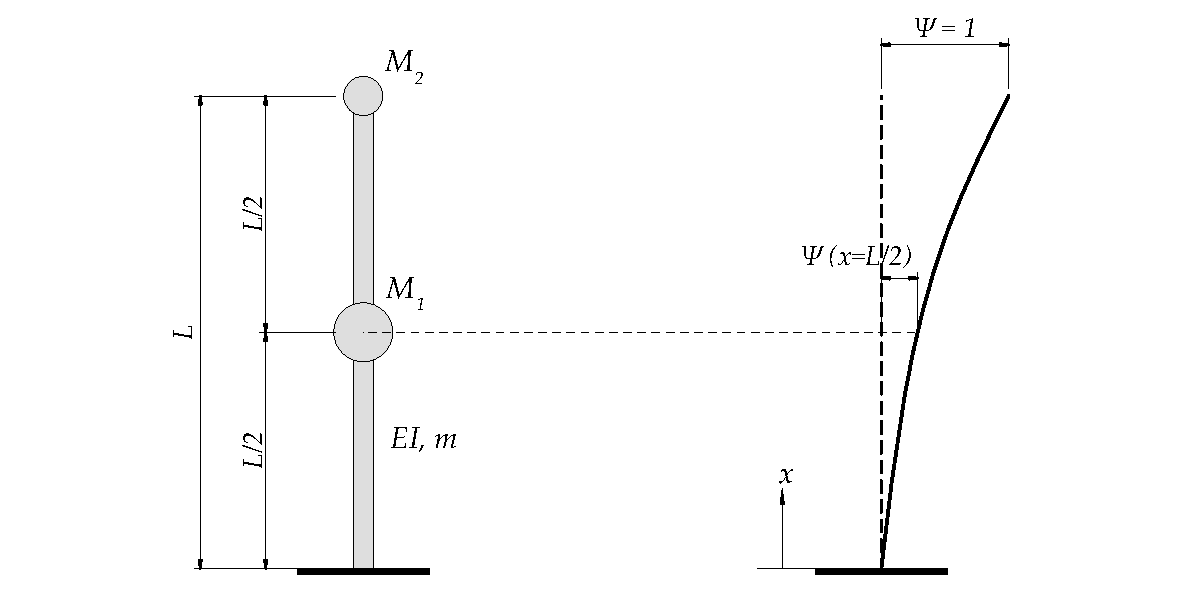
\includegraphics{index_files/mediabag/bilder/aufgabe_rayleigh_2_massen.pdf}

}

\caption{\label{fig-kragarm_2_punkte}Kragarm mit verteilter Masse und
zwei Punktmassen}

\end{figure}

Gesucht:

\begin{itemize}
\tightlist
\item
  Grundfrequenz (1. Eigenfrequenz \(\omega_n\)) des Systems, berechnet
  mit dem Rayleigh-Quotienten.
\end{itemize}

Gegeben:

\begin{itemize}
\tightlist
\item
  Randbedingungen für den Spezialfall:
  \(m_{const} = 0 \text{ und } m_1 = m_2 = m\)
\item
  Formfunktion: \[ \Psi(x) = 1 - \cos(\frac{\pi x}{2L})\]
\end{itemize}

\newpage{}

\hypertarget{sec-ml_2punktmassen}{%
\section{Musterlösung}\label{sec-ml_2punktmassen}}

\hypertarget{grundfrequenz}{%
\subsection{Grundfrequenz}\label{grundfrequenz}}

Mithilfe der in der Vorlesung hergeleiteten Bewegungsgleichung kann
anhand der Formfunktion \(\Psi\) die erste Eigenkreisfrequenz ermittelt
werden. Der Rayleigh-Quotient ist eine Energiebetrachtung. Er setzt die
potentielle, maximale Energie \(E_{pot,max}\) zur kinetischen, maximalen
Energie \(E_{kin,max}\) ins Verhältnis. Daraus lässt sich die
Kreisfrequenz \(\omega_n\) herauslösen.

\begin{equation}\protect\hypertarget{eq-rayleigh_2pm_bewegungsgleichung}{}{
u'' \int_0^L m\Psi^2 dx + u \int_0^L (EI(\Psi'')^2)dx = f(x,t)
}\label{eq-rayleigh_2pm_bewegungsgleichung}\end{equation}

Durch Substitution resultiert die bekannte Bewegungsgleichung:

\begin{equation}\protect\hypertarget{eq-rayleigh_2pm_bewegungsgleichung_allg}{}{
m^\star u'' + k^\star u  = f(x,t) 
\text{ mit } k^\star = \int_0^L (EI(\Psi'')^2)dx 
\text{ und } m^\star = \int_0^L m\Psi^2dx
}\label{eq-rayleigh_2pm_bewegungsgleichung_allg}\end{equation}

Aus der Bewegungsgleichung kann die Eigenkreisfrequenz ermittelt werden:

\begin{equation}\protect\hypertarget{eq-rayleigh_2pm_grundfreq}{}{
\omega_1 = \sqrt{\frac{k^\star}{m^\star}}
}\label{eq-rayleigh_2pm_grundfreq}\end{equation}

\hypertarget{berechnung-der-masse}{%
\subsubsection{Berechnung der Masse}\label{berechnung-der-masse}}

Die Masse in Gleichung~\ref{eq-rayleigh_2pm_grundfreq} kann mittels der
Lösung des Integrals in
Gleichung~\ref{eq-rayleigh_2pm_bewegungsgleichung_allg} bestimmt werden.
Dabei sind die Punktmassen mittels der entsprechenden Deformation an den
Stellen \(L\) und \(\frac{L}{2}\) zu berücksichtigen, sowie die
verteilte Masse über die gesamte Länge.

\begin{equation}m^{\star} = \Psi(x=L)^{2} m_{2} + \Psi(x=L/2)^{2} m_{1} + \int\limits_{0}^{L} \Psi^{2} m\, dx\end{equation}

\begin{equation}\Psi(x)^{2} = \left(1 - \cos{\left(\frac{\pi x}{2 L} \right)}\right)^{2}\end{equation}

\begin{equation}m^{\star} = m \left(- \frac{4 L}{\pi} + \frac{3 L}{2}\right) + m_{1} \left(1 - \frac{\sqrt{2}}{2}\right)^{2} + m_{2}\end{equation}

\hypertarget{berechnung-der-steifigkeit}{%
\subsubsection{Berechnung der
Steifigkeit}\label{berechnung-der-steifigkeit}}

Die Steifigkeit in Gleichung~\ref{eq-rayleigh_2pm_grundfreq} kann
mittels der Lösung des Integrals in
Gleichung~\ref{eq-rayleigh_2pm_bewegungsgleichung_allg} bestimmt werden.
Zur Ermittlung der Steifigkeit \(k^\star\) muss zuerst der Ansatz
zweimal nach \(x\) abgeleitet werden.

\begin{equation}\Psi{\left(x \right)} = 1 - \cos{\left(\frac{\pi x}{2 L} \right)}\end{equation}

\begin{equation}\frac{d}{d x} \Psi{\left(x \right)} = \frac{\pi \sin{\left(\frac{\pi x}{2 L} \right)}}{2 L}\end{equation}

\begin{equation}\frac{d^{2}}{d x^{2}} \Psi{\left(x \right)} = \frac{\pi^{2} \cos{\left(\frac{\pi x}{2 L} \right)}}{4 L^{2}}\end{equation}

Durch das Einsetzen der zweiten Ableitung in den Anteil für \(k^\star\)
aus Gleichung~\ref{eq-rayleigh_2pm_bewegungsgleichung_allg} resultiert
die Steifigkeit zu:

\begin{equation}\protect\hypertarget{eq-rayleigh_2pm_steifigkeit}{}{
k^\star = (\frac{\pi}{2L})^4 \int_0^L(EI(\cos(\frac{\pi x}{2L})^2)) dx
}\label{eq-rayleigh_2pm_steifigkeit}\end{equation}

Durch die Lösung des Integrals folgt:

\begin{equation}k^{\star} = \frac{\pi^{4} E I}{32 L^{3}}\end{equation}

\hypertarget{berechnung-der-grundfrequenz}{%
\subsubsection{Berechnung der
Grundfrequenz}\label{berechnung-der-grundfrequenz}}

Durch das Einsetzen der berechneten Werte resultiert die
Eigenkreisfrequenz in Gleichung~\ref{eq-rayleigh_2pm_grundfreq} zu:

\begin{equation}\omega_{1} = \sqrt{\frac{\pi^{4} E I}{32 L^{3} \left(m \left(- \frac{4 L}{\pi} + \frac{3 L}{2}\right) + m_{1} \left(1 - \frac{\sqrt{2}}{2}\right)^{2} + m_{2}\right)}}\end{equation}

\hypertarget{auswertung-des-spezialfalls}{%
\subsubsection{Auswertung des
Spezialfalls}\label{auswertung-des-spezialfalls}}

Mit Hilfe der Randbedingungen für den Spezialfall aus der
Aufgabenstellung resultiert die Grundfrequenz zu:

\begin{equation}\omega_{1} = \frac{\sqrt{2} \pi^{2} \sqrt{\frac{E I}{M \left(1 - \frac{\sqrt{2}}{2}\right)^{2} + M}}}{8 L^{\frac{3}{2}}}\end{equation}

\begin{equation}\omega_{1} = \frac{1.67 \sqrt{\frac{E I}{M}}}{L^{\frac{3}{2}}}\end{equation}

Die exakte erste Eigenfrequenz eines Zweimassenschwingers mit konstanter
Steifigkeit und gleichen Massen, mit enstsprechenden Randbedingungen
gemäss der Aufgabenstellung, ist:

\begin{equation}\protect\hypertarget{eq-rayleigh_2pm_exakt}{}{
\omega_1 \simeq \sqrt{\frac{3.007\frac{EI}{L^3}}{1.102 M}} = 1.652 \sqrt{\frac{EI}{ML^3}} = \frac{1.652 \sqrt{\frac{E I}{M}}}{L^{\frac{3}{2}}}
}\label{eq-rayleigh_2pm_exakt}\end{equation}

Die Berechnung mit Hilfe des Rayleigh-Quotienten stellt also eine (sehr)
gute Abschätzung der ersten Eigenfrequenz dar.

\hypertarget{beispiel-kargarm-mit-1-punktmasse}{%
\chapter{Beispiel: Kargarm mit 1
Punktmasse}\label{beispiel-kargarm-mit-1-punktmasse}}

\hypertarget{aufgabenstellung-1}{%
\section{Aufgabenstellung}\label{aufgabenstellung-1}}

Das in Abbildung~\ref{fig-kragarm_1_punkte} dargestellte System stellt
einen Kragarm mit verteilter Masse und einer Punktmasse dar. Eine
mögliche Formfunktion ist rechts daneben gezeigt.

\begin{figure}[H]

{\centering 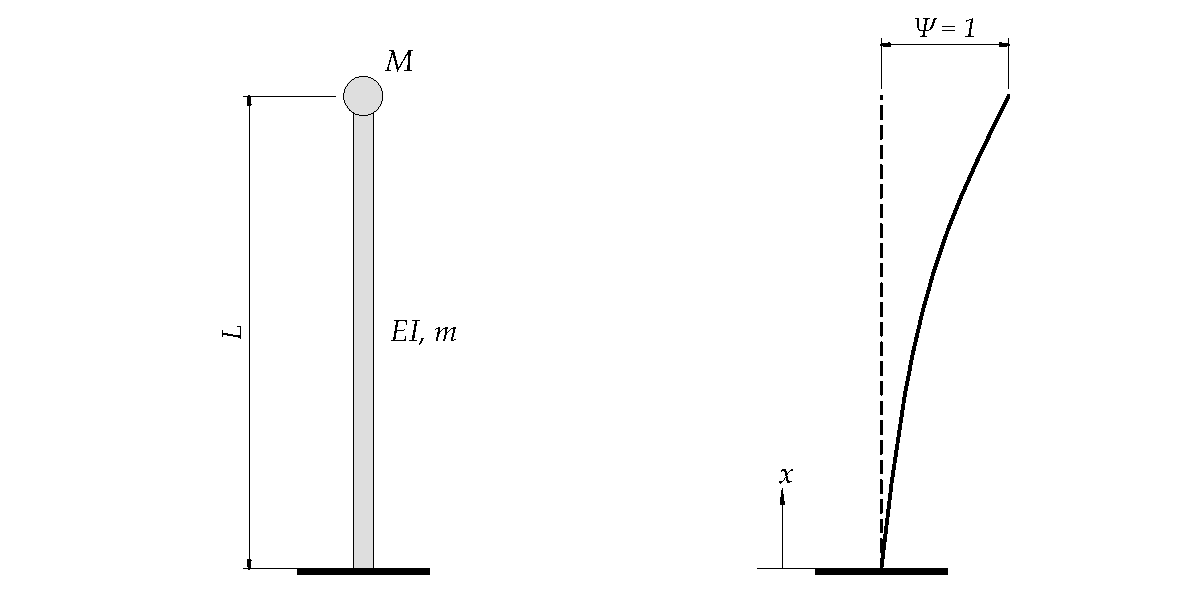
\includegraphics{index_files/mediabag/bilder/aufgabe_rayleigh_1_masse.pdf}

}

\caption{\label{fig-kragarm_1_punkte}Kragarm mit verteilter Masse und
einer Punktmasse}

\end{figure}

Gesucht:

\begin{itemize}
\tightlist
\item
  Grundfrequenz (1. Eigenfrequenz \(\omega_n\)) des Systems in
  Abbildung~\ref{fig-kragarm_1_punkte}, berechnet mit dem
  Rayleigh-Quotienten.
\end{itemize}

Gegeben:

\begin{itemize}
\tightlist
\item
  Ausgewertet für den Spezialfall: \(m_{const} = 0 \text{ und } m = m\)
\item
  Formfunktion: \[ \Psi(x) = 1 - \cos(\frac{\pi x}{2L})\]
\end{itemize}

\newpage{}

\hypertarget{musterluxf6sung}{%
\section{Musterlösung}\label{musterluxf6sung}}

Das Vorgehen entspricht dem Vorgehen in
Kapitel~\ref{sec-ml_2punktmassen}.

\hypertarget{grundfrequenz-1}{%
\subsection{Grundfrequenz}\label{grundfrequenz-1}}

\hypertarget{berechnung-der-masse-1}{%
\subsubsection{Berechnung der Masse}\label{berechnung-der-masse-1}}

Die Masse in Gleichung~\ref{eq-rayleigh_2pm_grundfreq} kann mittels der
Lösung des Integrals in
Gleichung~\ref{eq-rayleigh_2pm_bewegungsgleichung_allg} bestimmt werden.
Dabei ist die Punktmasse mittels der entsprechenden Deformation an der
Stelle \(L\) zu berücksichtigen, sowie die verteilte Masse über die
gesamte Länge.

\begin{equation}m^{\star} = \Psi(x=L)^{2} m + \int\limits_{0}^{L} \Psi^{2} m_{const}\, dx\end{equation}

\begin{equation}\Psi(x)^{2} = \left(1 - \cos{\left(\frac{\pi x}{2 L} \right)}\right)^{2}\end{equation}

\begin{equation}m^{\star} = m + m_{const} \left(- \frac{4 L}{\pi} + \frac{3 L}{2}\right)\end{equation}

\hypertarget{berechnung-der-steifigkeit-1}{%
\subsubsection{Berechnung der
Steifigkeit}\label{berechnung-der-steifigkeit-1}}

Die Steifigkeit in Gleichung~\ref{eq-rayleigh_2pm_grundfreq} kann
mittels der Lösung des Integrals in
Gleichung~\ref{eq-rayleigh_2pm_bewegungsgleichung_allg} bestimmt werden.
Zur Ermittlung der Steifigkeit \(k^\star\) muss zuerst der Ansatz
zweimal nach \(x\) abgeleitet werden.

\begin{equation}\Psi{\left(x \right)} = 1 - \cos{\left(\frac{\pi x}{2 L} \right)}\end{equation}

\begin{equation}\frac{d}{d x} \Psi{\left(x \right)} = \frac{\pi \sin{\left(\frac{\pi x}{2 L} \right)}}{2 L}\end{equation}

\begin{equation}\frac{d^{2}}{d x^{2}} \Psi{\left(x \right)} = \frac{\pi^{2} \cos{\left(\frac{\pi x}{2 L} \right)}}{4 L^{2}}\end{equation}

Durch das Einsetzen der zweiten Ableitung in den Anteil für \(k^\star\)
aus Gleichung~\ref{eq-rayleigh_2pm_bewegungsgleichung_allg} resultiert
die Steifigkeit zu:

\begin{equation}\protect\hypertarget{eq-rayleigh_1pm_steifigkeit}{}{
k^\star = (\frac{\pi}{2L})^4 \int_0^L(EI(\cos(\frac{\pi x}{2L})^2)) dx
}\label{eq-rayleigh_1pm_steifigkeit}\end{equation}

Durch die Lösung des Integrals folgt:

\begin{equation}k^{\star} = \frac{\pi^{4} E I}{32 L^{3}}\end{equation}

\hypertarget{berechnung-der-grundfrequenz-1}{%
\subsubsection{Berechnung der
Grundfrequenz}\label{berechnung-der-grundfrequenz-1}}

Durch das Einsetzen der berechneten Werte resultiert die
Eigenkreisfrequenz in Gleichung~\ref{eq-rayleigh_2pm_grundfreq} zu:

\begin{equation}\omega_{1} = \sqrt{\frac{\pi^{4} E I}{32 L^{3} \left(m + m_{const} \left(- \frac{4 L}{\pi} + \frac{3 L}{2}\right)\right)}}\end{equation}

\hypertarget{auswertung-des-spezialfalls-1}{%
\subsubsection{Auswertung des
Spezialfalls}\label{auswertung-des-spezialfalls-1}}

Mit Hilfe der Randbedingungen für den Spezialfall aus der
Aufgabenstellung resultiert die Grundfrequenz zu:

\begin{equation}\omega_{1} = \frac{\sqrt{2} \pi^{2} \sqrt{\frac{E I}{m}}}{8 L^{\frac{3}{2}}}\end{equation}

\begin{equation}\omega_{1} = \frac{1.74 \sqrt{\frac{E I}{m}}}{L^{\frac{3}{2}}}\end{equation}

\hypertarget{beispiel-einfacher-balken-mit-konstanter-masse}{%
\chapter{Beispiel: Einfacher Balken mit konstanter
Masse}\label{beispiel-einfacher-balken-mit-konstanter-masse}}

\hypertarget{aufgabenstellung-2}{%
\section{Aufgabenstellung}\label{aufgabenstellung-2}}

Das System in Abbildung~\ref{fig-rayleigh_balken_system} zeigt einen
einfachen Balken mit einer konstanten Streckenlast belastet.

\begin{figure}[H]

{\centering 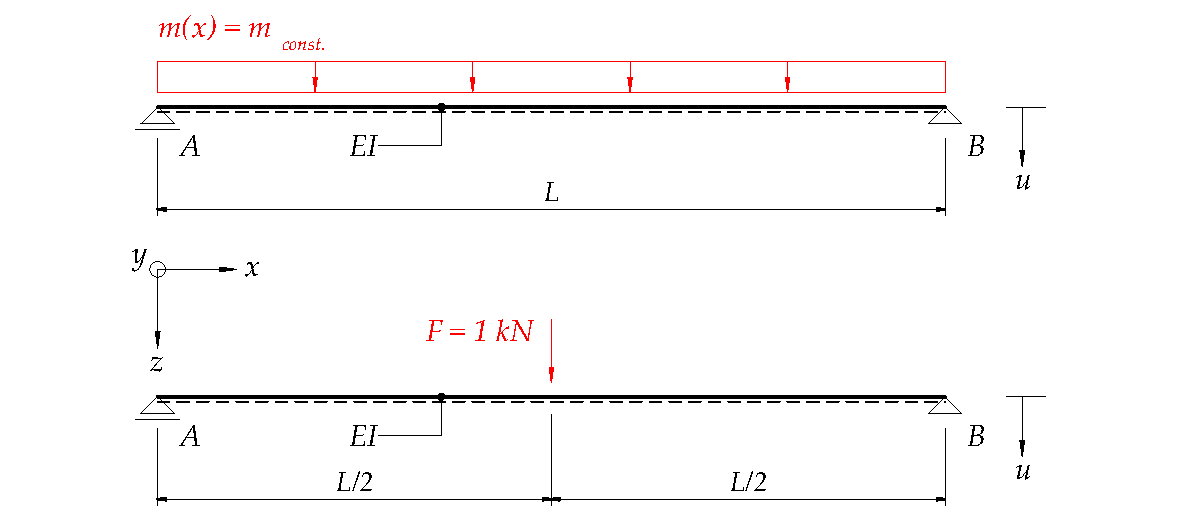
\includegraphics{index_files/mediabag/bilder/aufgabe_rayleigh_balken.pdf}

}

\caption{\label{fig-rayleigh_balken_system}Statisches System des
einfachen Balkens}

\end{figure}

Gesucht:

\begin{itemize}
\tightlist
\item
  Eigenkreisfrequenz \(\omega_1\) mit Hilfe der analytischen
  Formfunktion
  Gleichung~\ref{eq-rayleigh_balken_analytisch_formfunktion}
  \begin{equation}\protect\hypertarget{eq-rayleigh_balken_analytisch_formfunktion}{}{
  \Psi(x) = \sin{\frac{\pi x}{L}}
  }\label{eq-rayleigh_balken_analytisch_formfunktion}\end{equation}
\item
  Eigenkreisfrequenz \(\omega_1\) mit Hilfe der Biegelinie
\end{itemize}

Gegeben:

\begin{itemize}
\tightlist
\item
  Länge des Balkens \(L\)
\item
  Verteilte Masse ist konstant \(m_{const}\)
\item
  Exakte Lösung der Eigenkreisfrequenz gemäss
  Gleichung~\ref{eq-rayleigh_balken_exakt}
\end{itemize}

\begin{equation}\protect\hypertarget{eq-rayleigh_balken_exakt}{}{
\omega_1 = \pi^2 \cdot \sqrt{\frac{E\cdot I}{m_{const}\cdot L^4}}
}\label{eq-rayleigh_balken_exakt}\end{equation}

\newpage{}

\hypertarget{musterluxf6sung-1}{%
\section{Musterlösung}\label{musterluxf6sung-1}}

\hypertarget{analytische-formfunktion}{%
\subsection{Analytische Formfunktion}\label{analytische-formfunktion}}

Als Formfunktion wird eine Sinus-Funktion gewählt. Dabei ist
sicherzustellen, dass die Formfunktion normiert ist. Das heisst, der
maximale Wert der Funktion ist \(1\). Dazu sind die kinematischen
Randbedingungen einzuhalten. Entsprechend des Systems in
Abbildung~\ref{fig-rayleigh_balken_system} muss die Verformung bei den
Lagern null sein. Die gewählte Formfunktion bedingt keine weitere
Anpassung zur Normierung.

\begin{equation}\Psi{\left(x \right)} = \sin{\left(\frac{\pi x}{L} \right)}\end{equation}

\begin{figure}[H]

{\centering 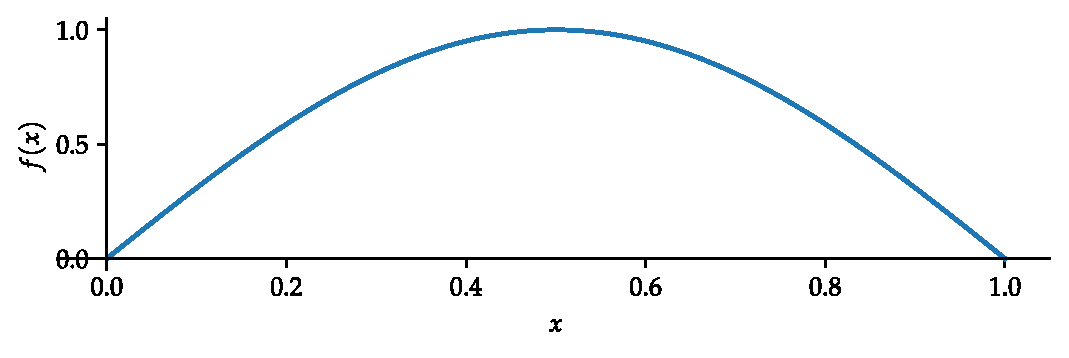
\includegraphics{index_files/mediabag/rayleigh_03_files/figure-pdf/fig-formfunktion-output-1.pdf}

}

\caption{\label{fig-formfunktion}Frei gewählte Formfunktion}

\end{figure}

\hypertarget{rayleigh---quotient-1}{%
\subsubsection{Rayleigh - Quotient}\label{rayleigh---quotient-1}}

Der Rayleigh-Quotient ist eine Energiebetrachtung. Er setzt die
potentielle, maximale Energie \(E_{pot,max}\) zur kinetischen, maximalen
Energie \(E_{kin,max}\) ins Verhältnis. Daraus lässt sich die
Kreisfrequenz \(\omega_n\) herauslösen. Die Lösung der Integrale wird
hier mit einer Mathematik-Software durchgeführt. Die einzelnen
Teilschritte werden nicht aufgeführt.
\begin{equation}\protect\hypertarget{eq-rayleigh_balken_energie}{}{
E_{pot,max} = E_{kin,max}
}\label{eq-rayleigh_balken_energie}\end{equation}

\begin{equation}\protect\hypertarget{eq-rayleigh_balken_quotient}{}{
\omega_1^2 = \frac{\int_0^L EI[u''(x)]^2 dx}{\int_0^L m_{const.}[u(x)]^2 dx}
}\label{eq-rayleigh_balken_quotient}\end{equation}

Dies lässt sich mit entsprechender Formfunktion schreiben:

\begin{equation}\protect\hypertarget{eq-rayleigh_balken_quotient_subs}{}{
\omega_1^2 = \frac{\int_0^L EI[\Psi''(x)]^2 dx}{\int_0^L m_{const.}[\Psi(x)]^2 dx}
}\label{eq-rayleigh_balken_quotient_subs}\end{equation}

Durch die Ermittlung der zweiten Ableitung der Formfunktion:

\begin{equation}\Psi{\left(x \right)} = \sin{\left(\frac{\pi x}{L} \right)}\end{equation}

\begin{equation}\frac{d}{d x} \Psi{\left(x \right)} = \frac{\pi \cos{\left(\frac{\pi x}{L} \right)}}{L}\end{equation}

\begin{equation}\frac{d^{2}}{d x^{2}} \Psi{\left(x \right)} = - \frac{\pi^{2} \sin{\left(\frac{\pi x}{L} \right)}}{L^{2}}\end{equation}

Diese eingesetzt in die
Gleichung~\ref{eq-rayleigh_balken_quotient_subs}:

\begin{equation}\omega_{1} = \frac{\pi^{2} \sqrt{\frac{E I}{m_{const}}}}{L^{2}}\end{equation}

Dies entspricht der exakten Lösung
Gleichung~\ref{eq-rayleigh_balken_exakt}! Grund dafür ist, dass die
gewählte Formfunktion mit der dynamischen Deformation übereinstimmt.

\hypertarget{formfunktion-aus-biegelinie}{%
\subsection{Formfunktion aus
Biegelinie}\label{formfunktion-aus-biegelinie}}

Die Biegelinie für das System in
Abbildung~\ref{fig-rayleigh_balken_system} ist folgend beschrieben.
Beachte dabei dass die Deformation nach \emph{``unten''} positiv
definiert ist. Die Funktion kann aus Hilfswerken entnommen werden.

\begin{equation}w{\left(x \right)} = \begin{cases} \frac{F L^{2} x \left(\frac{3}{4} - \frac{x^{2}}{L^{2}}\right)}{12 E I} & \text{for}\: x \leq \frac{L}{2} \\\frac{F \left(x \left(3 L^{2} - 4 x^{2}\right) - \left(L - 2 x\right)^{3}\right)}{48 E I} & \text{otherwise} \end{cases}\end{equation}

\begin{figure}[H]

{\centering 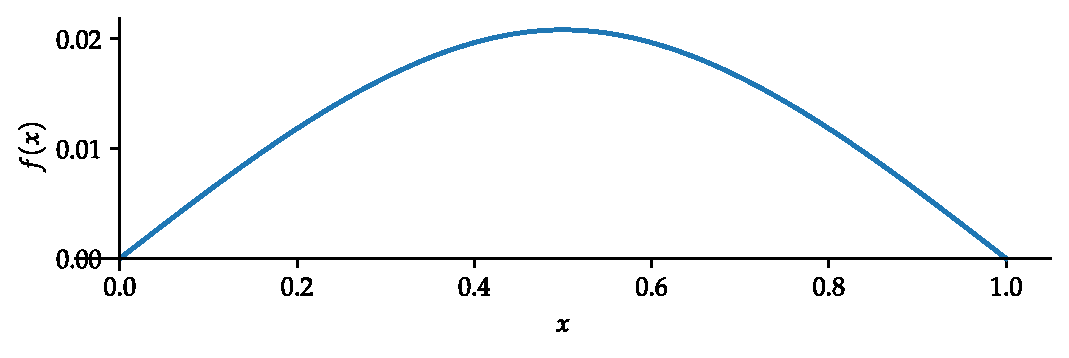
\includegraphics{index_files/mediabag/rayleigh_03_files/figure-pdf/fig-formfunktion_biege-output-1.pdf}

}

\caption{\label{fig-formfunktion_biege}Formfunktion aus Biegelinie
abgeleitet}

\end{figure}

\hypertarget{normierung}{%
\subsubsection{Normierung}\label{normierung}}

Es ist ersichtlich, dass die Formfunktion noch eine Normierung benötigt.
Dazu wird der Maximalwert zu \(1\) gesetzt. Die Randbedingungen sind
bereits erfüllt.

\begin{equation}w_{norm}{\left(x \right)} = \frac{48 E I \left(\begin{cases} \frac{F L^{2} x \left(\frac{3}{4} - \frac{x^{2}}{L^{2}}\right)}{12 E I} & \text{for}\: x \leq \frac{L}{2} \\\frac{F \left(x \left(3 L^{2} - 4 x^{2}\right) - \left(L - 2 x\right)^{3}\right)}{48 E I} & \text{otherwise} \end{cases}\right)}{F L^{3}}\end{equation}

\begin{figure}[H]

{\centering 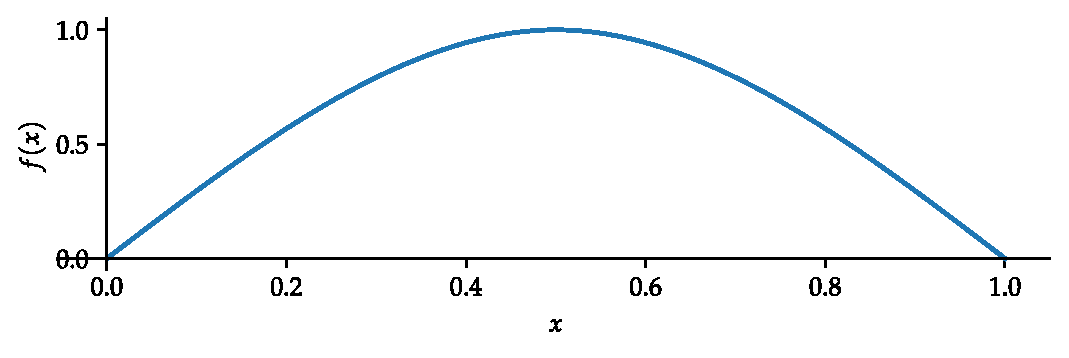
\includegraphics{index_files/mediabag/rayleigh_03_files/figure-pdf/fig-formfunktion_biege_norm-output-1.pdf}

}

\caption{\label{fig-formfunktion_biege_norm}Normierte Formfunktion aus
Biegelinie abgeleitet}

\end{figure}

\hypertarget{rayleigh---quotient-2}{%
\subsubsection{Rayleigh - Quotient}\label{rayleigh---quotient-2}}

Durch das Einsetzen der bestimmten Formfunktion aus der Biegelinie in
Gleichung~\ref{eq-rayleigh_balken_quotient_subs} kann die
Eigenkreisfrequenz ermittelt werden.

\begin{equation}\omega_{1 biege} = \frac{9.94 \left(\frac{E I}{m_{const}}\right)^{0.5}}{L^{2}}\end{equation}

\hypertarget{vergleich-beider-luxf6sungen}{%
\subsection{Vergleich beider
Lösungen}\label{vergleich-beider-luxf6sungen}}

Ein Vergleich der Eigenkreisfrequenz aus der Biegeform mit der exakten
Lösung aus Gleichung~\ref{eq-rayleigh_balken_exakt} zeigt eine minimale
Abweichung.

\begin{equation}\text{Abweichung} = 0.72 \%\end{equation}

\begin{figure}[H]

{\centering 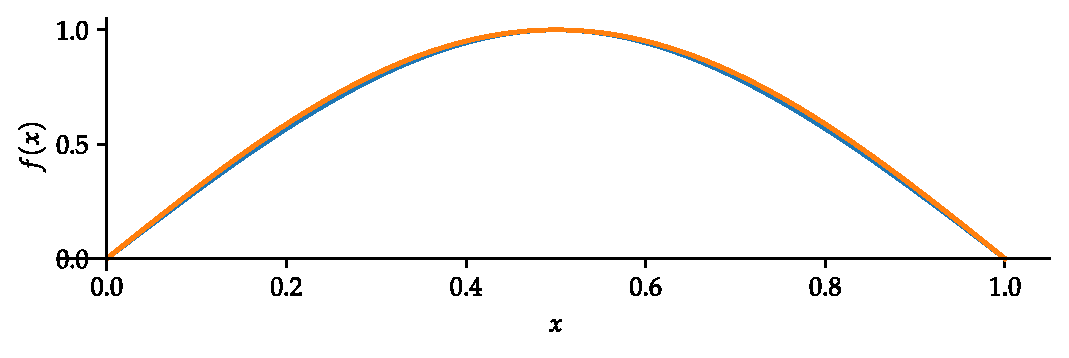
\includegraphics{index_files/mediabag/rayleigh_03_files/figure-pdf/fig-formfunktion_vergleich-output-1.pdf}

}

\caption{\label{fig-formfunktion_vergleich}Überlagerung beider
Funktionen}

\end{figure}

Um die minimale Abweichung offensichtlicher darzustellen ist in
Abbildung~\ref{fig-ausschnitt_formfunktion_vergleich} ein Teilbereich
dargestellt.

\begin{figure}[H]

{\centering 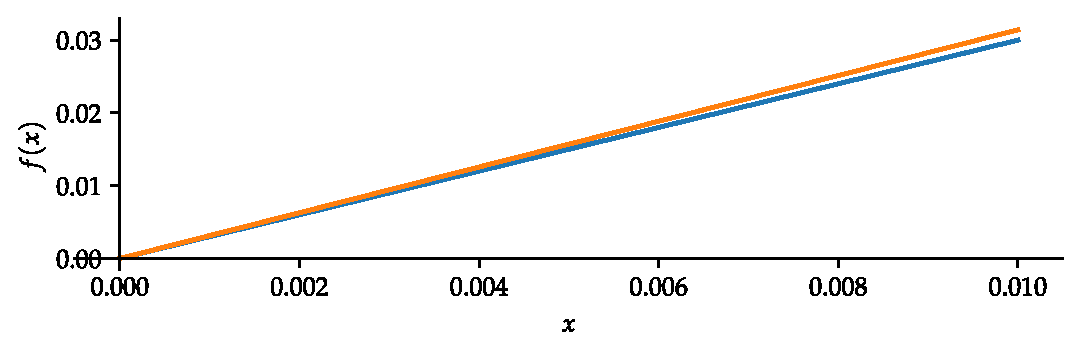
\includegraphics{index_files/mediabag/rayleigh_03_files/figure-pdf/fig-ausschnitt_formfunktion_vergleich-output-1.pdf}

}

\caption{\label{fig-ausschnitt_formfunktion_vergleich}Ausschnitt der
Überlagerung beider Funktionen}

\end{figure}

\part{Einmassenschwinger}

\hypertarget{beispiel-logarithmisches-dekrement}{%
\chapter{Beispiel: Logarithmisches
Dekrement}\label{beispiel-logarithmisches-dekrement}}

\hypertarget{aufgabenstellung-3}{%
\section{Aufgabenstellung}\label{aufgabenstellung-3}}

Das in Abbildung~\ref{fig-ems_log_dek_system} dargestellte System zeigt
ein Rahmentragwerk. Dieses kann als Einmassenschwinger modelliert
werden, welcher eine gedämpfte freie Schwingung erfährt.

\begin{figure}[H]

{\centering 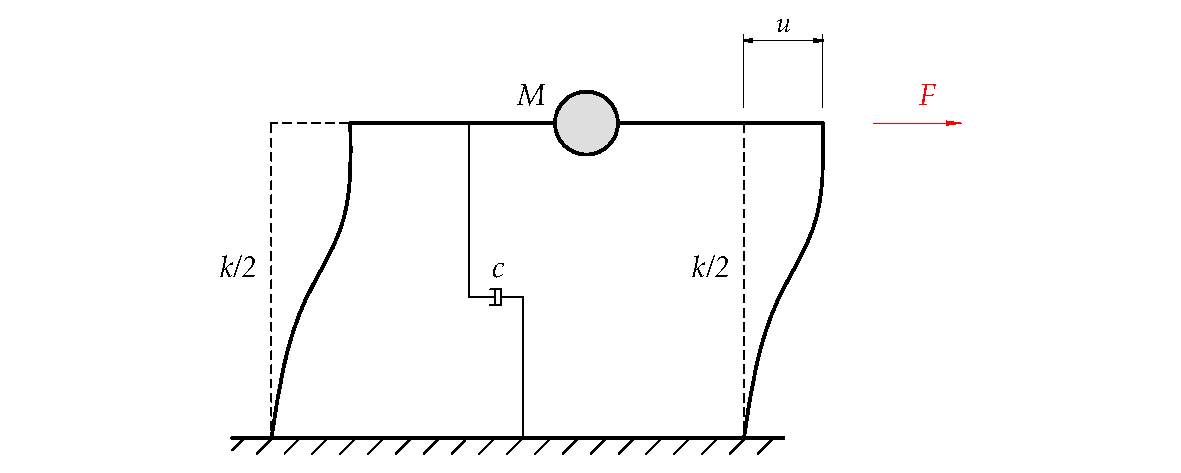
\includegraphics{index_files/mediabag/bilder/aufgabe_ems_log_dek.pdf}

}

\caption{\label{fig-ems_log_dek_system}Am Riegel ausgelenktes System}

\end{figure}

Um die Systemeigenschaften des Rahmens zu untersuchen, wird eine
Kopfverschiebung bzw. Auslenkung des Rahmens von \(u_0 = 20\text{ mm}\)
aufgebracht. Danach wird die Halterung schlagartig gelöst und der Rahmen
kann frei schwingen. Die angebrachte Messeinrichtung registriert eine
max. Kopfverschiebung nach dem ersten Zurückschwingen von
\(u_1 = 15\text{ mm}\) nach \(T_D = 0.2 \text{s}\).

Gesucht:

\begin{itemize}
\tightlist
\item
  Laterale bzw. horizontale Steifigkeit \(k\) des Rahmens
\item
  Die Dämpfungsrate \(\zeta\) und die Dämpfungskonstante \(c\)
\item
  Die Amplitude der Auslenkung des Rahmens nach 10 Schwingzyklen
\end{itemize}

Gegeben:

\hypertarget{tbl-parameter_log_dekrement}{}
\begin{longtable}[]{@{}
  >{\raggedright\arraybackslash}p{(\columnwidth - 2\tabcolsep) * \real{0.5000}}
  >{\raggedright\arraybackslash}p{(\columnwidth - 2\tabcolsep) * \real{0.5000}}@{}}
\caption{\label{tbl-parameter_log_dekrement}Parameter der
Aufgabenstellung}\tabularnewline
\toprule\noalign{}
\endfirsthead
\endhead
\bottomrule\noalign{}
\endlastfoot
\(EA_{riegel} = \infty\) & \(EA_{stuetze} = \infty\) \\
\(EI_{riegel} = \infty\) & \(T_{D} = 0.2 \text{s}\) \\
\(m = \frac{1941 \text{N} \text{s}^{2}}{\text{m}}\) &
\(u_{0} = 20 \text{mm}\) \\
\(u_{1} = 15 \text{mm}\) & \\
\end{longtable}

\newpage{}

\hypertarget{sec-ml_log_dek}{%
\section{Musterlösung}\label{sec-ml_log_dek}}

\hypertarget{horizontale-steifigkeit}{%
\subsection{Horizontale Steifigkeit}\label{horizontale-steifigkeit}}

\hypertarget{logarithmisches-dekrement}{%
\subsubsection{Logarithmisches
Dekrement}\label{logarithmisches-dekrement}}

Da keine Angaben über die Profile der Stützen gemacht werden, kann
mittels des logarithmischen Dekrements die Eigenkreisfrequenz bestimmt
werden. Anhand der Eigenkreisfrequenz lässt sich die Steifigkeit
ableiten.

\begin{figure}[H]

{\centering 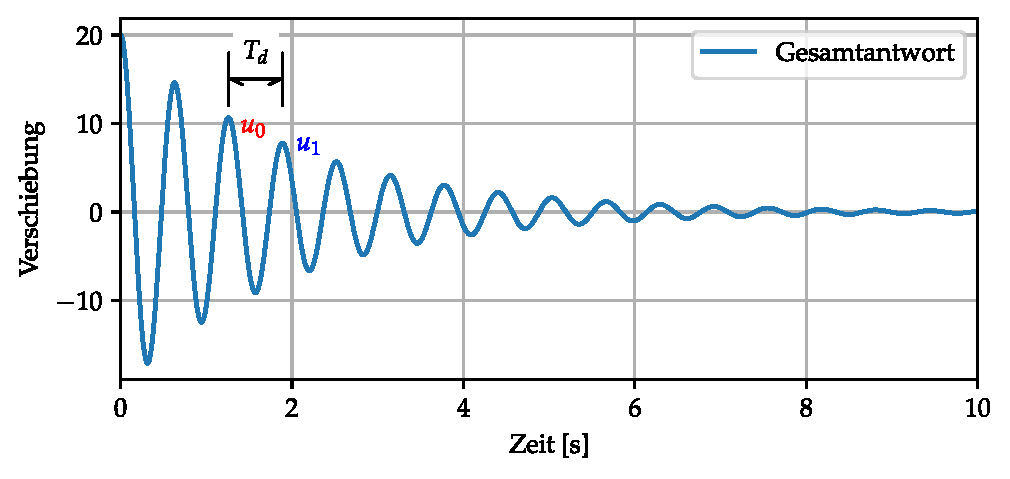
\includegraphics{index_files/mediabag/ems_01_files/figure-pdf/fig-ems_log_dek_zerfall-output-1.pdf}

}

\caption{\label{fig-ems_log_dek_zerfall}Beispiel eines logarithmischen
Dekrements}

\end{figure}

\begin{equation}\delta = \log{\left(\frac{u_{0}}{u_{1}} \right)}\end{equation}

\begin{equation}\delta = 0.288\end{equation}

\hypertarget{duxe4mpfungsrate}{%
\subsubsection{Dämpfungsrate}\label{duxe4mpfungsrate}}

Anhand des logarithmischen Dekrements kann die Dämpfungsrate bestimmt
werden.

\begin{figure}[H]

{\centering 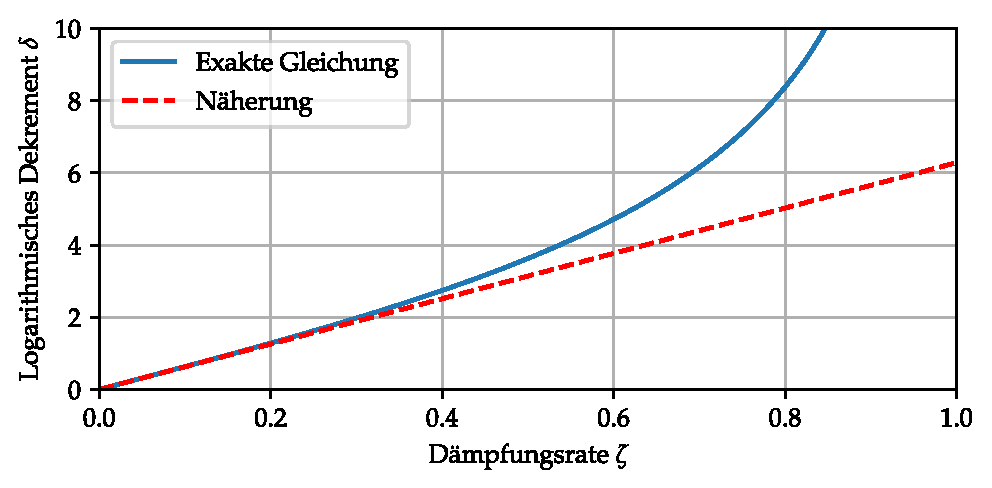
\includegraphics{index_files/mediabag/ems_01_files/figure-pdf/fig-ems_log_dek_daempfungsrate-output-1.pdf}

}

\caption{\label{fig-ems_log_dek_daempfungsrate}Dämpfungsrate anhand des
logarithmischen Dekrements}

\end{figure}

Für kleine Dämpfungsraten kann folgende Gleichung verwendet werden:

\begin{equation}\protect\hypertarget{eq-ems_log_dek_daempfungsrate_approx}{}{
\zeta \simeq \frac{\delta}{2\pi}
}\label{eq-ems_log_dek_daempfungsrate_approx}\end{equation}

Die exakte Lösung bestimmt sich folgender massen:

\begin{equation}\zeta_{} = \frac{\delta}{\sqrt{\delta^{2} + 4 \pi^{2}}}\end{equation}

\begin{equation}\zeta_{} = \frac{\log{\left(\frac{u_{0}}{u_{1}} \right)}}{\sqrt{\log{\left(\frac{u_{0}}{u_{1}} \right)}^{2} + 4 \pi^{2}}}\end{equation}

\begin{equation}\zeta_{} = 0.0457\end{equation}

\hypertarget{eigenkreisfrequenz}{%
\subsubsection{Eigenkreisfrequenz}\label{eigenkreisfrequenz}}

Aus der Aufgabenstellung ist die gedämpfte Periode von \(T_D = 0.2 s\)
bekannt. Anhand dieser lässt sich die \emph{gedämpfte
Eigenkreisfrequenz} \(\omega_D\) bestimmen und unter Berücksichtigung
der Dämpfungsrate \(\zeta\) kann die \emph{Eigenkreisfrequenz}
\(\omega_n\) bestimmt werden.

\begin{equation}\omega_{D} = \frac{2 \pi}{T_{D}}\end{equation}

\begin{equation}\omega_{D} = \frac{31.42}{\text{s}}\end{equation}

\begin{equation}\omega_{n} = \frac{\omega_{D}}{\sqrt{1 - \zeta_{}^{2}}}\end{equation}

\begin{equation}\omega_{n} = \frac{31.45}{\text{s}}\end{equation}

\hypertarget{steifigkeit}{%
\subsubsection{Steifigkeit}\label{steifigkeit}}

Wir kennen die Beziehung zwischen Eigenkreisfrequenz und Steifigkeit:

\begin{equation}\protect\hypertarget{eq-ems_log_dek_kreisfrequenz}{}{
\omega_n = \sqrt{\frac{k}{m}}
}\label{eq-ems_log_dek_kreisfrequenz}\end{equation}

\begin{equation}k = m \omega_{n}^{2}\end{equation}

\begin{equation}k = \frac{1.92 \cdot 10^{6} \text{N}}{\text{m}}\end{equation}

\hypertarget{duxe4mpfungskonstante}{%
\subsection{Dämpfungskonstante}\label{duxe4mpfungskonstante}}

Anhand der Dämpfungsrate \(\zeta\) lässt sich leicht die
Dämpfungskonstante bestimmen:

\begin{equation}\protect\hypertarget{eq-ems_log_dek_daempfungsrate}{}{
\zeta = \frac{c}{2\omega_nm}
}\label{eq-ems_log_dek_daempfungsrate}\end{equation}

\begin{equation}c = \frac{5.58 \cdot 10^{3} \text{N} \text{s}}{\text{m}}\end{equation}

\hypertarget{amplitude-nach-10-schwingzyklen}{%
\subsection{Amplitude nach 10
Schwingzyklen}\label{amplitude-nach-10-schwingzyklen}}

Das Verhalten der Amplitude ist in
Abbildung~\ref{fig-ems_log_dek_zerfall} dargestellt.

\begin{equation}\protect\hypertarget{eq-ems_log_dek_dekrement_10}{}{
\delta = \ln({\frac{u_0}{u_1}})
}\label{eq-ems_log_dek_dekrement_10}\end{equation}

\(\delta\) ist ein konstanter Wert und kann auf 10 Zyklen erweitert
werden.

\begin{equation}u_{1} = u_{0} e^{- \delta}\end{equation}

\begin{equation}u_{10} = u_{0} e^{- 10 \delta}\end{equation}

\begin{equation}u_{10} = 1.126 \text{mm}\end{equation}

\hypertarget{beispiel-impulssatz}{%
\chapter{Beispiel: Impulssatz}\label{beispiel-impulssatz}}

\hypertarget{aufgabenstellung-4}{%
\section{Aufgabenstellung}\label{aufgabenstellung-4}}

Abbildung~\ref{fig-ems_impuls_system} zeigt das System eines
Stahlrahmens. Dieser wird durch eine kurzzeitig einwirkende
Stossbelastung \(F(t)\) in Höhe des Rahmenriegels beansprucht.

\begin{figure}[H]

{\centering 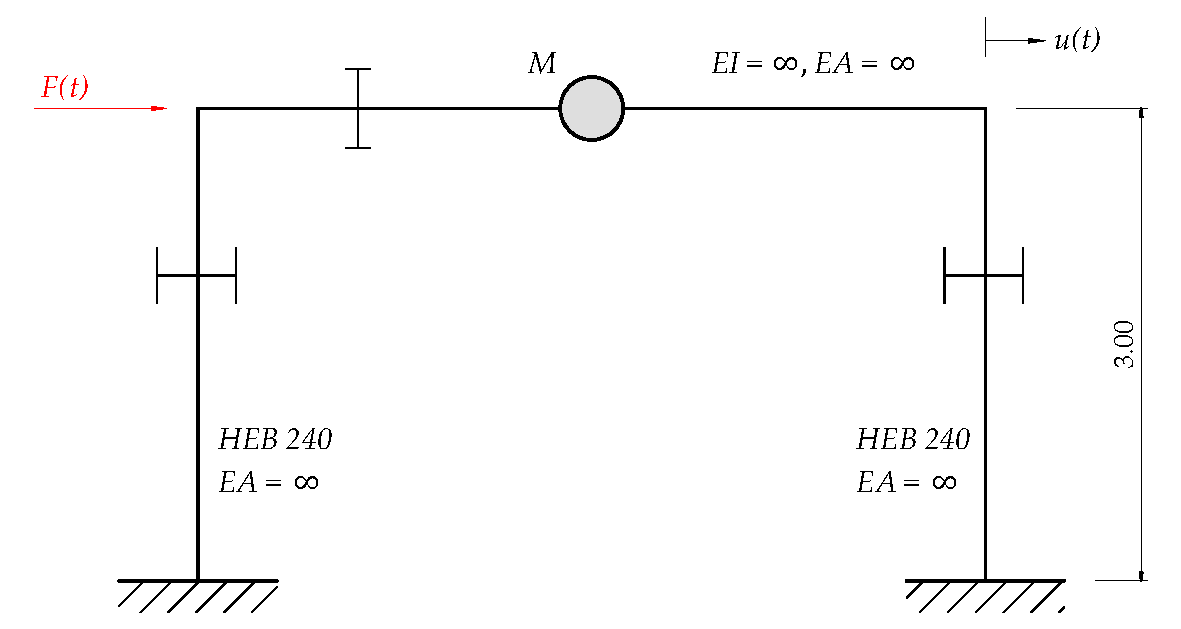
\includegraphics{index_files/mediabag/bilder/aufgabe_ems_impuls.pdf}

}

\caption{\label{fig-ems_impuls_system}System des Stahlramens mit
kurzzeitig einwirkender Stossbelastung}

\end{figure}

Gesucht:

\begin{itemize}
\tightlist
\item
  Der Maximalwert der zu erwartenden Riegelauslenkung (näherungsweise)
\item
  Darstellung des zeitlichen Verlaufs \(u(t)\) in einem Diagramm
\item
  Nachweis der Elastizität des Systems anhand der Rückstellkraft
  (Spannungsnachweis mit Fliessspannung \(f_y\) als Grenze)
\end{itemize}

Gegeben:

\begin{itemize}
\tightlist
\item
  Lastfunktion gemäss Abbildung~\ref{fig-ems_impuls_lastfunktion}
\end{itemize}

\hypertarget{tbl-parameter_impuls}{}
\begin{longtable}[]{@{}
  >{\raggedright\arraybackslash}p{(\columnwidth - 2\tabcolsep) * \real{0.5000}}
  >{\raggedright\arraybackslash}p{(\columnwidth - 2\tabcolsep) * \real{0.5000}}@{}}
\caption{\label{tbl-parameter_impuls}Parameter der
Aufgabenstellung}\tabularnewline
\toprule\noalign{}
\endfirsthead
\endhead
\bottomrule\noalign{}
\endlastfoot
\(EA_{riegel} = \infty\) & \(EA_{stuetze} = \infty\) \\
\(EI_{riegel} = \infty\) &
\(EI_{stuetze} = 23646000.0 \text{m}^{2} \text{N}\) \\
\(F_{max} = 1000000.0 \text{N}\) & \(H = 3000.0 \text{mm}\) \\
\(W_{el y} = 938000.0 \text{mm}^{3}\) &
\(f_{y} = \frac{355.0 \text{N}}{\text{mm}^{2}}\) \\
\(m_{tot} = \frac{5000.0 \text{N} \text{s}^{2}}{\text{m}}\) &
\(t_{1} = 0.003 \text{s}\) \\
\(t_{2} = 0.006 \text{s}\) & \(u_{0} = 0.0\) \\
\end{longtable}

\begin{figure}[H]

{\centering 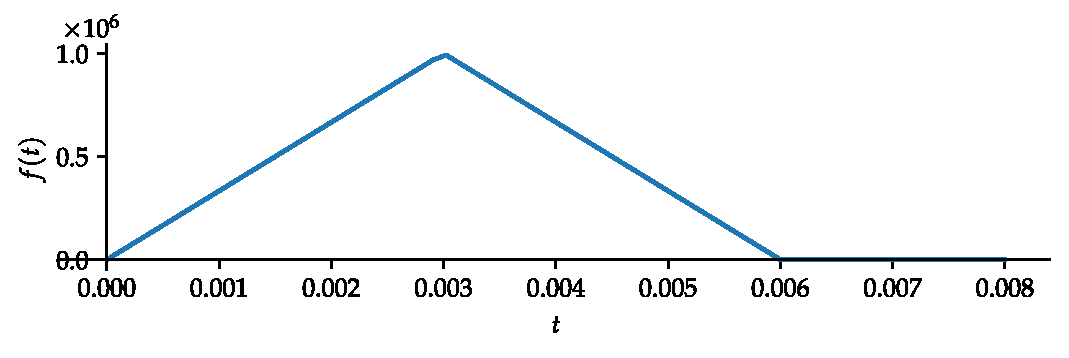
\includegraphics{index_files/mediabag/ems_02_files/figure-pdf/fig-ems_impuls_lastfunktion-output-1.pdf}

}

\caption{\label{fig-ems_impuls_lastfunktion}Lastfunktion der kurzzeitig
einwirkenden Stossbelastung}

\end{figure}

\newpage{}

\hypertarget{musterluxf6sung-2}{%
\section{Musterlösung}\label{musterluxf6sung-2}}

\hypertarget{horizontale-steifigkeit-1}{%
\subsection{Horizontale Steifigkeit}\label{horizontale-steifigkeit-1}}

Für entsprechende Anwendungsfälle gibt es fertige Lösungen zur
Bestimmung der Steifigkeit. Gemäss Abbildung~\ref{fig-ems_impuls_system}
ist die Stütze am Fuss- und Kopfpunkt eingespannt (Änderungen der
Lagerung beeinflussen die Steifigkeit!). Somit resultiert die
Steifigkeit zu:

\begin{equation}\protect\hypertarget{eq-ems_impuls_k_fur_stuetze}{}{
k_{Stuetze} = \frac{12EI_{Stuetze}}{H^3}
}\label{eq-ems_impuls_k_fur_stuetze}\end{equation}

Diese gilt für eine einzelne Stütze. Angewendet auf das Beispiel folgt
die Systemsteifigkeit zu:

\begin{equation}k_{} = \frac{24 EI_{stuetze}}{H^{3}}\end{equation}

\begin{equation}k_{} = \frac{2.1 \cdot 10^{7} \text{N}}{\text{m}}\end{equation}

\hypertarget{eigenkreisfrequenz-1}{%
\subsection{Eigenkreisfrequenz}\label{eigenkreisfrequenz-1}}

\begin{equation}\omega_{n} = \sqrt{\frac{k}{m}}\end{equation}

\begin{equation}\omega_{n} = 2 \sqrt{6} \sqrt{\frac{EI_{stuetze}}{H^{3} m_{tot}}}\end{equation}

\begin{equation}\omega_{n} = \frac{64.8}{\text{s}}\end{equation}

\hypertarget{bewegungsgleichung}{%
\subsection{Bewegungsgleichung}\label{bewegungsgleichung}}

Die Bewegungsgleichung für einen ungedämpften Einmassenschwinger ist die
folgende:

\begin{equation}\protect\hypertarget{eq-ems_impuls_bewegungsgleichung}{}{
m u(t)'' + k u(t) = F(t)
}\label{eq-ems_impuls_bewegungsgleichung}\end{equation}

\hypertarget{approximation-der-luxf6sung}{%
\subsubsection{Approximation der
Lösung}\label{approximation-der-luxf6sung}}

Es handelt sich um eine inhomogene Differentialgleichung 2.Ordnung. Auf
die exakte Lösung der Gleichung wird nicht eingegangen. Es wird versucht
die bemessungsrelevanten Parameter näherungsweise zu bestimmen. Dies
lässt sich mit dem Impulssatz approximieren.

\begin{equation}\protect\hypertarget{eq-ems_impuls_impulssatz}{}{
F \Delta t = m \Delta v
}\label{eq-ems_impuls_impulssatz}\end{equation}

Dieser besagt, dass die einwirkende Kraft \(F\) im betrachteten
Zeitabschnitt \(\Delta t\) der Masse \(m\) multipliziert mit der
Geschwindigkeitsänderung \(\Delta v\) des Objekts entspricht. Für eine
kurze Anregung, wie im Beispiel der Fall ist, kann die
Anfangsgeschwindigkeit wie folgt bestimmt werden:

\begin{equation}\protect\hypertarget{eq-ems_impuls_v0}{}{
v_0 = \frac{I}{m}
}\label{eq-ems_impuls_v0}\end{equation}

\begin{equation}\protect\hypertarget{eq-ems_impuls_intensitaet}{}{
I = \int_{0}^{t_2} F(t) \,dt
}\label{eq-ems_impuls_intensitaet}\end{equation}

\begin{equation}I_{} = 3000.0 \text{N} \text{s}\end{equation}

\begin{equation}v_{0} = \frac{3000.0 \text{N} \text{s}}{m_{tot}}\end{equation}

\begin{equation}v_{0} = \frac{0.6 \text{m}}{\text{s}}\end{equation}

Durch die Impuls-Betrachtung vereinfacht sich die Bewegungsgleichung zu:

\begin{equation}\protect\hypertarget{eq-ems_impuls_bewegungsgleichung_homogen_ungedaempft}{}{
m u(t)'' + k u(t) = 0
}\label{eq-ems_impuls_bewegungsgleichung_homogen_ungedaempft}\end{equation}

Mit der Anfangsgeschwindigkeit als Randbedingung.

\begin{equation}\protect\hypertarget{eq-ems_impuls_r1}{}{
u'(t=0) = v_0  
}\label{eq-ems_impuls_r1}\end{equation}

und der Startauslenkung:

\begin{equation}\protect\hypertarget{eq-ems_impuls_r2}{}{
u(t=0) = u_0 = 0 
}\label{eq-ems_impuls_r2}\end{equation}

Kann mittels der folgenden Ansatzfunktion die homogene
Differentialgleichung gelöst werden:

\begin{equation}\protect\hypertarget{eq-ems_impuls_ansatz_beweg}{}{
u(t) = A_1 \cos(\omega_n t) + A_2 \sin(\omega_n t)
}\label{eq-ems_impuls_ansatz_beweg}\end{equation}

\begin{equation}u{\left(t \right)} = 0.00925 \sin{\left(\frac{16.7406358567675 \sqrt{15} t}{\text{s}} \right)} \text{m}\end{equation}

\begin{figure}[H]

{\centering 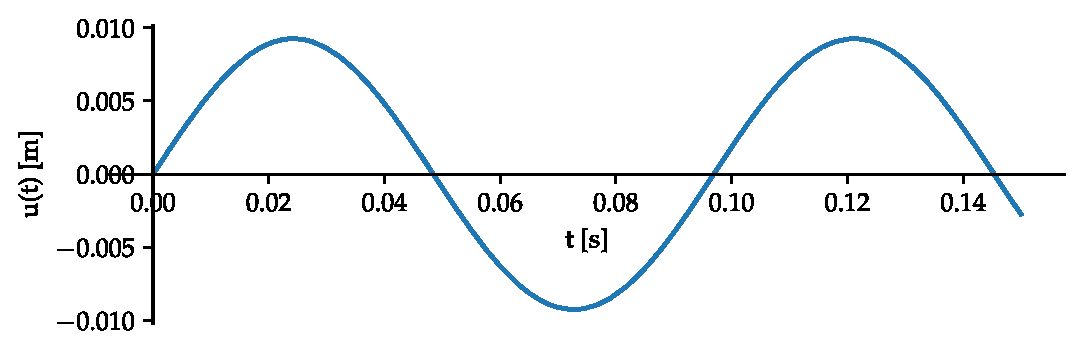
\includegraphics{index_files/mediabag/ems_02_files/figure-pdf/fig-ems_impuls_bewegungsfunk-output-1.pdf}

}

\caption{\label{fig-ems_impuls_bewegungsfunk}Zeitlicher Verlauf der
Auslenkung}

\end{figure}

\hypertarget{ruxfcckstellkraft}{%
\subsection{Rückstellkraft}\label{ruxfcckstellkraft}}

Anhand der maximalen Amplitude lässt sich die maximale Rückstellkraft
für den gesamten Rahmen bestimmen.

\begin{equation}\protect\hypertarget{eq-ems_impuls_rueckstellkraft}{}{
F_R = k   u = k   A
}\label{eq-ems_impuls_rueckstellkraft}\end{equation}

\begin{equation}u_{max} = A\end{equation}

\begin{equation}A = 0.00925 \text{m}\end{equation}

\begin{equation}F_{R} = 1.95 \cdot 10^{5} \text{N}\end{equation}

\hypertarget{spannungsnachweis}{%
\subsubsection{Spannungsnachweis}\label{spannungsnachweis}}

Die Rückstellkraft wirkt im Zentrum der Masse und bewirkt das maximale
Biegemoment bei den Fusspunkten.

\begin{figure}[H]

{\centering 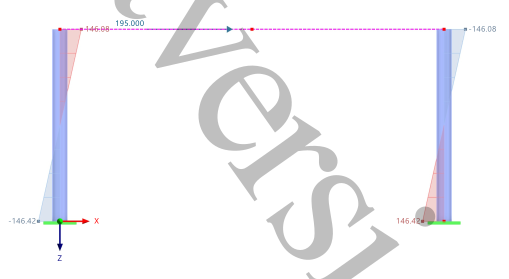
\includegraphics{bilder/impulssatz_momentenverlauf.pdf}

}

\caption{Biegemomentenverlauf durch die statische Ersatzkraft}

\end{figure}

\begin{equation}M_{max} = \frac{F_{R} H}{4}\end{equation}

\begin{equation}M_{max} = 1.46 \cdot 10^{5} \text{m} \text{N}\end{equation}

\begin{equation}\sigma_{max} = \frac{M_{max}}{W_{el y}}\end{equation}

\begin{equation}\sigma_{max} = \frac{156.0 \text{N}}{\text{mm}^{2}}\end{equation}

\begin{equation}\text{Nachweis} = \frac{156.0 \text{N}}{\text{mm}^{2}} < f_{y}\end{equation}

\begin{equation}\text{Nachweis} = \text{True}\end{equation}

\hypertarget{beispiel-dynamischer-vergruxf6sserungsfaktor}{%
\chapter{Beispiel: Dynamischer
Vergrösserungsfaktor}\label{beispiel-dynamischer-vergruxf6sserungsfaktor}}

\hypertarget{aufgabenstellung-5}{%
\section{Aufgabenstellung}\label{aufgabenstellung-5}}

Das System in Abbildung~\ref{fig-ems_dyn_verg_system_biegetrager} zeigt
einen Biegeträger, gelagert als einfacher Balken mit einer Auskragung.
Dieser wird am Kragarm mit der dynamischen Last F(t) in vertikaler
Richtung beansprucht.

\begin{figure}[H]

{\centering 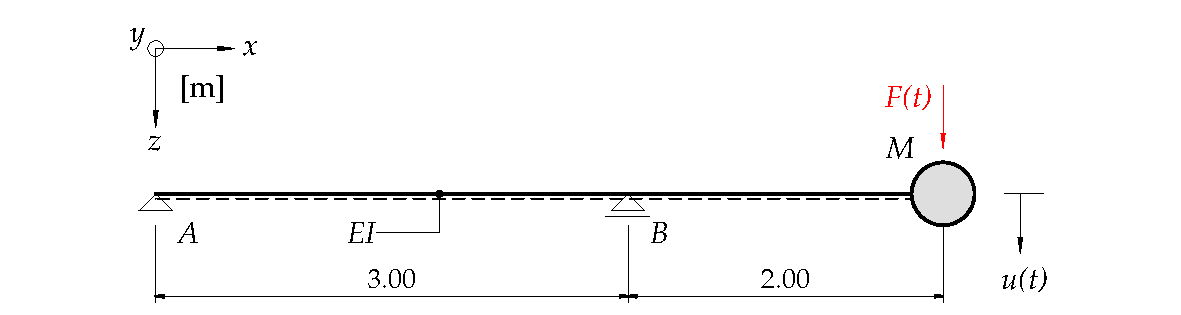
\includegraphics{index_files/mediabag/bilder/aufgabe_ems_dynamischer_vergroesserungsfaktor.pdf}

}

\caption{\label{fig-ems_dyn_verg_system_biegetrager}Statisches System
des Biegeträgers}

\end{figure}

Gesucht:

\begin{itemize}
\tightlist
\item
  Eigenkreisfrequenz \(\omega\)
\item
  Dynamischer Vergrösserungsfaktor \(V(\omega)\)
\item
  Maximale dynamische Amplitude im stationären Fall \(u_{max}\)
\end{itemize}

Gegeben:

\begin{itemize}
\tightlist
\item
  Biegeträger ist masselos
\item
  Es sind lediglich Biegeverformungen zu betrachten
  \(G \cdot A = \infty\)
  \begin{equation}\protect\hypertarget{eq-ems_dyn_verg_anregung_dynamischer_faktor}{}{
  F(t) = F_0 \cdot \cos(\omega \cdot t) = 50 \text{kN} \cdot \cos(62.8 \cdot t)
  }\label{eq-ems_dyn_verg_anregung_dynamischer_faktor}\end{equation}
\end{itemize}

\hypertarget{tbl-parameter_vergroess}{}
\begin{longtable}[]{@{}
  >{\raggedright\arraybackslash}p{(\columnwidth - 2\tabcolsep) * \real{0.5000}}
  >{\raggedright\arraybackslash}p{(\columnwidth - 2\tabcolsep) * \real{0.5000}}@{}}
\caption{\label{tbl-parameter_vergroess}Parameter der
Aufgabenstellung}\tabularnewline
\toprule\noalign{}
\endfirsthead
\endhead
\bottomrule\noalign{}
\endlastfoot
\(EI = 30000000 \text{m}^{2} \text{N}\) & \(F_{0} = 50000 \text{N}\) \\
\(l_{1} = 3000 \text{mm}\) & \(l_{2} = 2000 \text{mm}\) \\
\(m_{} = \frac{1000 \text{N} \text{s}^{2}}{\text{m}}\) &
\(\omega = \frac{62.8}{\text{s}}\) \\
\(\zeta = 0.005\) & \\
\end{longtable}

\newpage{}

\hypertarget{musterluxf6sung-3}{%
\section{Musterlösung}\label{musterluxf6sung-3}}

\hypertarget{eigenkreisfrequenz-2}{%
\subsection{Eigenkreisfrequenz}\label{eigenkreisfrequenz-2}}

Die Eigenkreisfrequenz lässt sich aus der folgenden Gleichung bestimmen:

\begin{equation}\protect\hypertarget{eq-ems_dyn_verg_eigenkreisfreq}{}{
\omega_n = \sqrt{\frac{k}{m}}
}\label{eq-ems_dyn_verg_eigenkreisfreq}\end{equation}

\hypertarget{steifigkeit-des-systems}{%
\subsubsection{Steifigkeit des Systems}\label{steifigkeit-des-systems}}

Die Steifigkeit des Systems lässt sich anhand der statischen Deformation
bestimmen. Sie entspricht dem Verhältnis zwischen Einwirkung und der
daraus resultierenden Verformung.
\begin{equation}\protect\hypertarget{eq-ems_dyn_verg_statdef}{}{
k = \frac{F}{u}
}\label{eq-ems_dyn_verg_statdef}\end{equation}

Händisch lässt sich die Deformation mittels realem und virtuellem
Kräftezustand, anhand der Arbeitsgleichung bestimmen. Dargestellt in
Abbildung~\ref{fig-ems_dyn_verg_arbeitssatz}. Die Ermittlung der
Steifigkeit bedingt lediglich das Verhältnis zwischen Einwirkung und
Deformation, folglich darf Betrag der realen Kraft frei gewählt werden.

\begin{figure}[H]

{\centering 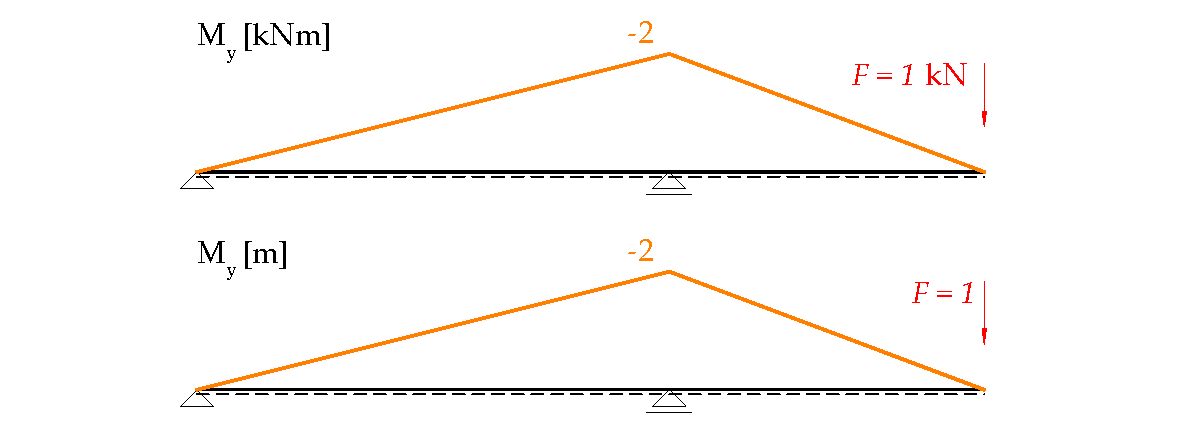
\includegraphics{index_files/mediabag/bilder/aufgabe_ems_dynamischer_vergroesserungsfaktor_my_my_fik.pdf}

}

\caption{\label{fig-ems_dyn_verg_arbeitssatz}Realer und virtueller
Kräftezustand}

\end{figure}

Um lediglich Biegeverformungen zu berücksichtigen, kann die Verformung
nach folgender Gleichung bestimmt werden.

\begin{equation}\protect\hypertarget{eq-ems_dyn_verg_deformation}{}{
u = \frac{1}{E I_y} \cdot \int_{0}^{l_1+l_2} M_y\bar{M_y} \,dx
}\label{eq-ems_dyn_verg_deformation}\end{equation}

\begin{equation}u = \frac{4000 \left(l_{1} + l_{2}\right) \text{m}^{2} \text{N}}{3 EI}\end{equation}

\begin{equation}u = 0.222 \text{mm}\end{equation}

\begin{equation}k = \frac{3 EI}{4 \left(l_{1} + l_{2}\right) \text{m}^{2}}\end{equation}

\begin{equation}k = \frac{4500 \text{N}}{\text{mm}}\end{equation}

\hypertarget{eigenkreisfrequenz-3}{%
\subsubsection{Eigenkreisfrequenz}\label{eigenkreisfrequenz-3}}

\begin{equation}\omega_{n} = \frac{\sqrt{3} \sqrt{\frac{EI}{m_{} \left(l_{1} + l_{2}\right)}}}{2 \text{m}}\end{equation}

\begin{equation}\omega_{n} = \frac{67.1}{\text{s}}\end{equation}

\hypertarget{vergruxf6sserungsfaktor}{%
\subsection{Vergrösserungsfaktor}\label{vergruxf6sserungsfaktor}}

Der Vergrösserungsfaktor beschreibt das Verhältnis zwischen der
maximalen statischen Amplitude und der maximalen dynamischen Amplitude:

\[V(\omega) = \frac{u_{max}}{u_0}\]

Dieser lässt sich mit der Dämpfungsrate \(\zeta\), Anregungsfrequenz
\(\omega\) und der Eigenfrequenz \(\omega_n\) beschreiben.

\begin{figure}[H]

{\centering 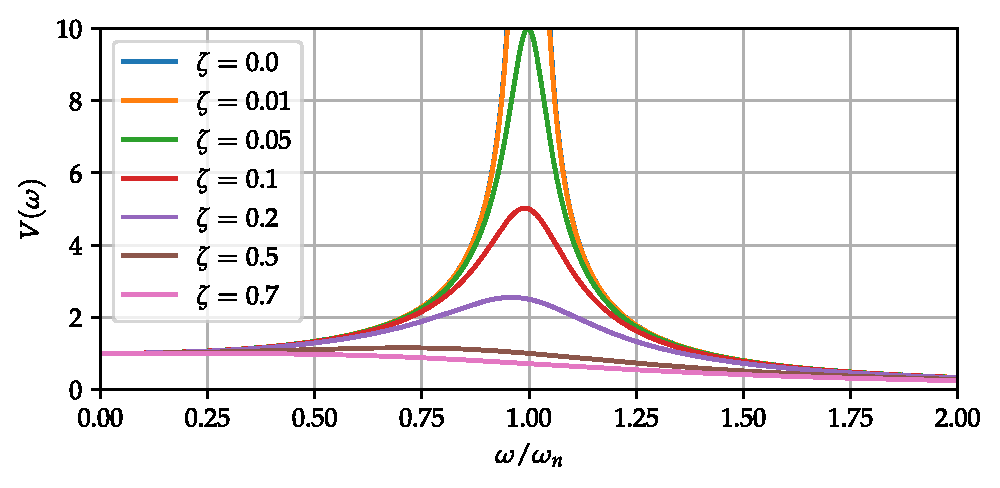
\includegraphics{index_files/mediabag/ems_03_files/figure-pdf/fig-ems_dyn_verg_vergroesserungsfaktor-output-1.pdf}

}

\caption{\label{fig-ems_dyn_verg_vergroesserungsfaktor}Einfluss der
Dämpfung und der Anregungsfrequenz auf den Vergrösserungsfaktor}

\end{figure}

\begin{equation}V{\left(\omega \right)} = \frac{1}{\sqrt{\frac{4 \omega^{2} \zeta_{}^{2}}{\omega_{n}^{2}} + \left(- \frac{\omega^{2}}{\omega_{n}^{2}} + 1\right)^{2}}}\end{equation}

\begin{equation}V{\left(\omega \right)} = 8.07\end{equation}

\hypertarget{statische-amplitude}{%
\subsection{Statische Amplitude}\label{statische-amplitude}}

Die Einwirkung lässt sich aus der Anregungsfunktion
Gleichung~\ref{eq-ems_dyn_verg_anregung_dynamischer_faktor} bestimmen
für \(t=0\). Mit der bekannten Systemsteifigkeit bestimmt sich die
Deformation.

\begin{equation}u_{stat} = \frac{F_{0}}{k}\end{equation}

\begin{equation}u_{stat} = \frac{4 F_{0} \left(l_{1} + l_{2}\right) \text{m}^{2}}{3 EI}\end{equation}

\begin{equation}u_{stat} = 11.11 \text{mm}\end{equation}

\hypertarget{stationuxe4re-amplitude}{%
\subsubsection{Stationäre Amplitude}\label{stationuxe4re-amplitude}}

Durch die Vergrösserung der statischen Deformation mit dem
Vergrösserungsfaktor resultiert die maximale Amplitude der stationären
Lösung.

\begin{equation}u_{dyn} = u_{stat} V{\left(\omega \right)}\end{equation}

\begin{equation}u_{dyn} = \frac{4 F_{0} \left(l_{1} + l_{2}\right) \text{m}^{2}}{3 EI \sqrt{\frac{16 m_{} \omega^{2} \zeta^{2} \left(l_{1} + l_{2}\right) \text{m}^{2}}{3 EI} + \left(- \frac{4 m_{} \omega^{2} \left(l_{1} + l_{2}\right) \text{m}^{2}}{3 EI} + 1\right)^{2}}}\end{equation}

\begin{equation}u_{dyn} = 89.6 \text{mm}\end{equation}

Der Nachweis der Gebrauchstauglichkeit wäre damit sicherlich nicht
erfüllt. Das Beispiel soll aufzeigen, wenn die Erregerfrequenz im
Bereich der Eigenfrequenz zu liegen kommt, es zu grossen Amplifikationen
der Verformungen bzw. zu Resonanzeffekten kommen kann.

Da meist die Masse und die Erregung (z.B. Maschine) gegeben ist, kann
man zum Beispiel ein Dämpfungselement einbauen, was jedoch keinen
wesentlichen Einfluss auf das Frequenzverhältnis hat. Dadurch werden
jedoch die Amplituden begrenzt.

Eine weitere Möglichkeit wäre die Biegesteifigkeit \(E\cdot I\) zu
erhöhen. Das System wird steifer und die Eigenfrequenz grösser. Man
spricht in dem Fall von einer Hochabstimmung.

\begin{figure}[H]

{\centering 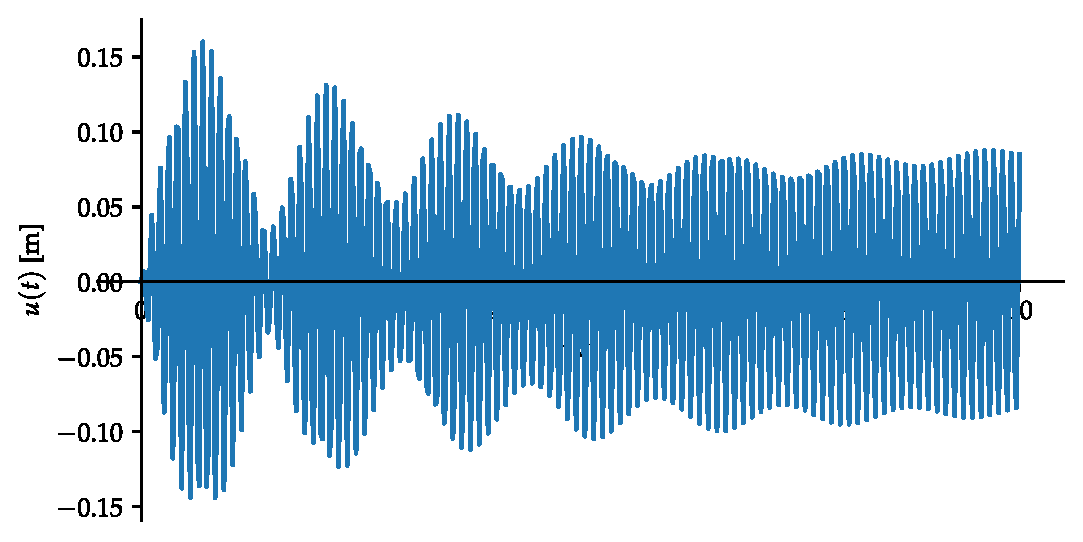
\includegraphics{index_files/mediabag/ems_03_files/figure-pdf/fig-ems_dyn_verg_gesamtantwort-output-1.pdf}

}

\caption{\label{fig-ems_dyn_verg_gesamtantwort}Gesamtantwort des
Systems}

\end{figure}

In der Abbildung~\ref{fig-ems_dyn_verg_gesamtantwort} ist die
Gesamtantwort des Systems dargestellt. Wenn Dämpfung im System vorhanden
ist, dann verschwindet die transiente bzw. homogene Lösung \(u(t)\) und
das System schwingt mit der stationären Lösung bzw. partikulären Lösung
\(u(t)\) in der Anregungsfrequenz. In Bezug auf die
Abbildung~\ref{fig-ems_dyn_verg_gesamtantwort} schwingt das System am
Anfang stärker, durch das Abklingen der Anfangsauslenkung durch die
Dämpfung schwingt das System nur noch in der Anregungsfrequenz weiter.
Die Anregung zwingt dem System seine Schwingung auf. In der Praxis sind
die Anlaufphasen zu beachten, solange der transiente Teil noch nicht
abgeklungen ist. Dort sind die Amplituden grösser und es gilt zu
untersuchen, ob diese kurzfristige Überschreitung Konsequenzen (z.B.
zul. Verformungen oder Bauteilspannungen) für das Tragsystem hat.

\hypertarget{beispiel-gesamtantwort-ohne-duxe4mpfung}{%
\chapter{Beispiel: Gesamtantwort ohne
Dämpfung}\label{beispiel-gesamtantwort-ohne-duxe4mpfung}}

\hypertarget{aufgabenstellung-6}{%
\section{Aufgabenstellung}\label{aufgabenstellung-6}}

Das System in Abbildung~\ref{fig-ems_ges_system_maschine} zeigt ein
Stabwerk, welches durch eine Werkzeugmaschine angeregt wird.

\begin{figure}[H]

{\centering 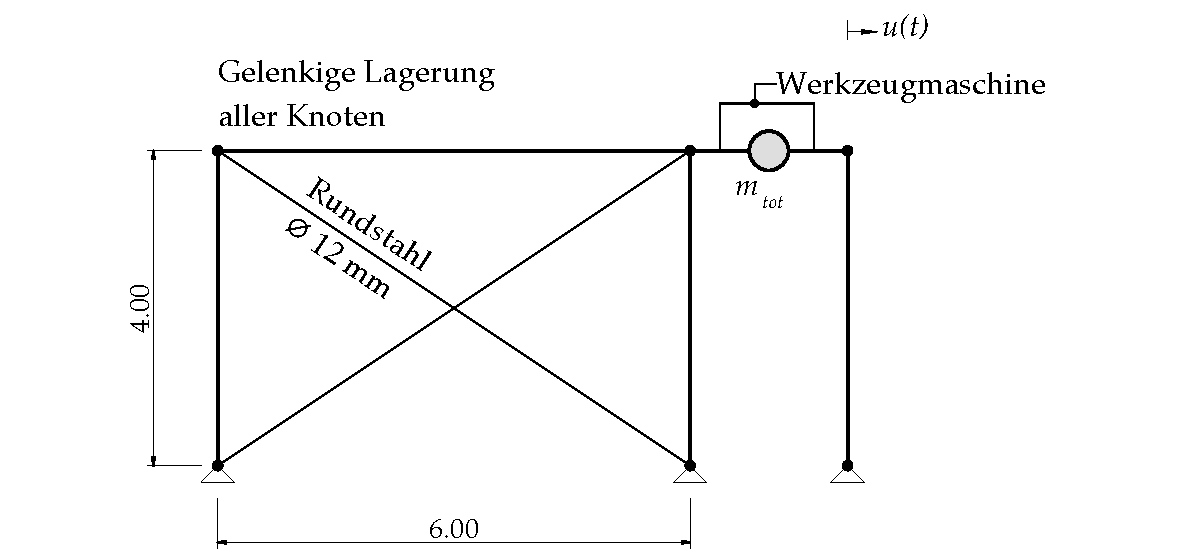
\includegraphics{index_files/mediabag/bilder/aufgabe_ems_ges_system.pdf}

}

\caption{\label{fig-ems_ges_system_maschine}Statisches System des
Stabwerks}

\end{figure}

Gesucht:

\begin{itemize}
\tightlist
\item
  Eigenkreisfrequenz \(\omega_n\)
\item
  Dynamischer Vergrösserungsfaktor \(V(\omega)\)
\item
  Stationäre Antwort \(u_p(t)\) mit dem dynamischen Vergrösserungsfaktor
  \(V(\omega)\)
\item
  Gesamtantwort \(u(t)\) mit den Anfangsbedingungen
  \(u(t=0) = 0 \text{ und } u'(t=0)=0\)
\item
  Festigkeitsnachweis der Diagonalen
\end{itemize}

Gegeben:

\begin{itemize}
\tightlist
\item
  Alle Stäbe ausser Diagonalen \(E\cdot A = \infty\)
\item
  Alle Stäbe S355
\end{itemize}

\begin{figure}[H]

{\centering 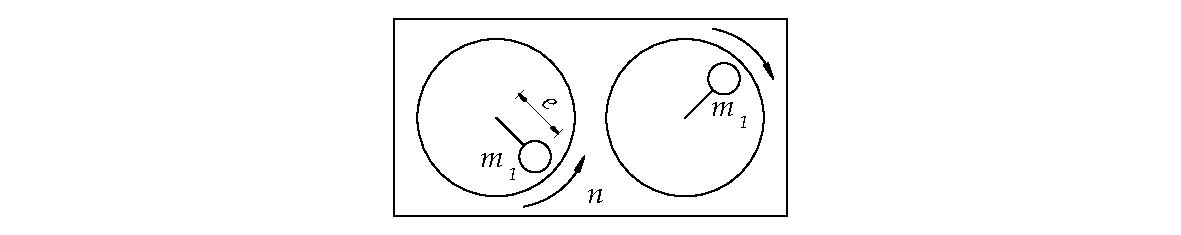
\includegraphics{index_files/mediabag/bilder/aufgabe_ems_werkzeugmaschine.pdf}

}

\caption{\label{fig-ems_ges_maschine}Aufbau der Werkzeugmaschine}

\end{figure}

\hypertarget{tbl-parameter_gesamt}{}
\begin{longtable}[]{@{}
  >{\raggedright\arraybackslash}p{(\columnwidth - 2\tabcolsep) * \real{0.5000}}
  >{\raggedright\arraybackslash}p{(\columnwidth - 2\tabcolsep) * \real{0.5000}}@{}}
\caption{\label{tbl-parameter_gesamt}Parameter der
Aufgabenstellung}\tabularnewline
\toprule\noalign{}
\endfirsthead
\endhead
\bottomrule\noalign{}
\endlastfoot
\(B = 6000 \text{mm}\) &
\(E = \frac{210000 \text{N}}{\text{mm}^{2}}\) \\
\(H = 4000 \text{mm}\) & \(\oslash_{Diag} = 12 \text{mm}\) \\
\(e = 0.1 \text{m}\) &
\(f_{yd} = \frac{338 \text{N}}{\text{mm}^{2}}\) \\
\(m_{1} = \frac{200 \text{N} \text{s}^{2}}{\text{m}}\) &
\(m_{tot} = \frac{5000 \text{N} \text{s}^{2}}{\text{m}}\) \\
\(n = \frac{150}{\text{minute}}\) & \(\zeta = 0.0\) \\
\end{longtable}

\newpage{}

\hypertarget{musterluxf6sung-4}{%
\section{Musterlösung}\label{musterluxf6sung-4}}

\hypertarget{systemsteifigkeit}{%
\subsection{Systemsteifigkeit}\label{systemsteifigkeit}}

Zur Ermittlung der Eigenkreisfrequenz wird die Steifigkeit des gesamten
Systems benötigt.

\begin{figure}[H]

{\centering 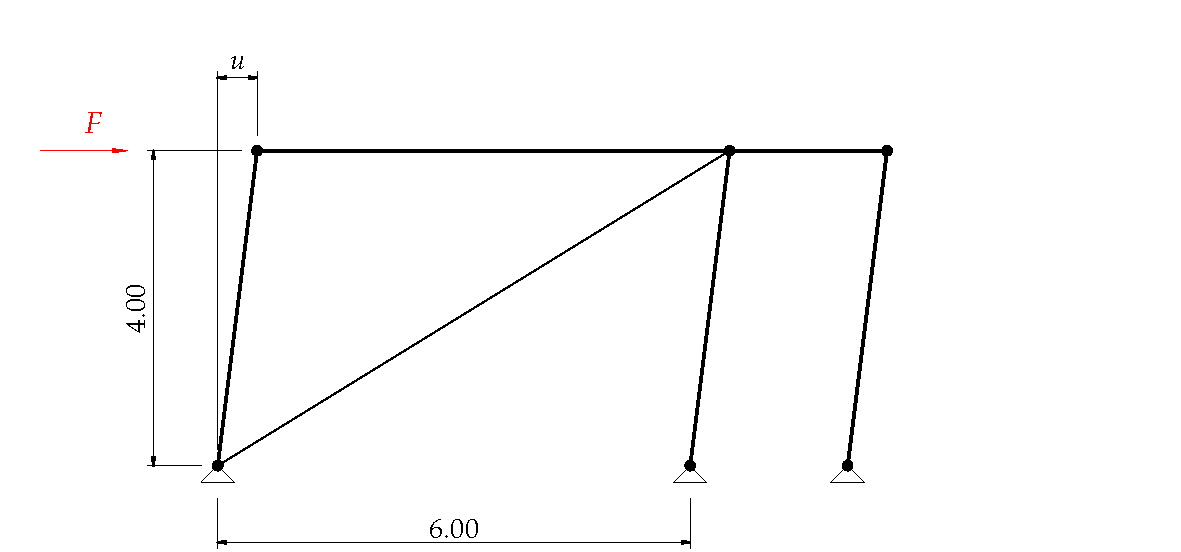
\includegraphics{index_files/mediabag/bilder/aufgabe_ems_ge_verformung.pdf}

}

\caption{\label{fig-ems_ges_verform_FW}Verformungszustand des Systems
für die Einheitskraft}

\end{figure}

Das System wird mit einer Einheitskraft belastet. Aufgrund der
Eigenschaften der Pendelstäbe (lediglich Normalkräfte) und deren
unendlich grossen Dehnsteifigkeit, spielt lediglich die Verformung der
Diagonalen eine Rolle. Dazu gilt, dass die Diagonalen nur Zugkräfte
aufnehmen können. Das bedeutet, dass letztlich ein Stab aktiv ist für
die beschrieben Situation in Abbildung~\ref{fig-ems_ges_verform_FW}.

Dazu muss die Normalkraft in der Diagonalen bestimmt werden.

\begin{equation}\alpha = \operatorname{atan}{\left(\frac{H}{B} \right)}\end{equation}

\begin{equation}\alpha = 0.588\end{equation}

\begin{equation}Z_{Diag} = 1000 \sqrt{1 + \frac{H^{2}}{B^{2}}} \text{N}\end{equation}

\begin{equation}Z_{Diag} = 1.2 \cdot 10^{3} \text{N}\end{equation}

Mittels der Arbeitsgleichung lässt sich die Verformung bestimmen. Für
die Integration zweier Normalkraftverläufe gilt die folgende Beziehung:

\begin{equation}\protect\hypertarget{eq-ems_ges_deformation}{}{
u = \frac{1}{EA_{Diag}}  \int_{0}^{l_{Diag}} N_x\bar{N_x} \,dx
}\label{eq-ems_ges_deformation}\end{equation}

Länge der Diagonalen:

\begin{equation}l_{Diag} = B \sqrt{1 + \frac{H^{2}}{B^{2}}}\end{equation}

\begin{equation}l_{Diag} = 7.21 \text{m}\end{equation}

Querschnittsfläche der Diagonalen:

\begin{equation}A_{Diag} = \frac{\pi \oslash_{Diag}^{2}}{4}\end{equation}

\begin{equation}A_{Diag} = 113.0 \text{mm}^{2}\end{equation}

Deformation der Diagonalen

\begin{equation}u_{k} = \frac{4000 B \left(1 + \frac{H^{2}}{B^{2}}\right)^{\frac{3}{2}} \text{N}}{\pi E \oslash_{Diag}^{2}}\end{equation}

\begin{equation}u_{k} = 0.439 \text{mm}\end{equation}

Steifigkeit des Systems:

\begin{equation}k = \frac{F}{u_{k}}\end{equation}

\begin{equation}k = \frac{2.28 \cdot 10^{3} \text{N}}{\text{mm}}\end{equation}

\hypertarget{eigenkreisfrequenz-4}{%
\subsection{Eigenkreisfrequenz}\label{eigenkreisfrequenz-4}}

Aus der Systemsteifigkeit lässt sich leicht die Eigenkreisfrequenz
bestimmen:

\begin{equation}\protect\hypertarget{eq-ems_ges_eigenkreisfrequenz}{}{
\omega_n =\sqrt{\frac{k}{m}}
}\label{eq-ems_ges_eigenkreisfrequenz}\end{equation}

\begin{equation}\omega_{n} = \frac{\sqrt{\pi} \sqrt{\frac{E \oslash_{Diag}^{2}}{B m_{tot} \left(1 + \frac{H^{2}}{B^{2}}\right)^{\frac{3}{2}}}}}{2}\end{equation}

\begin{equation}\omega_{n} = \frac{21.4}{\text{s}}\end{equation}

\hypertarget{dynamischer-vergruxf6sserungsfaktor}{%
\subsection{Dynamischer
Vergrösserungsfaktor}\label{dynamischer-vergruxf6sserungsfaktor}}

\hypertarget{anregungsfunktion}{%
\subsubsection{Anregungsfunktion}\label{anregungsfunktion}}

Zur Bestimmung des dynamischen Vergrösserungsfaktor wird die stationäre
Verformung benötigt. Diese lässt sich aus der Anfangskraft der
Anregungsfunktion ermitteln. Dazu wird diese Funktion benötigt. Wir
wissen die Drehzahl \(n\) und die Exzentrizität \(e\) sowie deren Masse
\(m_1\).

\begin{equation}f = n\end{equation}

\begin{equation}f = \frac{2.5}{\text{s}}\end{equation}

\begin{equation}\omega = 2 \pi f\end{equation}

\begin{equation}\omega = \frac{15.7}{\text{s}}\end{equation}

Nun fehlt lediglich die Anfangskraft \(F_0\). Die Fliehkraft \(F\) der 2
gegenläufig rotierenden Massen bewirken eine addierende Fliehkraft in
horizontaler Richtung zu:

\begin{equation}\protect\hypertarget{eq-ems_ges_anfangskraft}{}{
F_0 = 2(m_1 \cdot e \cdot \omega^2)
}\label{eq-ems_ges_anfangskraft}\end{equation}

\begin{equation}F_{0} = \frac{50 \pi^{2} e m_{1}}{\text{s}^{2}}\end{equation}

\begin{equation}F_{0} = 9.87 \cdot 10^{3} \text{N}\end{equation}

\hypertarget{statische-deformation}{%
\subsubsection{Statische Deformation}\label{statische-deformation}}

Die statische Deformation lässt sich nun leicht anhand der ermittelten
Systemsteifigkeit herleiten.

\begin{equation}u_{0} = \frac{F_{0}}{k}\end{equation}

\begin{equation}u_{0} = 4.33 \text{mm}\end{equation}

\hypertarget{vergruxf6sserungsfaktor-1}{%
\subsubsection{Vergrösserungsfaktor}\label{vergruxf6sserungsfaktor-1}}

\begin{equation}V{\left(\omega \right)} = \frac{1}{\sqrt{\frac{4 \omega^{2} \zeta_{}^{2}}{\omega_{n}^{2}} + \left(- \frac{\omega^{2}}{\omega_{n}^{2}} + 1\right)^{2}}}\end{equation}

\begin{equation}V{\left(\omega \right)} = 2.18\end{equation}

\hypertarget{stationuxe4re-antwort}{%
\subsection{Stationäre Antwort}\label{stationuxe4re-antwort}}

Es handelt sich um einen ungedämpften Einmassenschwinger mit einer
harmonischen Anregungsfunktion. Die Bewegungsgleichung ist die folgende:

\begin{equation}\protect\hypertarget{eq-ems_ges_bewegungsgleichung_inhom}{}{
mu''(t)+ ku(t) = F(t)
}\label{eq-ems_ges_bewegungsgleichung_inhom}\end{equation}

Dies ist eine inhomogene Differentialgleichung 2. Ordnung. Die Lösung
dieser lässt sich in einen partikulären Anteil und in einen homogenen
Anteil aufteilen. Der partikuläre Anteil entspricht der stationären
Antwort. Der homogene Anteil nennt sich transienter Anteil. Wäre eine
Dämpfung im System vorhanden, so startet der Schwungvorgang aus einer
Kombination beider Teile. Aufgrund der Dämpfung verschwindet der
stationäre Anteil und das System wird schlussendlich nur noch durch den
transienten Anteil deformiert.

Anhand des Vergrösserungsfaktor kann die stationäre dynamische Antwort
des Systems mit der folgenden Beziehung ermittelt werden.

\begin{equation}\protect\hypertarget{eq-ems_ges_part_loesung}{}{
u_p = V(\omega)u_0 \cdot \cos{(\omega t)}
}\label{eq-ems_ges_part_loesung}\end{equation}

\begin{equation}u_{p} = 9.43 \cos{\left(\frac{5 \pi t}{\text{s}} \right)} \text{mm}\end{equation}

\hypertarget{gesamtantwort}{%
\subsection{Gesamtantwort}\label{gesamtantwort}}

Für die Gesamtantwort wird nun noch der homogene Anteil benötigt. Dazu
ist die folgende Differentialgleichung zu lösen.

\begin{equation}\protect\hypertarget{eq-ems_ges_bewegungsgleichung_homog}{}{
mu''(t)+ ku(t) = 0
}\label{eq-ems_ges_bewegungsgleichung_homog}\end{equation}

Als Ansatzfunktion dient die folgende Gleichung:

\begin{equation}\protect\hypertarget{eq-ems_ges_ansatz_homogen}{}{
u_h = A_1\cos{(\omega_n t)} + A_2 \sin{(\omega_n t)}
}\label{eq-ems_ges_ansatz_homogen}\end{equation}

Die Randbedingungen sind in der Aufgabenstellung definiert und sind die
folgenden:

\(u(t=0)=0\)

\(u'(t=0)=0\)

Vorsicht, die Randbedingungen gelten für die gesamte Lösung:

\begin{equation}\protect\hypertarget{eq-ems_ges_gesamtloesung}{}{
u(t) = u_h(t) + u_p(t)
}\label{eq-ems_ges_gesamtloesung}\end{equation}

\begin{figure}[H]

{\centering 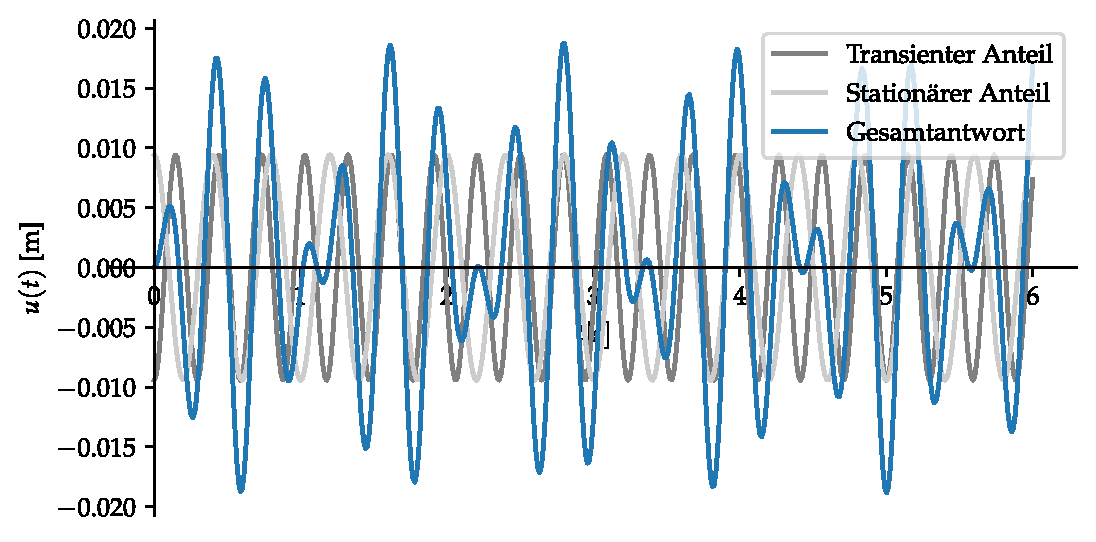
\includegraphics{index_files/mediabag/ems_04_files/figure-pdf/fig-ems_ges_gesamtantwort_ems4-output-1.pdf}

}

\caption{\label{fig-ems_ges_gesamtantwort_ems4}Antworten des Systems
ohne Dämpfung}

\end{figure}

\hypertarget{festigkeitsnachweis}{%
\subsection{Festigkeitsnachweis}\label{festigkeitsnachweis}}

Aufgrund der maximalen Auslenkung, kann die maximale Normalkraft auf der
Diagonalen bestimmt werden.

\hypertarget{maximale-auslenkung}{%
\subsubsection{Maximale Auslenkung}\label{maximale-auslenkung}}

Aus dem Plot in Abbildung~\ref{fig-ems_ges_gesamtantwort_ems4} ist die
maximale Auslenkung ersichtlich. Die Ermittlung des Zeitpunkts bei einer
maximalen Auslenkung wird hier numerisch gelöst.

\begin{equation}t_{max} = 2.8 \text{s}\end{equation}

\begin{equation}u_{max} = 0.0188 \text{m}\end{equation}

\hypertarget{maximale-einwirkung}{%
\subsubsection{Maximale Einwirkung}\label{maximale-einwirkung}}

Aufgrund der maximalen Amplitude verlängert sich die Diagonale um
\(\Delta l = u_{max}\). Die Dehnung des Stabs ist somit die
\(\frac{\Delta l}{l_{Diag}}\). Bei linear elastischem Materialverhalten
gilt die folgende Beziehung:

\begin{equation}\protect\hypertarget{eq-ems_ges_spannung}{}{
\sigma = \varepsilon E
}\label{eq-ems_ges_spannung}\end{equation}

\begin{equation}\varepsilon = 0.00314\end{equation}

\begin{equation}\sigma = \frac{659.0 \text{N}}{\text{mm}^{2}}\end{equation}

\begin{equation}f_{yd} = \frac{338 \text{N}}{\text{mm}^{2}}\end{equation}

\begin{equation}Nachweis = \frac{\sigma}{f_{yd}}\end{equation}

\begin{equation}Nachweis = 1.95\end{equation}

Die Diagonale würde plastifizieren, so dass die linearen Annahmen für
die Berechnung der Systemantwort nicht angewendet werden dürfen.

\hypertarget{beispiel-gesamtantwort-mit-duxe4mpfung}{%
\chapter{Beispiel: Gesamtantwort mit
Dämpfung}\label{beispiel-gesamtantwort-mit-duxe4mpfung}}

\hypertarget{aufgabenstellung-7}{%
\section{Aufgabenstellung}\label{aufgabenstellung-7}}

Das System in Abbildung~\ref{fig-ems_dampf_system} entspricht dem System
in Abbildung~\ref{fig-ems_ges_system_maschine}. Ergänzt wurde dies mit
einem Dämpfungselement.

\begin{figure}[H]

{\centering 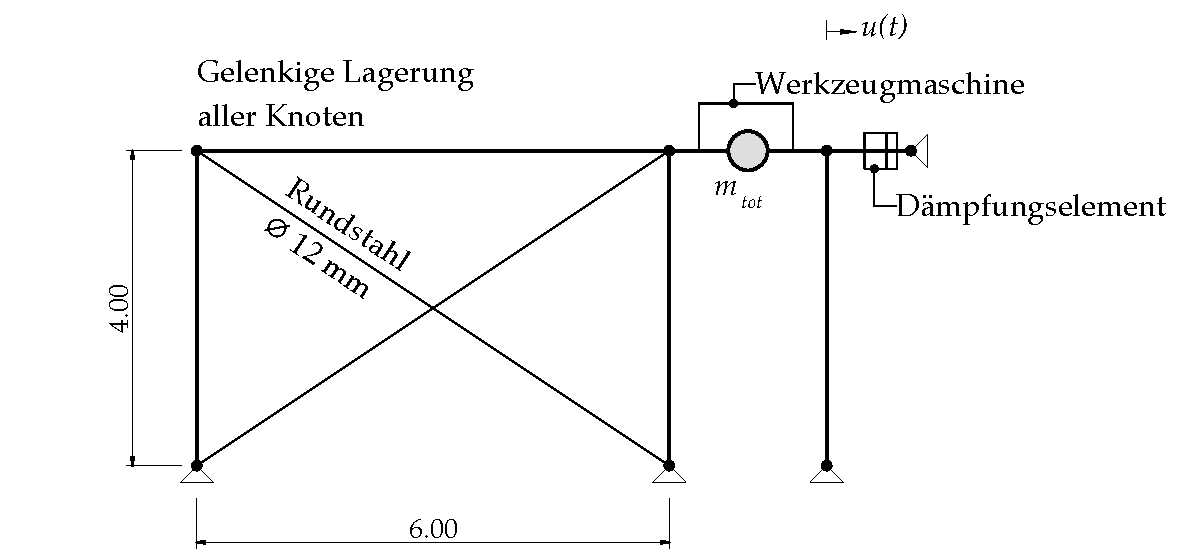
\includegraphics{index_files/mediabag/bilder/aufgabe_ems_gedampft_system.pdf}

}

\caption{\label{fig-ems_dampf_system}Statisches System}

\end{figure}

Gesucht:

\begin{itemize}
\tightlist
\item
  Dynamischer Vergrösserungsfaktor \(V(\omega)\)
\item
  Stationäre Amplitude
\item
  Festigkeitsnachweis der Diagonalen
\end{itemize}

Gegeben:

\begin{itemize}
\tightlist
\item
  Alle Stäbe ausser Diagonalen \(E\cdot A = \infty\)
\item
  Alle Stäbe S355
\end{itemize}

\begin{figure}[H]

{\centering 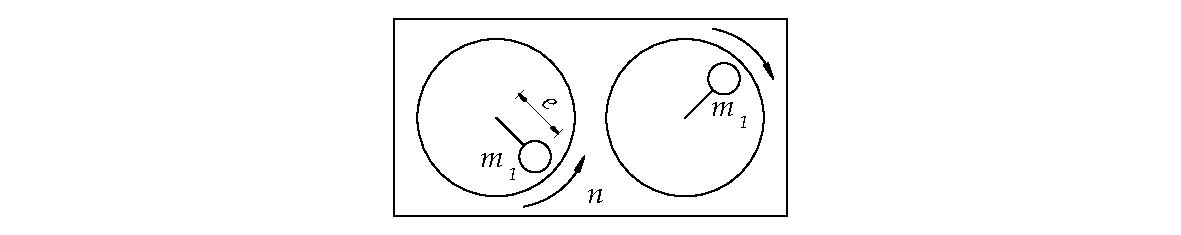
\includegraphics{index_files/mediabag/bilder/aufgabe_ems_werkzeugmaschine.pdf}

}

\caption{\label{fig-ems_ges_maschine}Aufbau der Werkzeugmaschine}

\end{figure}

\hypertarget{tbl-parameter_gesamt_dampf}{}
\begin{longtable}[]{@{}
  >{\raggedright\arraybackslash}p{(\columnwidth - 2\tabcolsep) * \real{0.5000}}
  >{\raggedright\arraybackslash}p{(\columnwidth - 2\tabcolsep) * \real{0.5000}}@{}}
\caption{\label{tbl-parameter_gesamt_dampf}Parameter der
Aufgabenstellung}\tabularnewline
\toprule\noalign{}
\endfirsthead
\endhead
\bottomrule\noalign{}
\endlastfoot
\(B = 6000 \text{mm}\) &
\(E = \frac{210000 \text{N}}{\text{mm}^{2}}\) \\
\(H = 4000 \text{mm}\) & \(\oslash_{Diag} = 12 \text{mm}\) \\
\(e = 0.1 \text{m}\) &
\(f_{yd} = \frac{338 \text{N}}{\text{mm}^{2}}\) \\
\(m_{1} = \frac{200 \text{N} \text{s}^{2}}{\text{m}}\) &
\(m_{tot} = \frac{5000 \text{N} \text{s}^{2}}{\text{m}}\) \\
\(n = \frac{150}{\text{minute}}\) & \(\zeta = 0.2\) \\
\end{longtable}

\newpage{}

\hypertarget{musterluxf6sung-5}{%
\section{Musterlösung}\label{musterluxf6sung-5}}

\hypertarget{systemsteifigkeit-1}{%
\subsection{Systemsteifigkeit}\label{systemsteifigkeit-1}}

Zur Ermittlung der Eigenkreisfrequenz wird die Steifigkeit des gesamten
Systems benötigt.

\begin{figure}[H]

{\centering 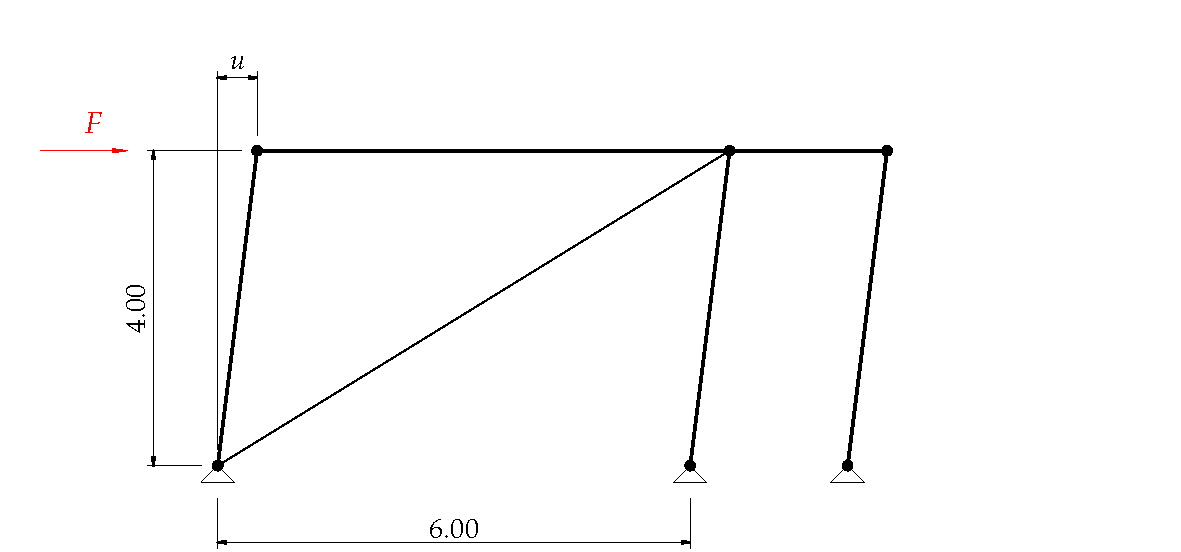
\includegraphics{index_files/mediabag/bilder/aufgabe_ems_ge_verformung.pdf}

}

\caption{\label{fig-ems_dampf_verform_FW}Verformungszustand des Systems
für die Einheitskraft}

\end{figure}

Das System wird mit einer Einheitskraft belastet. Aufgrund der
Eigenschaften der Pendelstäbe (lediglich Normalkräfte) und deren
unendlich grossen Dehnsteifigkeit, spielt lediglich die Verformung der
Diagonalen eine Rolle. Dazu gilt, dass die Diagonalen nur Zugkräfte
aufnehmen können. Das bedeutet, dass letztlich ein Stab aktiv ist für
die beschrieben Situation in Abbildung~\ref{fig-ems_dampf_verform_FW}.

Dazu muss die Normalkraft in der Diagonalen bestimmt werden.

\begin{equation}\alpha = \operatorname{atan}{\left(\frac{H}{B} \right)}\end{equation}

\begin{equation}\alpha = 0.588\end{equation}

\begin{equation}Z_{Diag} = 1000 \sqrt{1 + \frac{H^{2}}{B^{2}}} \text{N}\end{equation}

\begin{equation}Z_{Diag} = 1.2 \cdot 10^{3} \text{N}\end{equation}

Mittels der Arbeitsgleichung lässt sich die Verformung bestimmen. Für
die Integration zweier Normalkraftverläufe gilt die folgende Beziehung:

\begin{equation}\protect\hypertarget{eq-ems_dampf_deformation}{}{
u = \frac{1}{EA_{Diag}}  \int_{0}^{l_{Diag}} N_x\bar{N_x} \,dx
}\label{eq-ems_dampf_deformation}\end{equation}

Länge der Diagonalen:

\begin{equation}l_{Diag} = B \sqrt{1 + \frac{H^{2}}{B^{2}}}\end{equation}

\begin{equation}l_{Diag} = 7.21 \text{m}\end{equation}

Querschnittsfläche der Diagonalen:

\begin{equation}A_{Diag} = \frac{\pi \oslash_{Diag}^{2}}{4}\end{equation}

\begin{equation}A_{Diag} = 113.0 \text{mm}^{2}\end{equation}

Deformation der Diagonalen

\begin{equation}u_{k} = \frac{4000 B \left(1 + \frac{H^{2}}{B^{2}}\right)^{\frac{3}{2}} \text{N}}{\pi E \oslash_{Diag}^{2}}\end{equation}

\begin{equation}u_{k} = 0.439 \text{mm}\end{equation}

Steifigkeit des Systems:

\begin{equation}k = \frac{F}{u_{k}}\end{equation}

\begin{equation}k = \frac{2.28 \cdot 10^{3} \text{N}}{\text{mm}}\end{equation}

\hypertarget{eigenkreisfrequenz-5}{%
\subsection{Eigenkreisfrequenz}\label{eigenkreisfrequenz-5}}

Aus der Systemsteifigkeit lässt sich leicht die Eigenkreisfrequenz
bestimmen:

\begin{equation}\protect\hypertarget{eq-ems_dampf_eigenkreisfrequenz}{}{
\omega_n =\sqrt{\frac{k}{m}}
}\label{eq-ems_dampf_eigenkreisfrequenz}\end{equation}

\begin{equation}\omega_{n} = \frac{\sqrt{\pi} \sqrt{\frac{E \oslash_{Diag}^{2}}{B m_{tot} \left(1 + \frac{H^{2}}{B^{2}}\right)^{\frac{3}{2}}}}}{2}\end{equation}

\begin{equation}\omega_{n} = \frac{21.4}{\text{s}}\end{equation}

\hypertarget{dynamischer-vergruxf6sserungsfaktor-1}{%
\subsection{Dynamischer
Vergrösserungsfaktor}\label{dynamischer-vergruxf6sserungsfaktor-1}}

\hypertarget{anregungsfunktion-1}{%
\subsubsection{Anregungsfunktion}\label{anregungsfunktion-1}}

Zur Bestimmung des dynamischen Vergrösserungsfaktor wird die stationäre
Verformung benötigt. Diese lässt sich aus der Anfangskraft der
Anregungsfunktion ermitteln. Dazu wird diese Funktion benötigt. Wir
wissen die Drehzahl \(n\) und die Exzentrizität \(e\) sowie deren Masse
\(m_1\).

\begin{equation}f = n\end{equation}

\begin{equation}f = \frac{2.5}{\text{s}}\end{equation}

\begin{equation}\omega = 2 \pi f\end{equation}

\begin{equation}\omega = \frac{15.7}{\text{s}}\end{equation}

Nun fehlt lediglich die Anfangskraft \(F_0\). Die Fliehkraft \(F\) der 2
gegenläufig rotierenden Massen bewirken eine addierende Fliehkraft in
horizontaler Richtung zu:

\begin{equation}\protect\hypertarget{eq-ems_dampf_anfangskraft}{}{
F_0 = 2(m_1 \cdot e \cdot \omega^2)
}\label{eq-ems_dampf_anfangskraft}\end{equation}

\begin{equation}F_{0} = \frac{50 \pi^{2} e m_{1}}{\text{s}^{2}}\end{equation}

\begin{equation}F_{0} = 9.87 \cdot 10^{3} \text{N}\end{equation}

\hypertarget{statische-deformation-1}{%
\subsubsection{Statische Deformation}\label{statische-deformation-1}}

Die statische Deformation lässt sich nun leicht anhand der ermittelten
Systemsteifigkeit herleiten.

\begin{equation}u_{0} = 4.33 \text{mm}\end{equation}

\hypertarget{vergruxf6sserungsfaktor-2}{%
\subsubsection{Vergrösserungsfaktor}\label{vergruxf6sserungsfaktor-2}}

\begin{equation}V{\left(\omega \right)} = \frac{1}{\sqrt{\frac{4 \omega^{2} \zeta_{}^{2}}{\omega_{n}^{2}} + \left(- \frac{\omega^{2}}{\omega_{n}^{2}} + 1\right)^{2}}}\end{equation}

\begin{equation}V{\left(\omega \right)} = 1.83\end{equation}

\hypertarget{stationuxe4re-antwort-1}{%
\subsection{Stationäre Antwort}\label{stationuxe4re-antwort-1}}

Es handelt sich um einen gedämpften Einmassenschwinger mit einer
harmonischen Anregungsfunktion. Die Bewegungsgleichung ist die folgende:

\begin{equation}\protect\hypertarget{eq-ems_dampf_bewegungsgleichung_inhomo}{}{
mu''(t)+ cu'(t) + ku(t) = F(t)
}\label{eq-ems_dampf_bewegungsgleichung_inhomo}\end{equation}

Dies ist eine inhomogene Differentialgleichung 2. Ordnung. Die Lösung
dieser lässt sich in einen partikulären Anteil und in einen homogenen
Anteil aufteilen. Der partikuläre Anteil entspricht der stationären
Antwort. Der homogene Anteil nennt sich transienter Anteil.

Anhand des Vergrösserungsfaktor kann die stationäre dynamische Antwort
des Systems mit der folgenden Beziehung ermittelt werden.

\begin{equation}\protect\hypertarget{eq-ems_dampf_part_loesung}{}{
u_p = V(\omega)u_0 \cdot \cos{(\omega t)}
}\label{eq-ems_dampf_part_loesung}\end{equation}

\begin{equation}u_{p} = 0.00793 \cos{\left(\frac{5 \pi t}{\text{s}} \right)} \text{m}\end{equation}

\hypertarget{gesamtantwort-1}{%
\subsection{Gesamtantwort}\label{gesamtantwort-1}}

Für die Gesamtantwort wird nun noch der homogene Anteil benötigt. Dazu
ist die folgende Differentialgleichung zu lösen.

\begin{equation}\protect\hypertarget{eq-ems_dampf_bewegungsgleichung_homo}{}{
mu''(t)+ cu'(t) + ku(t) = 0
}\label{eq-ems_dampf_bewegungsgleichung_homo}\end{equation}

Als Ansatzfunktion dient die folgende Gleichung:

\begin{equation}\protect\hypertarget{eq-ems_dampf_homo_loesung}{}{
u_h = e^{-\zeta \omega_n t} (A_1\cos{(\omega_d t)} + A_2 \sin{(\omega_d t)})
}\label{eq-ems_dampf_homo_loesung}\end{equation}

Die Randbedingungen sind in der Aufgabenstellung definiert und sind die
folgenden:

\(u(t=0)=0\)

\(u'(t=0)=0\)

Vorsicht, die Randbedingungen gelten für die gesamte Lösung:

\begin{equation}\protect\hypertarget{eq-ems_dampf_gesamtloesung}{}{
u(t) = u_h(t) + u_p(t)
}\label{eq-ems_dampf_gesamtloesung}\end{equation}

\hypertarget{geduxe4mpfte-eigenkreisfrequenz}{%
\subsubsection{Gedämpfte
Eigenkreisfrequenz}\label{geduxe4mpfte-eigenkreisfrequenz}}

\begin{equation}\omega_{d} = \omega_{n} \sqrt{1 - \zeta_{}^{2}}\end{equation}

\begin{equation}\omega_{d} = \frac{20.9}{\text{s}}\end{equation}

\begin{figure}[H]

{\centering 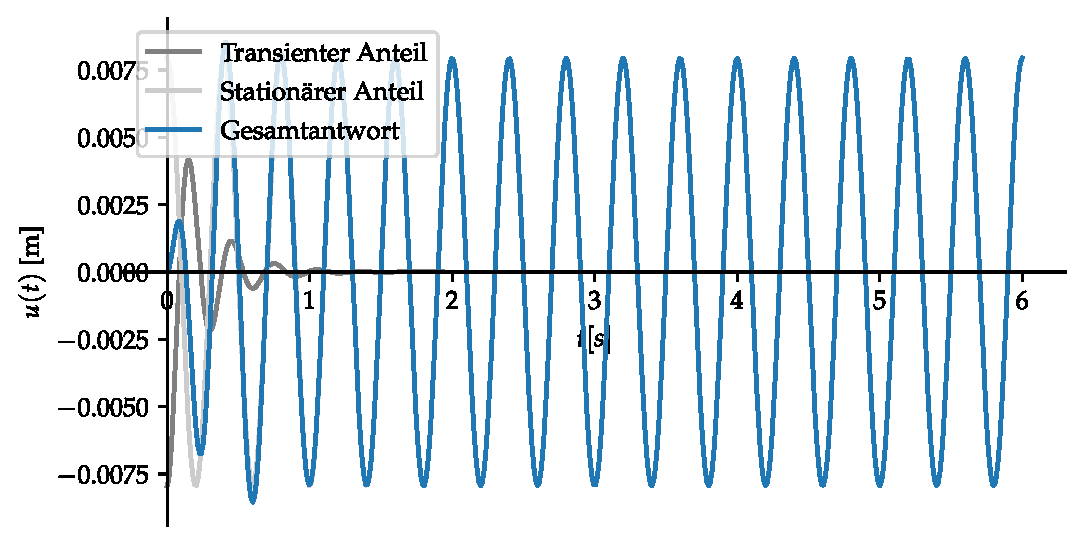
\includegraphics{index_files/mediabag/ems_05_files/figure-pdf/fig-ems_dampf_gesamtantwort_ems5-output-1.pdf}

}

\caption{\label{fig-ems_dampf_gesamtantwort_ems5}Gesamtantwort des
Systems}

\end{figure}

\hypertarget{festigkeitsnachweis-1}{%
\subsection{Festigkeitsnachweis}\label{festigkeitsnachweis-1}}

Aufgrund der maximalen Auslenkung, kann die maximale Normalkraft auf der
Diagonalen bestimmt werden.

\hypertarget{maximale-auslenkung-1}{%
\subsubsection{Maximale Auslenkung}\label{maximale-auslenkung-1}}

Aus dem Plot in Abbildung~\ref{fig-ems_dampf_gesamtantwort_ems5} ist die
maximale Auslenkung ersichtlich. Die Ermittlung des Zeitpunkts bei einer
maximalen Auslenkung wird hier numerisch gelöst.

\begin{equation}t_{max} = 0.41 \text{s}\end{equation}

\begin{equation}u_{max} = 0.00855 \text{m}\end{equation}

\hypertarget{maximale-einwirkung-1}{%
\subsubsection{Maximale Einwirkung}\label{maximale-einwirkung-1}}

Aufgrund der maximalen Amplitude verlängert sich die Diagonale um
\(\Delta l=u_{max}\). Die Dehnung des Stabs ist somit die
\(\frac{\Delta l}{l_{Diag}}\). Bei linear elastischem Materialverhalten
gilt die folgende Beziehung:

\begin{equation}\protect\hypertarget{eq-ems_dampf_spannung}{}{
\sigma = \varepsilon E
}\label{eq-ems_dampf_spannung}\end{equation}

\begin{equation}\varepsilon = 0.00142\end{equation}

\begin{equation}\sigma = \frac{299.0 \text{N}}{\text{mm}^{2}}\end{equation}

\begin{equation}f_{yd} = \frac{338 \text{N}}{\text{mm}^{2}}\end{equation}

\begin{equation}Nachweis = \frac{\sigma}{f_{yd}}\end{equation}

\begin{equation}Nachweis = 0.885\end{equation}

Die Diagonale bleibt im elastichen Bereich, so dass die linearen
Annahmen gültig sind. Der Festigkeitsnachweis für die Diagonale ist
erfüllt. Im Weiteren wäre der Grenzustand der Tragfähigkeit
\emph{Ermüdung} zu prüfen.

\hypertarget{beispiel-fourier-transformation}{%
\chapter{Beispiel:
Fourier-Transformation}\label{beispiel-fourier-transformation}}

\hypertarget{aufgabenstellung-8}{%
\section{Aufgabenstellung}\label{aufgabenstellung-8}}

Nachfolgend ist ein unterspannter Träger gezeigt, der durch eine
periodische Rechteckanregung dynamisch beansprucht wird.

\begin{figure}[H]

{\centering 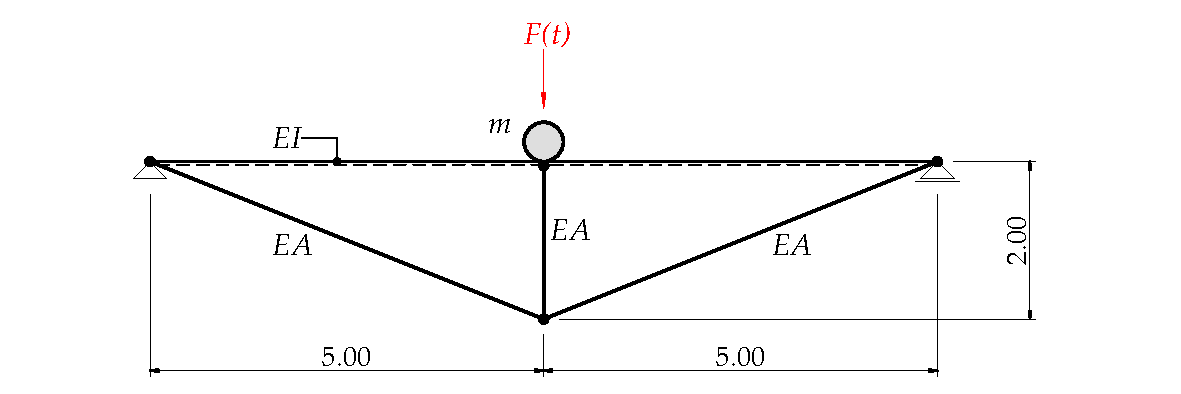
\includegraphics{index_files/mediabag/bilder/aufgabe_ems_fourier_system.pdf}

}

\caption{\label{fig-ems-fourier_system}Statisches System des
unterspannten Trägers}

\end{figure}

Gesucht:

\begin{itemize}
\tightlist
\item
  Eigenkreisfrequenz \(\omega_n\)
\item
  Stationäre Amplitude der Verschiebung
\item
  Staionäre Amplitude der Beschleunigung
\end{itemize}

Gegeben:

\begin{itemize}
\tightlist
\item
  Rechteckanregung in Abbildung~\ref{fig-ems-fourier_rechteckanregung}
\end{itemize}

\hypertarget{tbl-parameter_fourier}{}
\begin{longtable}[]{@{}
  >{\raggedright\arraybackslash}p{(\columnwidth - 2\tabcolsep) * \real{0.5000}}
  >{\raggedright\arraybackslash}p{(\columnwidth - 2\tabcolsep) * \real{0.5000}}@{}}
\caption{\label{tbl-parameter_fourier}Parameter der
Aufgabenstellung}\tabularnewline
\toprule\noalign{}
\endfirsthead
\endhead
\bottomrule\noalign{}
\endlastfoot
\(A = 1000 \text{N}\) & \(A_{Fachwerk} = 3000 \text{mm}^{2}\) \\
\(E = \frac{200000 \text{N}}{\text{mm}^{2}}\) &
\(I_{Balken} = 200000000 \text{mm}^{4}\) \\
\(h = 2 \text{m}\) & \(l = 5 \text{m}\) \\
\(m_{} = \frac{1000 \text{N} \text{s}^{2}}{\text{m}}\) &
\(\zeta = 0.0\) \\
\end{longtable}

\begin{figure}[H]

{\centering 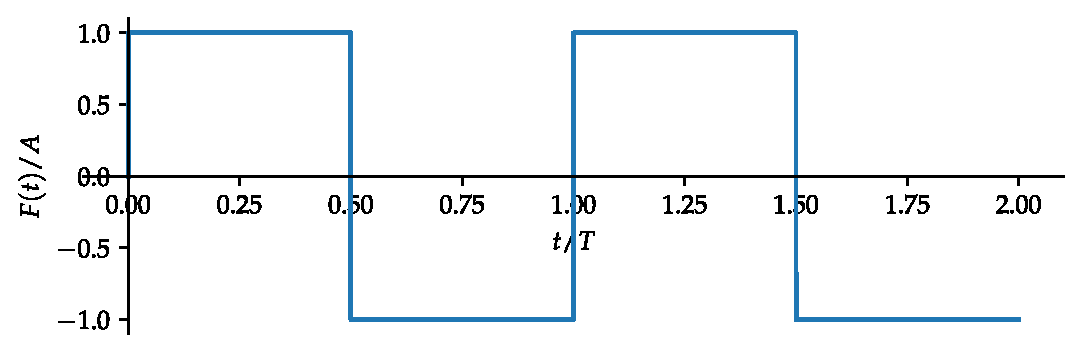
\includegraphics{index_files/mediabag/ems_06_files/figure-pdf/fig-ems-fourier_rechteckanregung-output-1.pdf}

}

\caption{\label{fig-ems-fourier_rechteckanregung}Rechteckige
Anregungsfunktion}

\end{figure}

\newpage{}

\hypertarget{musterluxf6sung-6}{%
\section{Musterlösung}\label{musterluxf6sung-6}}

\hypertarget{erregerfunktion}{%
\subsection{Erregerfunktion}\label{erregerfunktion}}

Die periodische Erregerfunktion wird mit einer Fourier-Reihenentwicklung
approximiert um eine periodisch, harmonische Funktion zu generieren.

Die Reihenentwicklung folgt folgender Funktion:

\begin{equation}\protect\hypertarget{eq-ems_fourier_reihe}{}{
F(t) = A_0 + \sum_{n=1}^{\infty}(a_n\cdot \cos{(n\omega t)}+b_n \cdot \sin{(n\omega t)})
}\label{eq-ems_fourier_reihe}\end{equation}

Die Aufgabenstellung fordert lediglich die ersten drei Teile der Reihe.

\begin{equation}\protect\hypertarget{eq-ems_fourier_3_terme}{}{
F(t) = A_0 + \sum_{n=1}^{3}(a_n \cdot \cos{(n\omega t)}+b_n \cdot \sin{(n\omega t)})
}\label{eq-ems_fourier_3_terme}\end{equation}

Nach Bestimmung der Konstanten folgt die Gleichung zu:

\begin{equation}\protect\hypertarget{eq-ems_fourier_geloest}{}{
F(t) = \frac{4A}{\pi} \cdot [\sin(\omega t) + \frac{1}{3}\sin(3\omega t) + \frac{1}{5}\sin(5 \omega t)]
}\label{eq-ems_fourier_geloest}\end{equation}

\begin{equation}f_{Anregung} = \frac{1}{\text{s}}\end{equation}

\begin{equation}\omega = \frac{6.28}{\text{s}}\end{equation}

\begin{equation}F{\left(t \right)} = \frac{4 A \left(\sin{\left(\frac{2 \pi t}{\text{s}} \right)} + \frac{\sin{\left(\frac{6 \pi t}{\text{s}} \right)}}{3} + \frac{\sin{\left(\frac{10 \pi t}{\text{s}} \right)}}{5}\right)}{\pi}\end{equation}

\begin{figure}[H]

{\centering 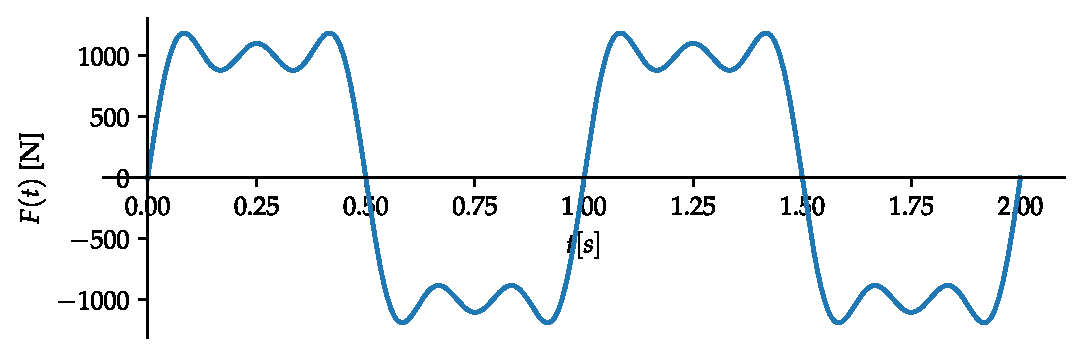
\includegraphics{index_files/mediabag/ems_06_files/figure-pdf/cell-8-output-1.pdf}

}

\end{figure}

\hypertarget{systemsteifigkeit-2}{%
\subsection{Systemsteifigkeit}\label{systemsteifigkeit-2}}

Anhand der Arbeitsgleichung wird die Deformation bestimmt und daraus die
Steifigkeit des Systems. Auf die Bestimmung der Schnittgrössen wird
nicht eingegangen. Es handelt sich um ein statisch unbestimmtes System.

\begin{figure}[H]

{\centering 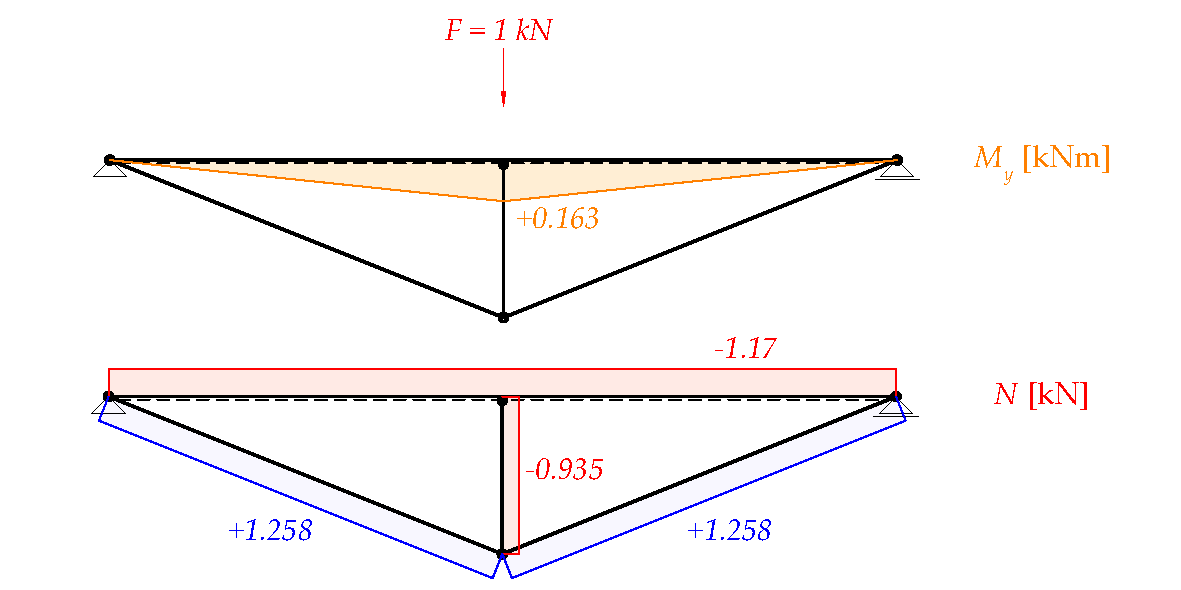
\includegraphics{index_files/mediabag/bilder/aufgabe_ems_fourier_schnittgroessen.pdf}

}

\caption{\label{fig-ems-fourier_schnittgroessen_real}Schnittgrössen des
unterspannten Balkens}

\end{figure}

\begin{figure}[H]

{\centering 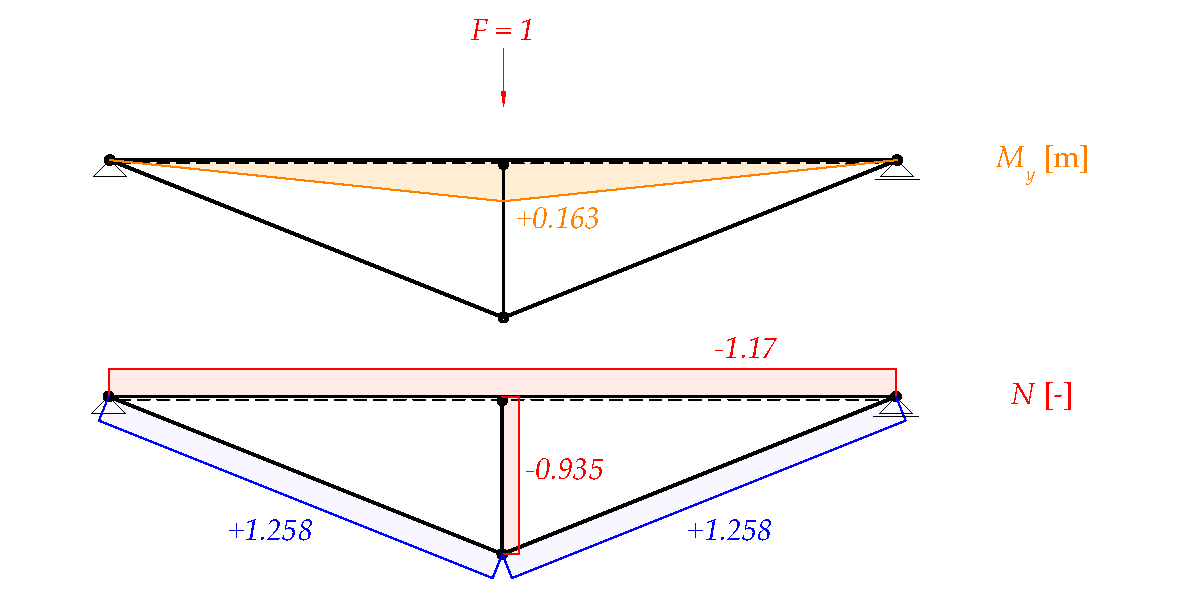
\includegraphics{index_files/mediabag/bilder/aufgabe_ems_fourier_schnittgroessen_fikt.pdf}

}

\caption{\label{fig-ems-fourier_schnittgroessen_virt}Virtuelle
Schnittgrössen des unterspannten Balkens}

\end{figure}

Da der Balken dehnstarr ist und die Unterspannung aus Pendelstäben
zusammengesetzt ist, sind Anteile aus Normalkraft aus den Pendelstäben
und lediglich Anteile aus Biegung im Balken für die Deformation
zuständig.

\begin{equation}u_{k} = 0.0335 \text{mm}\end{equation}

\begin{equation}k = \frac{2.98 \cdot 10^{7} \text{N}}{\text{m}}\end{equation}

\hypertarget{eigenkreisfrequenz-6}{%
\subsection{Eigenkreisfrequenz}\label{eigenkreisfrequenz-6}}

Aus der Systemsteifigkeit lässt sich leicht die Eigenkreisfrequenz
bestimmen:

\begin{equation}\protect\hypertarget{eq-ems_fourier_eigenkreisfrequenz}{}{
\omega_n =\sqrt{\frac{k}{m}}
}\label{eq-ems_fourier_eigenkreisfrequenz}\end{equation}

\begin{equation}\omega_{n} = \frac{173.0}{\text{s}}\end{equation}

\hypertarget{stationuxe4re-amplitude-der-verschiebung}{%
\subsection{Stationäre Amplitude der
Verschiebung}\label{stationuxe4re-amplitude-der-verschiebung}}

Die statische Durchbiegung lässt sich anhand der Systemsteifigkeit und
der Anfangskraft der Anregungsfunktion bestimmen. Mittels des
Vergrösserungsfaktors lässt sich schlussendlich die stationäre maximale
Amplitude bestimmen. Der Vergrösserungsfaktor ist abhängig von der
Anregungsfrequenz, welche wir mit der Fourier-Reihenentwicklung
approximiert haben. Wir haben folglich \emph{``3 verschiedene''}
Anregungsfrequenzen mit der entsprechenden Gewichtung.

\begin{equation}V{\left(\omega \right)} = \frac{1}{5 \sqrt{\frac{100 \omega^{2} \zeta_{}^{2}}{\omega_{n}^{2}} + \left(- \frac{25 \omega^{2}}{\omega_{n}^{2}} + 1\right)^{2}}} + \frac{1}{3 \sqrt{\frac{36 \omega^{2} \zeta_{}^{2}}{\omega_{n}^{2}} + \left(- \frac{9 \omega^{2}}{\omega_{n}^{2}} + 1\right)^{2}}} + \frac{1}{\sqrt{\frac{4 \omega^{2} \zeta_{}^{2}}{\omega_{n}^{2}} + \left(- \frac{\omega^{2}}{\omega_{n}^{2}} + 1\right)^{2}}}\end{equation}

\begin{equation}V{\left(\omega \right)} = 1.55\end{equation}

\begin{equation}u_{0} = 0.0427 \text{mm}\end{equation}

\begin{equation}u_{stat} = 0.066 \text{mm}\end{equation}

Der Vergrösserungsfaktor ist erwartungsgemäss niedrig, da sich die
Eigenkreisfrequenz deutlich von der Anregungsfrequenz abgrenzt.

\hypertarget{stationuxe4re-amplitude-der-beschleunigung}{%
\subsection{Stationäre Amplitude der
Beschleunigung}\label{stationuxe4re-amplitude-der-beschleunigung}}

\ul{Die Beschleunigung lässt sich ebenfalls anhand des
Vergrösserungsfaktors bestimmen. Dies Entspricht dem Vorgehen nach
Michael Baur.}

\begin{equation}V_{a}{\left(\omega \right)} = 0.00205\end{equation}

\begin{equation}\frac{d^{2}}{d t^{2}} u_{max} = \frac{0.0026 \text{m}}{\text{s}^{2}}\end{equation}

\ul{Meines Erachtens müsste der Vergrösserungsfaktor für die
Beschleunigung ebenfalls mit sämtlichen, gewichteten Anregungsfrequenzen
der approximierten Anregungsfunktion bestimmt werden.}

\begin{equation}V_{a}{\left(\omega \right)} = 0.00614\end{equation}

\begin{equation}\frac{d^{2}}{d t^{2}} u_{max} = \frac{0.00781 \text{m}}{\text{s}^{2}}\end{equation}

\hypertarget{sec-ems_untilg}{%
\chapter{Beispiel: Balken ohne Tilger}\label{sec-ems_untilg}}

\hypertarget{aufgabenstellung-9}{%
\section{Aufgabenstellung}\label{aufgabenstellung-9}}

Ein einfacher Balken mit einer Einzelmasse, welcher in dieser Aufgabe
ohne Tilger ausgestattet ist, ist in
Abbildung~\ref{fig-ems_untilg_system_ohne_tilger} dargestellt. Die Masse
erfährt eine dynamische Einwirkung durch die Funktion \(F(t)\). Das
Beispiel wird in Kapitel~\ref{sec-tilger} weitergeführt.

\begin{figure}[H]

{\centering 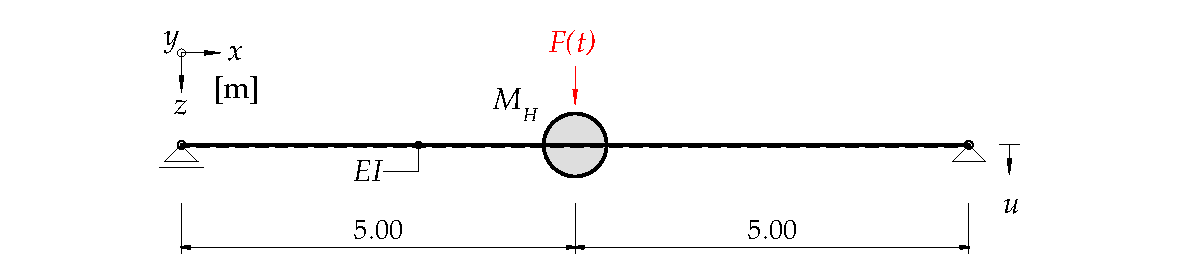
\includegraphics{index_files/mediabag/bilder/aufgabe_ems_untilg_system.pdf}

}

\caption{\label{fig-ems_untilg_system_ohne_tilger}Statisches System des
Balkens ohne Tilger}

\end{figure}

Gesucht:

\begin{itemize}
\tightlist
\item
  Maximale dynamische Verformung mittels stationärer Lösung
\item
  Maximale dynamische Beschleunigung mittels stationärer Lösung
\end{itemize}

Gegeben:

\hypertarget{tbl-parameter_mms3}{}
\begin{longtable}[]{@{}
  >{\raggedright\arraybackslash}p{(\columnwidth - 2\tabcolsep) * \real{0.5000}}
  >{\raggedright\arraybackslash}p{(\columnwidth - 2\tabcolsep) * \real{0.5000}}@{}}
\caption{\label{tbl-parameter_mms3}Parameter der
Aufgabenstellung}\tabularnewline
\toprule\noalign{}
\endfirsthead
\endhead
\bottomrule\noalign{}
\endlastfoot
\(E = \frac{200000 \text{N}}{\text{mm}^{2}}\) &
\(F_{0} = 800.0 \text{N}\) \\
\(I = 200000000 \text{mm}^{4}\) & \(L = 5 \text{m}\) \\
\(M_{H} = \frac{2000 \text{N} \text{s}^{2}}{\text{m}}\) &
\(\omega = \frac{12.6}{\text{s}}\) \\
\(\zeta = 0.0\) & \\
\end{longtable}

\[
F(t) = F_0 \cdot \sin(\omega\cdot t) = 0.8 \text{kN} \cdot (12.6 \frac{\text{rad}}{\text{s}}\cdot t)
\]

\newpage{}

\hypertarget{musterluxf6sung-7}{%
\section{Musterlösung}\label{musterluxf6sung-7}}

\hypertarget{steifigkeit-k}{%
\subsection{\texorpdfstring{Steifigkeit
\(k\)}{Steifigkeit k}}\label{steifigkeit-k}}

Zuerst wird die Steifigkeit des Systems ermittelt, für einen
Einmassenschwinger entspricht diese der Biegesteifigkeit des Balkens.

\begin{equation}k_{H} = \frac{6 E I}{L^{3}}\end{equation}

\begin{equation}k_{H} = \frac{1.92 \cdot 10^{6} \text{N}}{\text{m}}\end{equation}

\hypertarget{eigenkreisfrequenz-omega}{%
\subsection{\texorpdfstring{Eigenkreisfrequenz
\(\omega\)}{Eigenkreisfrequenz \textbackslash omega}}\label{eigenkreisfrequenz-omega}}

Die Eigekreisfrequenz kann mit der bekannten Formel ermittelt werden:

\begin{equation}\omega_{n} = \sqrt{\frac{k}{m}}\end{equation}

\begin{equation}\omega_{n} = \sqrt{6} \sqrt{\frac{E I}{L^{3} M_{H}}}\end{equation}

\begin{equation}\omega_{n} = \frac{31.0}{\text{s}}\end{equation}

\hypertarget{vergruxf6sserungsfaktor-vomega}{%
\subsection{\texorpdfstring{Vergrösserungsfaktor
\(V(\omega)\)}{Vergrösserungsfaktor V(\textbackslash omega)}}\label{vergruxf6sserungsfaktor-vomega}}

Da lediglich die Stationäre Antwort von Interesse ist, kann mittels
Vergrösserungsfaktor diese ermittelt werden. Der Verlauf entspricht der
Anregungsfunktion. Die Amplitude definiert sich aus der statischen
Deformation mit dem Vergrösserungsfaktor multipliziert.

\begin{equation}V{\left(\omega \right)} = \frac{1}{\sqrt{\frac{4 \omega^{2} \zeta_{}^{2}}{\omega_{n}^{2}} + \left(- \frac{\omega^{2}}{\omega_{n}^{2}} + 1\right)^{2}}}\end{equation}

\begin{equation}V{\left(\omega \right)} = 1.2\end{equation}

\hypertarget{stationuxe4re-luxf6sung}{%
\subsection{Stationäre Lösung}\label{stationuxe4re-luxf6sung}}

\hypertarget{statische-deformation-2}{%
\subsubsection{Statische Deformation}\label{statische-deformation-2}}

\begin{equation}u_{0} = \frac{F_{0}}{k_{H}}\end{equation}

\begin{equation}u_{0} = \frac{F_{0} L^{3}}{6 E I}\end{equation}

\begin{equation}u_{0} = 0.4167 \text{mm}\end{equation}

\hypertarget{stationuxe4re-maximale-deformation}{%
\subsubsection{Stationäre maximale
Deformation}\label{stationuxe4re-maximale-deformation}}

\begin{equation}u_{stat} = u_{0} V{\left(\omega \right)}\end{equation}

\begin{equation}u_{stat} = \frac{F_{0} L^{3}}{6 E I \sqrt{\left(1 - \frac{L^{3} M_{H} \omega^{2}}{6 E I}\right)^{2} + \frac{2 L^{3} M_{H} \omega^{2} \zeta^{2}}{3 E I}}}\end{equation}

\begin{equation}u_{stat} = 0.499 \text{mm}\end{equation}

\hypertarget{stationuxe4re-maximale-beschleunigung}{%
\subsubsection{Stationäre maximale
Beschleunigung}\label{stationuxe4re-maximale-beschleunigung}}

\begin{equation}V_{a}{\left(\omega \right)} = \frac{V_{\omega} \omega^{2}}{\omega_{n}^{2}}\end{equation}

\begin{equation}V_{a}{\left(\omega \right)} = 0.198\end{equation}

\begin{equation}\frac{d^{2}}{d t^{2}} u_{stat} = \frac{0.0793 \text{m}}{\text{s}^{2}}\end{equation}

\begin{figure}[H]

{\centering 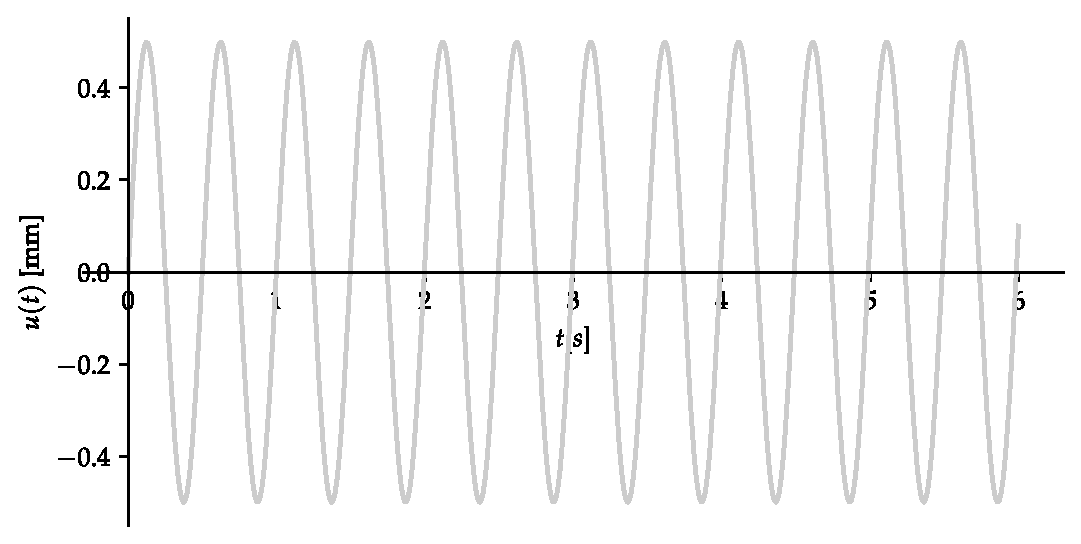
\includegraphics{index_files/mediabag/ems_07_files/figure-pdf/fig-ems_untilg_stationaer_antwort-output-1.pdf}

}

\caption{\label{fig-ems_untilg_stationaer_antwort}Stationäre Antwort des
Systems}

\end{figure}

\part{Mehrmassenschwinger}

\hypertarget{sec-mms_steif}{%
\chapter{Beispiel: Eigenvektoren mit direkt bestimmter
Steifigkeitsmatrix}\label{sec-mms_steif}}

\hypertarget{aufgabenstellung-10}{%
\section{Aufgabenstellung}\label{aufgabenstellung-10}}

Das System in Abbildung~\ref{fig-mms_steif_system_mms2} zeigt ein
Rahmentragwerk, welches als Zweimassenschwinger modelliert werden kann.

\begin{figure}[H]

{\centering 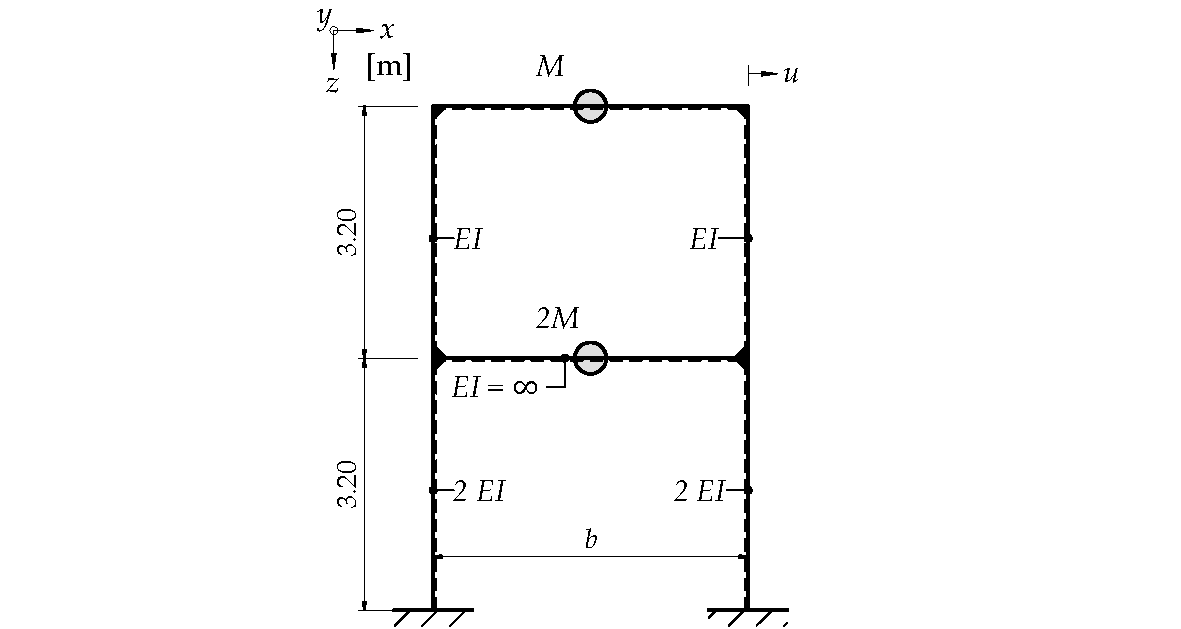
\includegraphics{index_files/mediabag/bilder/aufgabe_mms_steif_system.pdf}

}

\caption{\label{fig-mms_steif_system_mms2}Statisches System des
Rahmentragwerks}

\end{figure}

Gesucht:

\begin{itemize}
\item
  Eigenkreisfrequenz \(\omega\)
\item
  Eigenformen - Normierung auf \[\phi_1^T = 
  \begin{bmatrix}
   &  1\\
  \end{bmatrix} \] \[\phi_2^T =
  \begin{bmatrix}
   &  1\\
  \end{bmatrix}\]
\item
  Skizze der Eigenformen
\end{itemize}

Gegeben:

\begin{itemize}
\tightlist
\item
  Dehnsteifigkeit aller Stäbe \(E\cdot A = \infty\)
\end{itemize}

\hypertarget{tbl-parameter_mms2}{}
\begin{longtable}[]{@{}
  >{\raggedright\arraybackslash}p{(\columnwidth - 2\tabcolsep) * \real{0.5000}}
  >{\raggedright\arraybackslash}p{(\columnwidth - 2\tabcolsep) * \real{0.5000}}@{}}
\caption{\label{tbl-parameter_mms2}Parameter der
Aufgabenstellung}\tabularnewline
\toprule\noalign{}
\endfirsthead
\endhead
\bottomrule\noalign{}
\endlastfoot
\(E = \frac{30000 \text{N}}{\text{mm}^{2}}\) & \(H = 3.2 \text{m}\) \\
\(I = 2000000000 \text{mm}^{4}\) &
\(m_{1} = \frac{40000 \text{N} \text{s}^{2}}{\text{m}}\) \\
\(m_{2} = \frac{20000 \text{N} \text{s}^{2}}{\text{m}}\) & \\
\end{longtable}

\newpage{}

\hypertarget{sec-mms_steif_ML}{%
\section{Musterlösung}\label{sec-mms_steif_ML}}

\hypertarget{eigenkreisfrequenzen}{%
\subsection{Eigenkreisfrequenzen}\label{eigenkreisfrequenzen}}

\hypertarget{sec-mms_steif_kmatrix}{%
\subsubsection{\texorpdfstring{Steifigkeitsmatrix
\(\mathbf{K}\)}{Steifigkeitsmatrix \textbackslash mathbf\{K\}}}\label{sec-mms_steif_kmatrix}}

Zur Bestimmung der Steifigkeitsmatrix ist das System an jedem
Freiheitsgrad auszulenken, wie in
Abbildung~\ref{fig-mms_steif_steifigkeit} dargestellt ist.

\begin{figure}[H]

{\centering 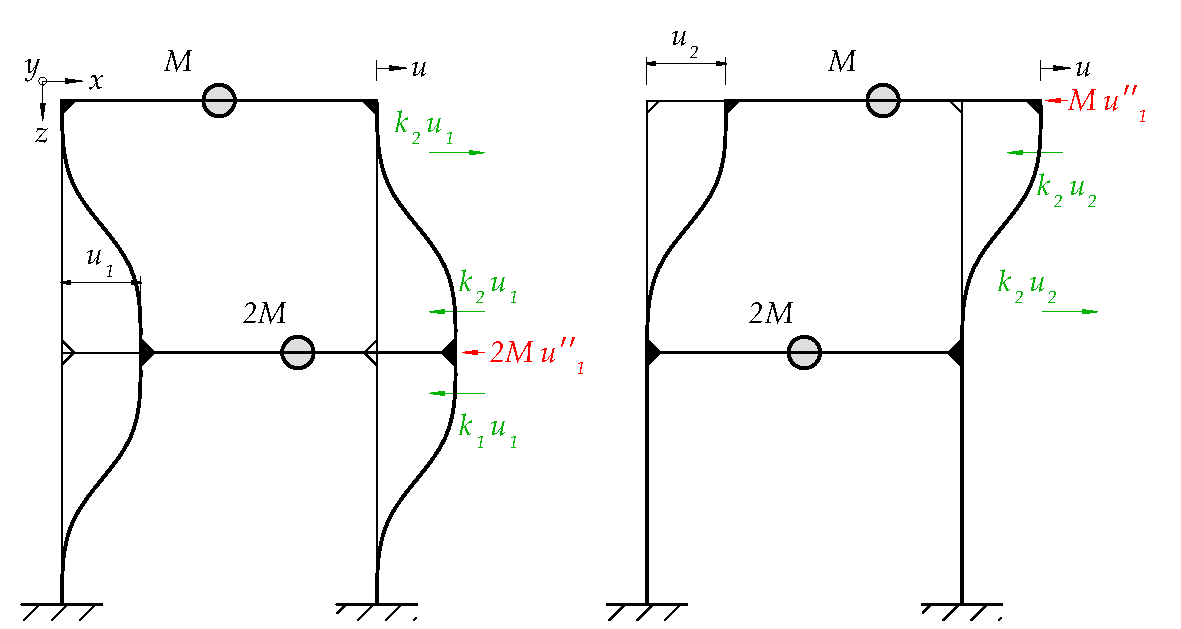
\includegraphics{index_files/mediabag/bilder/aufgabe_mms_steif_auslenk.pdf}

}

\caption{\label{fig-mms_steif_steifigkeit}Auslenkung der Freiheitsgrade
zur Bestimmung der Steifigkeit}

\end{figure}

Wichtig dabei sind die Richtungen der Kräfte. Als Denkstütze gilt
folgendes:

\begin{itemize}
\tightlist
\item
  Der Auslenkung um \(u\) wirkt die Federkraft entgegen, welche \(k u\)
  entspricht.
\item
  Zusätzlich wirkt die Trägheitskraft der Auslenkung entgegen, welche
  \(m u''\) entspricht.
\item
  Nach der Betrachtung des ausgelenkten Punkts, kann mittels
  \emph{Actio-Reactio}-Prinzip das ``\emph{Stockwerk}'' ins
  Gleichgewicht gebracht werden.
\item
  Vorzeichen sind gegen der Bewegungsrichtig positiv.
\end{itemize}

\hypertarget{horizontale-steifigkeit-2}{%
\subsubsection{Horizontale
Steifigkeit}\label{horizontale-steifigkeit-2}}

Für entsprechende Anwendungsfälle gibt es fertige Lösungen zur
Bestimmung der Steifigkeit. Gemäss
Abbildung~\ref{fig-mms_steif_system_mms2} ist die Stütze am Fuss- und
Kopfpunkt eingespannt. Somit resultiert die Steifigkeit zu:

\begin{equation}\protect\hypertarget{eq-mms_steif_steifigkeit}{}{
k_{Stuetze} = \frac{12EI_{Stuetze}}{H^3}
}\label{eq-mms_steif_steifigkeit}\end{equation}

Diese gilt für eine einzelne Stütze. Eingesetzt in die
Steifigkeitsmatrix:

\begin{equation}k_{1} = \frac{48 E I}{H^{3}}\end{equation}

\begin{equation}k_{2} = \frac{24 E I}{H^{3}}\end{equation}

\begin{equation}K = \left[\begin{matrix}k_{1} + k_{2} & - k_{2}\\- k_{2} & k_{2}\end{matrix}\right]\end{equation}

\begin{equation}K = \left[\begin{matrix}\frac{1.31836 \cdot 10^{8} \text{N}}{\text{m}} & - \frac{4.39453 \cdot 10^{7} \text{N}}{\text{m}}\\- \frac{4.39453 \cdot 10^{7} \text{N}}{\text{m}} & \frac{4.39453 \cdot 10^{7} \text{N}}{\text{m}}\end{matrix}\right]\end{equation}

\hypertarget{eigenvektoren}{%
\subsection{Eigenvektoren}\label{eigenvektoren}}

\hypertarget{massenmatrix-mathbfm}{%
\subsubsection{\texorpdfstring{Massenmatrix
\(\mathbf{M}\)}{Massenmatrix \textbackslash mathbf\{M\}}}\label{massenmatrix-mathbfm}}

Die Massenmatrix folgt dem gleichen Aufbau wie die Steifigkeitsmatrix.
Es gelten die gleichen Vorzeichenregelungen.

\begin{equation}M = \left[\begin{matrix}m_{1} & 0\\0 & m_{2}\end{matrix}\right]\end{equation}

\begin{equation}M = \left[\begin{matrix}\frac{40000 \text{N} \text{s}^{2}}{\text{m}} & 0\\0 & \frac{20000 \text{N} \text{s}^{2}}{\text{m}}\end{matrix}\right]\end{equation}

\hypertarget{eigenkreisfrequenzen-1}{%
\subsubsection{Eigenkreisfrequenzen}\label{eigenkreisfrequenzen-1}}

Bei einem Mehrmassenschwinger gibt es entsprechend den Freiheitsgraden
Eigenkreisfrequenzen \(\omega_n\). Diese lassen sich anhand folgender
Gleichung bestimmen:

\[\det{[\mathbf{K}-\omega_n^2 \mathbf{M}]=0}\]

\begin{equation}\omega_{1} = \frac{33.1}{\text{s}}\end{equation}

\begin{equation}\omega_{2} = \frac{66.3}{\text{s}}\end{equation}

\hypertarget{eigenvektoren-phi}{%
\subsubsection{\texorpdfstring{Eigenvektoren
\(\phi\)}{Eigenvektoren \textbackslash phi}}\label{eigenvektoren-phi}}

\begin{equation}\left[\begin{matrix}\frac{- k_{2} m_{2} \phi_{21} + \frac{\phi_{11} \left(- k_{2} m_{1} + m_{2} \left(k_{1} + k_{2}\right) + \sqrt{k_{1}^{2} m_{2}^{2} - 2 k_{1} k_{2} m_{1} m_{2} + 2 k_{1} k_{2} m_{2}^{2} + k_{2}^{2} m_{1}^{2} + 2 k_{2}^{2} m_{1} m_{2} + k_{2}^{2} m_{2}^{2}}\right)}{2}}{m_{2}}\\\frac{- k_{2} m_{1} \phi_{11} + \frac{\phi_{21} \left(k_{2} m_{1} - m_{2} \left(k_{1} + k_{2}\right) + \sqrt{k_{1}^{2} m_{2}^{2} - 2 k_{1} k_{2} m_{1} m_{2} + 2 k_{1} k_{2} m_{2}^{2} + k_{2}^{2} m_{1}^{2} + 2 k_{2}^{2} m_{1} m_{2} + k_{2}^{2} m_{2}^{2}}\right)}{2}}{m_{1}}\end{matrix}\right] = \left[\begin{matrix}0\\0\end{matrix}\right]\end{equation}

\begin{equation}\phi_{1} = \left[\begin{matrix}0.5\\1.0\end{matrix}\right]\end{equation}

\begin{equation}\left[\begin{matrix}\frac{- k_{2} m_{2} \phi_{22} + \frac{\phi_{12} \left(- k_{2} m_{1} + m_{2} \left(k_{1} + k_{2}\right) - \sqrt{k_{1}^{2} m_{2}^{2} - 2 k_{1} k_{2} m_{1} m_{2} + 2 k_{1} k_{2} m_{2}^{2} + k_{2}^{2} m_{1}^{2} + 2 k_{2}^{2} m_{1} m_{2} + k_{2}^{2} m_{2}^{2}}\right)}{2}}{m_{2}}\\\frac{- k_{2} m_{1} \phi_{12} + \frac{\phi_{22} \left(k_{2} m_{1} - m_{2} \left(k_{1} + k_{2}\right) - \sqrt{k_{1}^{2} m_{2}^{2} - 2 k_{1} k_{2} m_{1} m_{2} + 2 k_{1} k_{2} m_{2}^{2} + k_{2}^{2} m_{1}^{2} + 2 k_{2}^{2} m_{1} m_{2} + k_{2}^{2} m_{2}^{2}}\right)}{2}}{m_{1}}\end{matrix}\right] = \left[\begin{matrix}0\\0\end{matrix}\right]\end{equation}

\begin{equation}\phi_{2} = \left[\begin{matrix}-1.0\\1.0\end{matrix}\right]\end{equation}

\hypertarget{orthogonalituxe4tsbedingung}{%
\subsubsection{Orthogonalitätsbedingung}\label{orthogonalituxe4tsbedingung}}

Zur Entkoppelung des Systems wird die Orthogonalität der Eigenvektoren
kontrolliert. Siehe Kapitel~\ref{sec-mms_nach_ortho} für eine
ausführliche Erklärung.

\begin{equation}\phi_{1}^{T} M \phi_{1} = \left[\begin{matrix}\frac{3.0 \cdot 10^{4} \text{N} \text{s}^{2}}{\text{m}}\end{matrix}\right]\end{equation}

\begin{equation}\phi_{2}^{T} M \phi_{2} = \left[\begin{matrix}\frac{6.0 \cdot 10^{4} \text{N} \text{s}^{2}}{\text{m}}\end{matrix}\right]\end{equation}

\begin{equation}\phi_{2}^{T} M \phi_{1} = \left[\begin{matrix}0\end{matrix}\right]\end{equation}

\begin{equation}\phi_{1}^{T} M \phi_{2} = \left[\begin{matrix}0\end{matrix}\right]\end{equation}

Für die Steifigkeitsmatrix:

\begin{equation}\phi_{1}^{T} K \phi_{1} = \left[\begin{matrix}\frac{3.3 \cdot 10^{7} \text{N}}{\text{m}}\end{matrix}\right]\end{equation}

\begin{equation}\phi_{2}^{T} K \phi_{2} = \left[\begin{matrix}\frac{2.64 \cdot 10^{8} \text{N}}{\text{m}}\end{matrix}\right]\end{equation}

\begin{equation}\phi_{2}^{T} K \phi_{1} = \left[\begin{matrix}0\end{matrix}\right]\end{equation}

\begin{equation}\phi_{1}^{T} K \phi_{2} = \left[\begin{matrix}0\end{matrix}\right]\end{equation}

\hypertarget{eigenformen}{%
\subsection{Eigenformen}\label{eigenformen}}

\begin{figure}[H]

{\centering 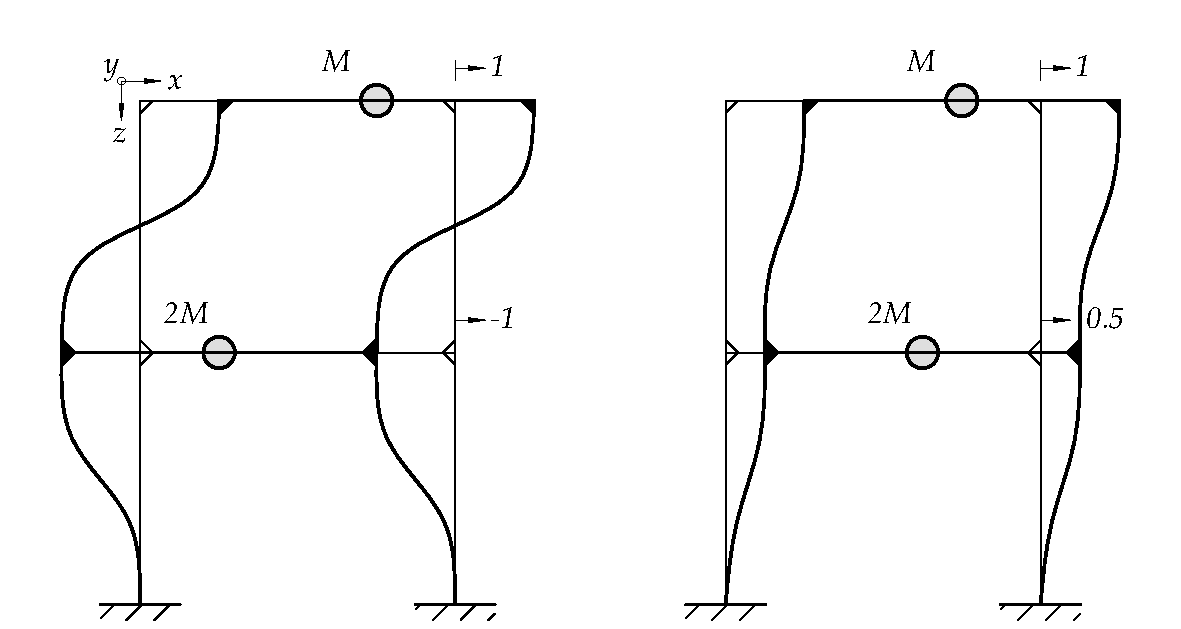
\includegraphics{index_files/mediabag/bilder/aufgabe_mms_steif_eigenvektoren.pdf}

}

\caption{\label{fig-mms_steif_eigenformen}Die beiden Eigenformen
skizziert}

\end{figure}

\hypertarget{beispiel-eigenvektoren-und-nachgiebigkeitsmatrix}{%
\chapter{Beispiel: Eigenvektoren und
Nachgiebigkeitsmatrix}\label{beispiel-eigenvektoren-und-nachgiebigkeitsmatrix}}

\hypertarget{aufgabenstellung-11}{%
\section{Aufgabenstellung}\label{aufgabenstellung-11}}

Das System in Abbildung~\ref{fig-mms_nach_system} zeigt einen Rahmen,
welcher als Zweimassenschwinger modelliert werden kann.

\begin{figure}[H]

{\centering 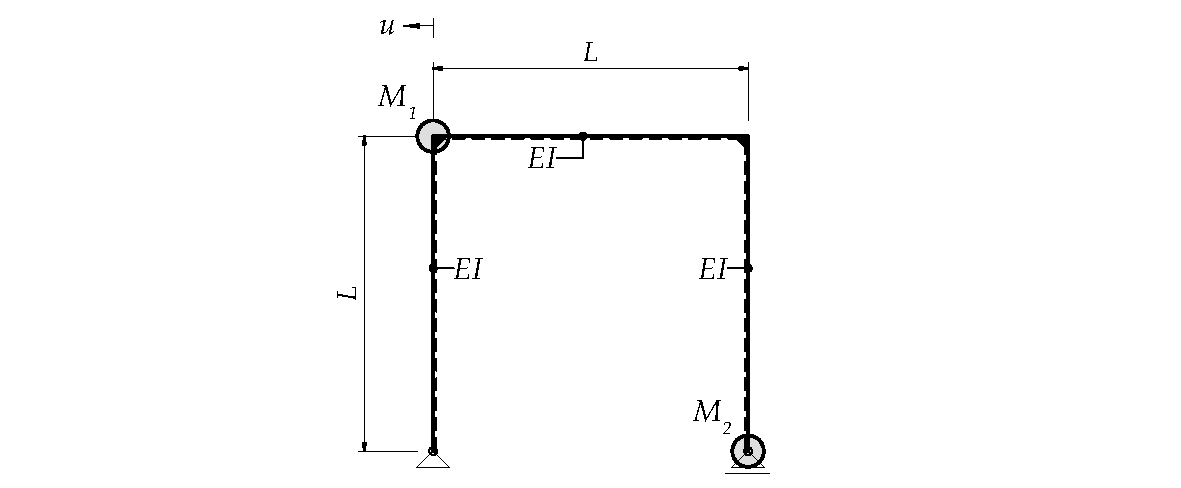
\includegraphics{index_files/mediabag/bilder/aufgabe_mms_nach_system.pdf}

}

\caption{\label{fig-mms_nach_system}Statisches System des
2-Massenschwingers}

\end{figure}

Gesucht:

\begin{itemize}
\item
  Eigenkreisfrequenz \(\omega\)
\item
  Eigenformen - Normierung auf \[\phi_1^T = 
  \begin{bmatrix}
  1 &  \\
  \end{bmatrix} \] \[\phi_2^T =
  \begin{bmatrix}
   & 1 \\
  \end{bmatrix}\]
\item
  Skizze der Eigenformen
\item
  Kontrolle der Orthogonalitätsbedingung
\end{itemize}

Gegeben:

\begin{itemize}
\tightlist
\item
  Dehnsteifigkeit aller Stäbe \(E\cdot A = \infty\)
\end{itemize}

\hypertarget{tbl-parameter_mms1}{}
\begin{longtable}[]{@{}
  >{\raggedright\arraybackslash}p{(\columnwidth - 2\tabcolsep) * \real{0.5000}}
  >{\raggedright\arraybackslash}p{(\columnwidth - 2\tabcolsep) * \real{0.5000}}@{}}
\caption{\label{tbl-parameter_mms1}Parameter der
Aufgabenstellung}\tabularnewline
\toprule\noalign{}
\endfirsthead
\endhead
\bottomrule\noalign{}
\endlastfoot
\(EI = 20000000000000 \text{mm}^{2} \text{N}\) & \(L = 4 \text{m}\) \\
\(m_{1} = \frac{1000 \text{N} \text{s}^{2}}{\text{m}}\) &
\(m_{2} = \frac{1000 \text{N} \text{s}^{2}}{\text{m}}\) \\
\end{longtable}

\newpage{}

\hypertarget{musterluxf6sung-8}{%
\section{Musterlösung}\label{musterluxf6sung-8}}

\hypertarget{sec-mms_nach_nachgiebigkeit}{%
\subsection{\texorpdfstring{Nachgiebigkeitsmatrix
\(\mathbf{D}\)}{Nachgiebigkeitsmatrix \textbackslash mathbf\{D\}}}\label{sec-mms_nach_nachgiebigkeit}}

Die Steifigkeitsmatrix lässt sich durch Invertierung der
Nachgiebigkeitsmatrix beschreiben. Die Nachgiebigkeitsmatrix
\(\mathbf{D}\) beschreibt die Deformation an einem Massenpunkt. Die
Einträge der \(\mathbf{D}\) - Matrix beschreiben die Deformationen für
unterschiedliche Laststellungen.

\begin{equation}\protect\hypertarget{eq-mms_nach_invert_K}{}{
\mathbf{K} = \mathbf{D^{-1}}
}\label{eq-mms_nach_invert_K}\end{equation}

\begin{figure}[H]

{\centering 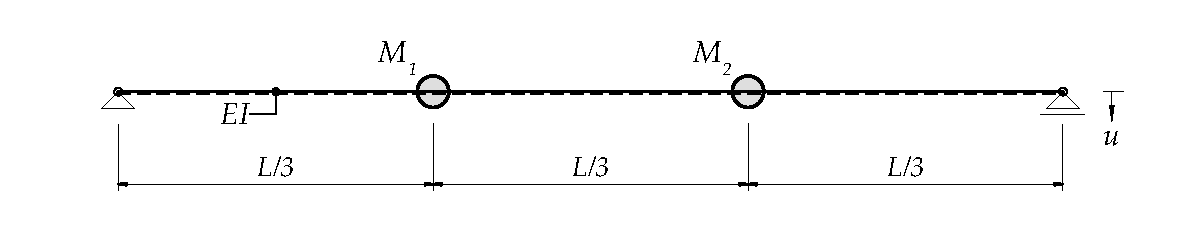
\includegraphics{index_files/mediabag/bilder/aufgabe_mms_nach_beispielbalken.pdf}

}

\caption{\label{fig-mms_nach_2mms}Balken mit 2 Einzelmassen}

\end{figure}

Für einen 2-Massenschwinger, wie in Abbildung~\ref{fig-mms_nach_2mms} ,
hat die Nachgiebigkeitsmatrix folgende Form:

\begin{equation}\protect\hypertarget{eq-mms_nach_nachgiebigkeitsmatrix}{}{
\mathbf{D} = \frac{1}{EI}\cdot \begin{bmatrix}
\delta_{11} & \delta_{12}\\
\delta_{21} & \delta_{22} 
\end{bmatrix}
}\label{eq-mms_nach_nachgiebigkeitsmatrix}\end{equation}

wobei gilt:

\(\delta_{ab}\) : \(a\) ist die Lastsituation, \(b\) ist die Masse.

\hypertarget{anwendung}{%
\subsubsection{Anwendung}\label{anwendung}}

\begin{figure}[H]

{\centering 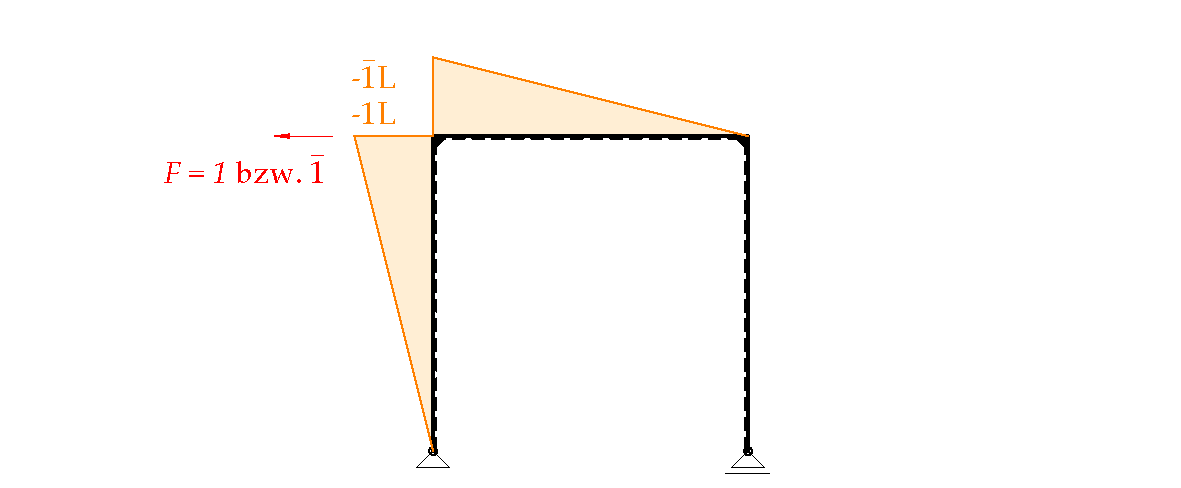
\includegraphics{index_files/mediabag/bilder/aufgabe_mms_nach_schnittgroessen1.pdf}

}

\caption{\label{fig-mms_nach_schnittgrössen1}Schnittgrössen für den
ersten Lastfall zur Bestimmung der Deformation}

\end{figure}

\begin{equation}\protect\hypertarget{eq-mms_nach_deformation}{}{
\delta_{ab} = \frac{1}{EI}\int_{0}^{L} M_a\bar{M_b} \,dx
}\label{eq-mms_nach_deformation}\end{equation}

Es werden 2 Laststellungen betrachtet, jeweils an einem Massenpunkt.
Dabei ist Beachtung der Einheit der Einwirkung zu schenken. Diese wird
einheitslos angesetzt.

\begin{figure}[H]

{\centering 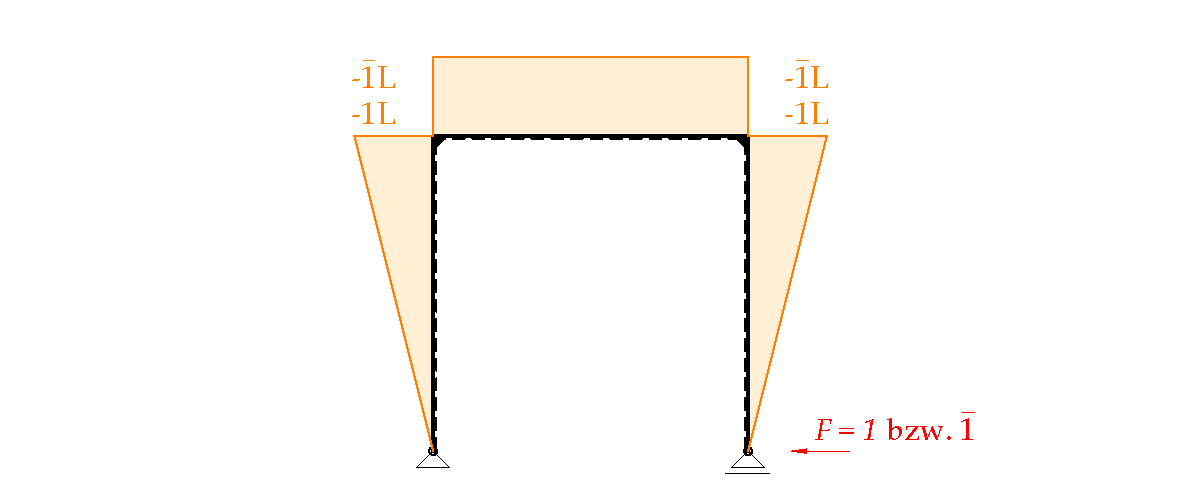
\includegraphics{index_files/mediabag/bilder/aufgabe_mms_nach_schnittgroessen2.pdf}

}

\caption{\label{fig-mms_nach_schnittgrössen2}Schnittgrössen für den
zweiten Lastfall zur Bestimmung der Deformation}

\end{figure}

\begin{equation}\delta_{11} = \frac{2 L^{3}}{3 EI}\end{equation}

\begin{equation}\delta_{12} = \frac{5 L^{3}}{6 EI}\end{equation}

\begin{equation}\delta_{21} = \frac{5 L^{3}}{6 EI}\end{equation}

\begin{equation}\delta_{22} = \frac{5 L^{3}}{3 EI}\end{equation}

\begin{equation}D = \left[\begin{matrix}\frac{2 L^{3}}{3 EI} & \frac{5 L^{3}}{6 EI}\\\frac{5 L^{3}}{6 EI} & \frac{5 L^{3}}{3 EI}\end{matrix}\right]\end{equation}

\begin{equation}K = \left[\begin{matrix}\frac{4 EI}{L^{3}} & - \frac{2 EI}{L^{3}}\\- \frac{2 EI}{L^{3}} & \frac{8 EI}{5 L^{3}}\end{matrix}\right]\end{equation}

\hypertarget{eigenvektoren-1}{%
\subsection{Eigenvektoren}\label{eigenvektoren-1}}

Die Bewegungsgleichung für einen ungedämpften, frei schwingenden
Mehrmassenschwinger lässt sich folgender massen aufstellen:

\begin{equation}\protect\hypertarget{eq-mms_nach_bewegungsgleichung}{}{
\mathbf{M u''(t) + K u(t)} = 0
}\label{eq-mms_nach_bewegungsgleichung}\end{equation}

Die Modale Analyse entkoppelt die Gleichungen um diese unabhängig von
einander zu lösen.

\hypertarget{massenmatrix-mathbfm-1}{%
\subsubsection{\texorpdfstring{Massenmatrix
\(\mathbf{M}\)}{Massenmatrix \textbackslash mathbf\{M\}}}\label{massenmatrix-mathbfm-1}}

\begin{equation}M = \left[\begin{matrix}m_{1} & 0\\0 & m_{2}\end{matrix}\right]\end{equation}

\hypertarget{eigenkreisfrequenzen-2}{%
\subsubsection{Eigenkreisfrequenzen}\label{eigenkreisfrequenzen-2}}

Bei einem Mehrmassenschwinger gibt es entsprechend den Freiheitsgraden
Eigenkreisfrequenzen \(\omega_n\). Diese lassen sich anhand
Gleichung~\ref{eq-mms_nach_eigenkreisfrequenzen} bestimmen:

\begin{equation}\protect\hypertarget{eq-mms_nach_eigenkreisfrequenzen}{}{
\det{[\mathbf{K}-\omega_n^2 \mathbf{M}]=0}
}\label{eq-mms_nach_eigenkreisfrequenzen}\end{equation}

\begin{equation}\omega_{1} = \frac{12.1}{\text{s}}\end{equation}

\begin{equation}\omega_{2} = \frac{40.0}{\text{s}}\end{equation}

\hypertarget{eigenvektoren-phi-1}{%
\subsubsection{\texorpdfstring{Eigenvektoren
\(\phi\)}{Eigenvektoren \textbackslash phi}}\label{eigenvektoren-phi-1}}

\begin{equation}\protect\hypertarget{eq-mms_nach_eigenvektor}{}{
\phi_n = \begin{bmatrix}
\phi_{1n}\\
\phi_{2n} 
\end{bmatrix}
}\label{eq-mms_nach_eigenvektor}\end{equation}

\begin{equation}\protect\hypertarget{eq-mms_nach_eigenvektor_bestimmung}{}{
[\mathbf{K}-\omega_n^2 \mathbf{M}]\cdot \begin{bmatrix}
\phi_{1n}\\
\phi_{2n} 
\end{bmatrix}
=0
}\label{eq-mms_nach_eigenvektor_bestimmung}\end{equation}

Dazu ist die entsprechende Normierung aus der Aufgabenstellung zu
berücksichtigen. Generell gilt, den Vektor auf den Maximalwert zu
normieren, bzw. diesen auf 1 zu setzen.

\begin{equation}\left[\begin{matrix}- \frac{2 EI \phi_{21}}{L^{3}} + \phi_{11} \cdot \left(\frac{4 EI}{L^{3}} - m_{1} \cdot \left(\frac{4 EI}{5 L^{3} m_{2}} + \frac{2 EI}{L^{3} m_{1}} - \frac{2 EI \sqrt{4 m_{1}^{2} + 5 m_{1} m_{2} + 25 m_{2}^{2}}}{5 L^{3} m_{1} m_{2}}\right)\right)\\- \frac{2 EI \phi_{11}}{L^{3}} + \phi_{21} \cdot \left(\frac{8 EI}{5 L^{3}} - m_{2} \cdot \left(\frac{4 EI}{5 L^{3} m_{2}} + \frac{2 EI}{L^{3} m_{1}} - \frac{2 EI \sqrt{4 m_{1}^{2} + 5 m_{1} m_{2} + 25 m_{2}^{2}}}{5 L^{3} m_{1} m_{2}}\right)\right)\end{matrix}\right] = \left[\begin{matrix}0\\0\end{matrix}\right]\end{equation}

\begin{equation}\phi_{1} = \left[\begin{matrix}0.566\\1.0\end{matrix}\right]\end{equation}

\begin{equation}\left[\begin{matrix}- \frac{2 EI \phi_{22}}{L^{3}} + \phi_{12} \cdot \left(\frac{4 EI}{L^{3}} - m_{1} \cdot \left(\frac{4 EI}{5 L^{3} m_{2}} + \frac{2 EI}{L^{3} m_{1}} + \frac{2 EI \sqrt{4 m_{1}^{2} + 5 m_{1} m_{2} + 25 m_{2}^{2}}}{5 L^{3} m_{1} m_{2}}\right)\right)\\- \frac{2 EI \phi_{12}}{L^{3}} + \phi_{22} \cdot \left(\frac{8 EI}{5 L^{3}} - m_{2} \cdot \left(\frac{4 EI}{5 L^{3} m_{2}} + \frac{2 EI}{L^{3} m_{1}} + \frac{2 EI \sqrt{4 m_{1}^{2} + 5 m_{1} m_{2} + 25 m_{2}^{2}}}{5 L^{3} m_{1} m_{2}}\right)\right)\end{matrix}\right] = \left[\begin{matrix}0\\0\end{matrix}\right]\end{equation}

\begin{equation}\phi_{2} = \left[\begin{matrix}1.0\\-0.566\end{matrix}\right]\end{equation}

\hypertarget{sec-mms_nach_ortho}{%
\subsubsection{Orthogonalitätsbedingung}\label{sec-mms_nach_ortho}}

Um eine modale Analyse des Systems durchzuführen, gilt es die
Orthogonalität der Eigenvektoren zu gewährleisten. Die Modale Analyse
wird in folgenden Beispielen ,wie in Kapitel~\ref{sec-tilger},
angewendet.

Dies gilt es für die Massenmatrix zu kontrollieren:

\begin{equation}\phi_{1}^{T} M \phi_{1} = \left[\begin{matrix}\frac{1.32 \cdot 10^{3} \text{N} \text{s}^{2}}{\text{m}}\end{matrix}\right]\end{equation}

\begin{equation}\phi_{2}^{T} M \phi_{2} = \left[\begin{matrix}\frac{1.32 \cdot 10^{3} \text{N} \text{s}^{2}}{\text{m}}\end{matrix}\right]\end{equation}

\begin{equation}\phi_{2}^{T} M \phi_{1} = \left[\begin{matrix}0\end{matrix}\right]\end{equation}

\begin{equation}\phi_{1}^{T} M \phi_{2} = \left[\begin{matrix}0\end{matrix}\right]\end{equation}

Sowohl auch für die Steifigkeitsmatrix:

\begin{equation}\phi_{1}^{T} K \phi_{1} = \left[\begin{matrix}\frac{1.93 \cdot 10^{5} \text{N}}{\text{m}}\end{matrix}\right]\end{equation}

\begin{equation}\phi_{2}^{T} K \phi_{2} = \left[\begin{matrix}\frac{2.12 \cdot 10^{6} \text{N}}{\text{m}}\end{matrix}\right]\end{equation}

\begin{equation}\phi_{2}^{T} K \phi_{1} = \left[\begin{matrix}0\end{matrix}\right]\end{equation}

\begin{equation}\phi_{1}^{T} K \phi_{2} = \left[\begin{matrix}0\end{matrix}\right]\end{equation}

Die Orthogonalitätsbedingung ist erfüllt!

Zur effektiven Entkoppelung der Gleichungen muss die
Orthogonalitätsbedingung eingehalten sein. Durch die Orthogonalität der
Vektoren \(\phi_1\) und \(\phi_2\) kann mittels einem
Einmassenschwingers sämtliches Verhalten von \(\phi_1\) beschrieben
werden und mittels einem zweiten Einmassenschwinger sämtliches Verhalten
von \(\phi_2\). Ist die Orthogonalität nicht gegeben, so müsste der
erste Einmassenschwinger Anteile aus \(\phi_1\) und \(\phi_2\)
beschreiben.

\begin{figure}

\begin{minipage}[t]{0.50\linewidth}

{\centering 

\raisebox{-\height}{

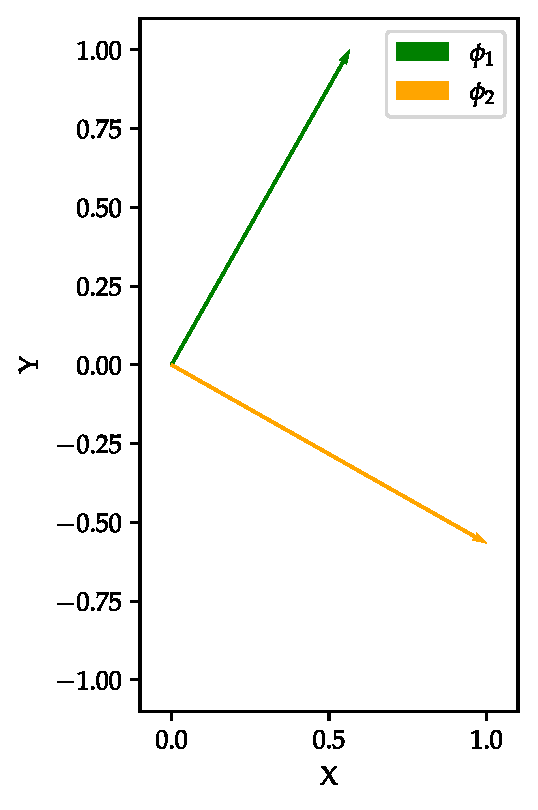
\includegraphics{index_files/mediabag/mms_01_files/figure-pdf/fig-ems_nach_ortho-output-1.pdf}

}

}

\subcaption{\label{fig-ems_nach_ortho-1}Erfüllte
Orthogonalitätsbedingung}
\end{minipage}%
%
\begin{minipage}[t]{0.50\linewidth}

{\centering 

\raisebox{-\height}{

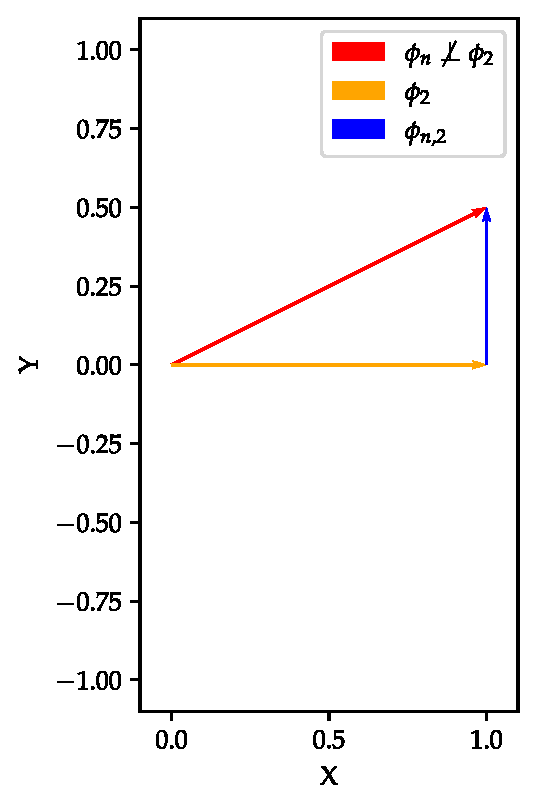
\includegraphics{index_files/mediabag/mms_01_files/figure-pdf/fig-ems_nach_ortho-output-2.pdf}

}

}

\subcaption{\label{fig-ems_nach_ortho-2}Nicht erfüllte
Orthogonalitätsbedingung}
\end{minipage}%

\caption{\label{fig-ems_nach_ortho}Visualisierung des Einflusses der
Orthogonalität der Eigenvektoren}

\end{figure}

Wie in Abbildung~\ref{fig-ems_nach_ortho} dargestellt, wird der rote
Vektor \(\phi_n\) durch den orangenen Vektor \(\phi_2\) beschrieben,
sowie durch seine \(Y\) Komponente \(\phi_{n,2}\). Folglich steht
\(\phi_n\) nicht orthogonal auf \(\phi_2\) und lässt sich nicht ohne
\(\phi_2\) beschreiben. Die Entkoppelung ist nicht möglich.

Nebenbei, dies lässt sich für einen zweidimensionalen Fall, sprich
Zweimassenschwinger darstellen. Das Verfahren kann auf beliebig viele
Dimensionen erweitert werden, die Darstellung dieser ist jedoch nicht
mehr möglich.

\hypertarget{eigenformen-1}{%
\subsection{Eigenformen}\label{eigenformen-1}}

\begin{figure}[H]

{\centering 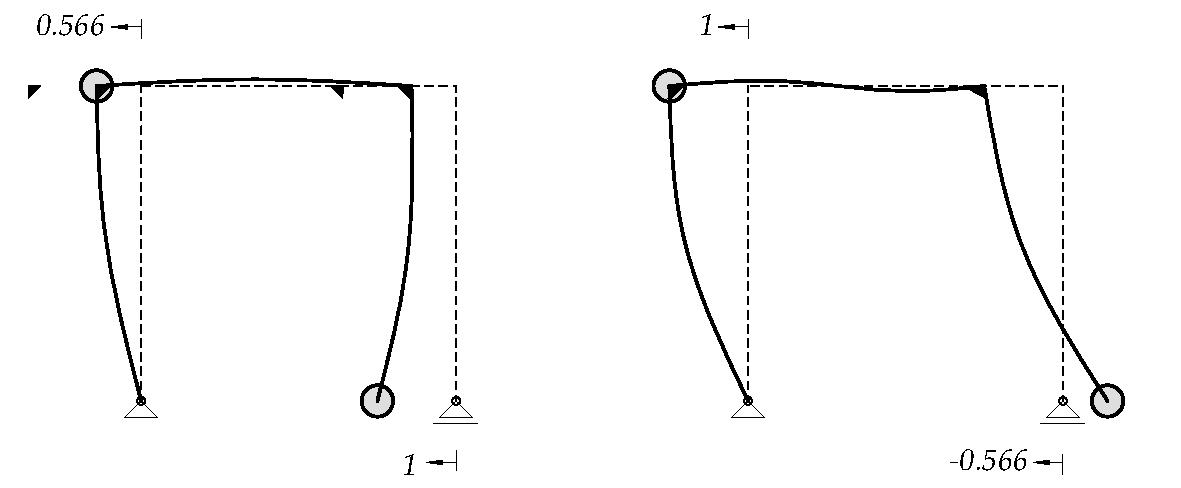
\includegraphics{index_files/mediabag/bilder/aufgabe_mms_nach_eigenvekt1.pdf}

}

\caption{\label{fig-mms_nach_eigenformen}Die beiden Eigenform skizziert}

\end{figure}

\hypertarget{sec-tilger}{%
\chapter{Beispiel: Balken mit Tilger}\label{sec-tilger}}

\hypertarget{aufgabenstellung-12}{%
\section{Aufgabenstellung}\label{aufgabenstellung-12}}

Das Beispiel ist die Weiterführung der Aufgabe in
Kapitel~\ref{sec-ems_untilg}. Ein einfacher Balken mit einer
Einzelmasse, welcher in dieser Aufgabe mit Tilger ausgestattet ist, ist
in Abbildung~\ref{fig-mms_tilg_tilger} dargestellt. Die Masse erfährt
eine dynamische Einwirkung durch die Funktion \(F(t)\).

\begin{figure}[H]

{\centering 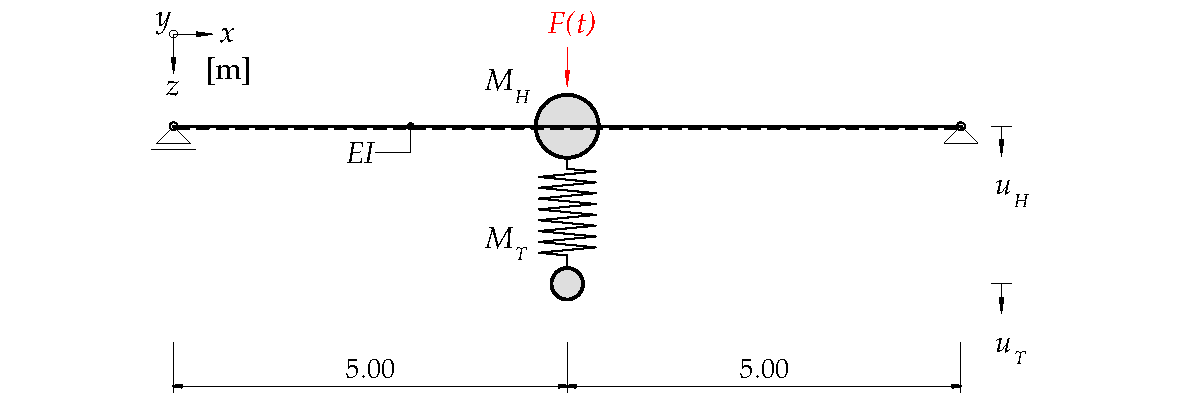
\includegraphics{index_files/mediabag/bilder/aufgabe_mms_tilg_system.pdf}

}

\caption{\label{fig-mms_tilg_tilger}Statisches System des Balkens mit
Tilger}

\end{figure}

Gesucht:

\begin{itemize}
\tightlist
\item
  Normierte Eigenform
\item
  Maximale dynamische Verformung mittels stationärer Lösung
\item
  Maximale dynamische Beschleunigung mittels stationärer Lösung
\end{itemize}

Gegeben:

\hypertarget{tbl-parameter_mms4}{}
\begin{longtable}[]{@{}
  >{\raggedright\arraybackslash}p{(\columnwidth - 2\tabcolsep) * \real{0.5000}}
  >{\raggedright\arraybackslash}p{(\columnwidth - 2\tabcolsep) * \real{0.5000}}@{}}
\caption{\label{tbl-parameter_mms4}Parameter der
Aufgabenstellung}\tabularnewline
\toprule\noalign{}
\endfirsthead
\endhead
\bottomrule\noalign{}
\endlastfoot
\(E = \frac{200000 \text{N}}{\text{mm}^{2}}\) &
\(F_{0} = 800.0 \text{N}\) \\
\(I = 200000000 \text{mm}^{4}\) & \(L = 5 \text{m}\) \\
\(k_{T} = \frac{90000 \text{N}}{\text{m}}\) &
\(m_{H} = \frac{2000 \text{N} \text{s}^{2}}{\text{m}}\) \\
\(m_{T} = \frac{150 \text{N} \text{s}^{2}}{\text{m}}\) &
\(\omega = \frac{12.6}{\text{s}}\) \\
\(\phi_{11} = 1\) & \(\phi_{12} = 1\) \\
\(\zeta = 0.0\) & \\
\end{longtable}

\[
F(t) = F_0 \cdot \sin(\omega\cdot t) = 0.8 \text{kN} \cdot (12.6 \frac{\text{rad}}{\text{s}}\cdot t)
\]

\newpage{}

\hypertarget{musterluxf6sung-9}{%
\section{Musterlösung}\label{musterluxf6sung-9}}

\hypertarget{bemerkung-tilgerauslegung}{%
\subsection{Bemerkung Tilgerauslegung}\label{bemerkung-tilgerauslegung}}

Die Auslegung des Tilgers kann folgender massen geschehen:

\begin{itemize}
\tightlist
\item
  Tilgermasse \(5\%\) von der Masse des Hauptträgers.
\item
  Optimale Frequenz bestimmen:
  \begin{equation}\protect\hypertarget{eq-mms_tilg_optimale_frequenz}{}{
  f_{T,opt} =\frac{f_H}{1+\frac{m_T}{m_H}}
  }\label{eq-mms_tilg_optimale_frequenz}\end{equation}
\item
  Daraus die optimale Steifigkeit bestimmen:
  \begin{equation}\protect\hypertarget{eq-mms_tilg_optimale_steif}{}{
  k_{T,opt} = (2 \pi f_{T,opt})^2
  }\label{eq-mms_tilg_optimale_steif}\end{equation}
\end{itemize}

\hypertarget{steifigkeitsmatrix-mathbfk}{%
\subsection{\texorpdfstring{Steifigkeitsmatrix
\(\mathbf{K}\)}{Steifigkeitsmatrix \textbackslash mathbf\{K\}}}\label{steifigkeitsmatrix-mathbfk}}

\begin{figure}[H]

{\centering 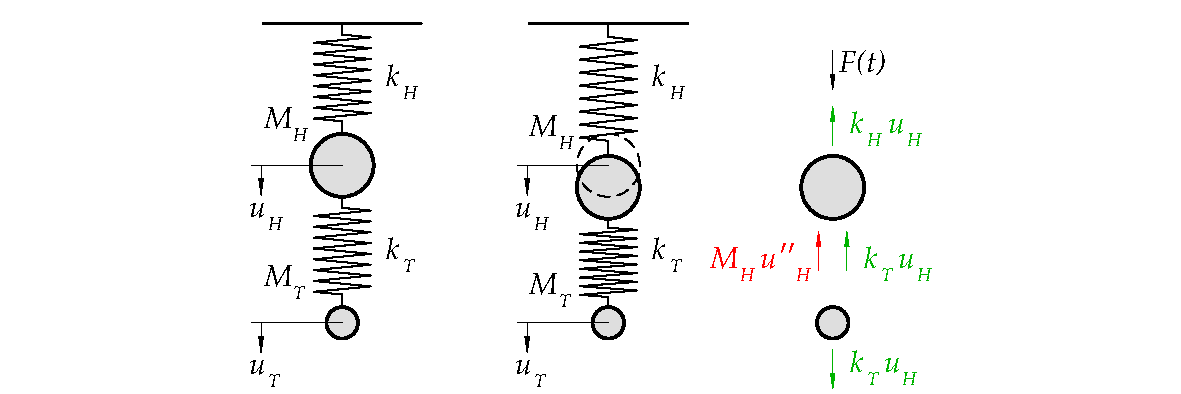
\includegraphics{index_files/mediabag/bilder/aufgabe_mms_tilg_auslenk2.pdf}

}

\caption{\label{fig-mms_tilg_auslenkung_1}Verformungen am ersten
Freiheitsgrad}

\end{figure}

Wichtig dabei sind die Richtungen der Kräfte. Als Denkstütze gilt
folgendes:

\begin{itemize}
\tightlist
\item
  Der Auslenkung um \(u\) wirkt die Federkraft entgegen, welche \(k u\)
  entspricht.
\item
  Zusätzlich wirkt die Trägheitskraft der Auslenkung entgegen, welche
  \(m u''\) entspricht.
\item
  Nach der Betrachtung des ausgelenkten Punkts, kann mittels
  \emph{Actio-Reactio}-Prinzip das ``\emph{Stockwerk}'' ins
  Gleichgewicht gebracht werden.
\item
  Vorzeichen sind gegen der Bewegungsrichtig positiv.
\end{itemize}

\begin{figure}[H]

{\centering 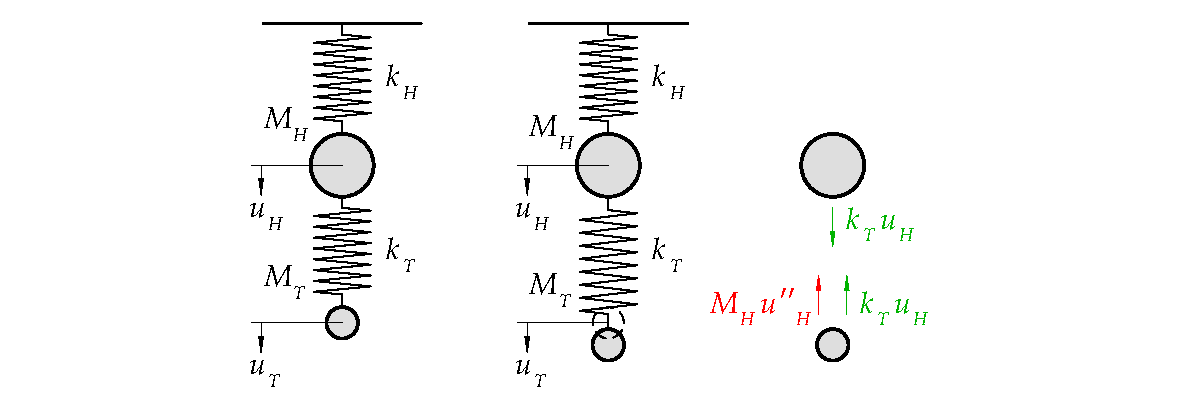
\includegraphics{index_files/mediabag/bilder/aufgabe_mms_tilg_auslenk1.pdf}

}

\caption{\label{fig-mms_tilg_auslenkung_2}Verformungen am zweiten
Freiheitsgrad}

\end{figure}

\begin{equation}K = \left[\begin{matrix}k_{H} + k_{T} & - k_{T}\\- k_{T} & k_{T}\end{matrix}\right]\end{equation}

\begin{equation}K = \left[\begin{matrix}\frac{2010000 \text{N}}{\text{m}} & - \frac{90000 \text{N}}{\text{m}}\\- \frac{90000 \text{N}}{\text{m}} & \frac{90000 \text{N}}{\text{m}}\end{matrix}\right]\end{equation}

\hypertarget{eigenvektoren-2}{%
\subsection{Eigenvektoren}\label{eigenvektoren-2}}

\hypertarget{massenmatrix-mathbfm-2}{%
\subsubsection{\texorpdfstring{Massenmatrix
\(\mathbf{M}\)}{Massenmatrix \textbackslash mathbf\{M\}}}\label{massenmatrix-mathbfm-2}}

Die Massenmatrix folgt dem gleichen Aufbau der Steifigkeitsmatrix. Es
gelten die gleichen Vorzeichenregelungen. Die Einträge beziehen sich auf
Abbildung~\ref{fig-mms_tilg_auslenkung_2} und
Abbildung~\ref{fig-mms_tilg_auslenkung_1}.

\begin{equation}M = \left[\begin{matrix}m_{H} & 0\\0 & m_{T}\end{matrix}\right]\end{equation}

\begin{equation}M = \left[\begin{matrix}\frac{2000 \text{N} \text{s}^{2}}{\text{m}} & 0\\0 & \frac{150 \text{N} \text{s}^{2}}{\text{m}}\end{matrix}\right]\end{equation}

\hypertarget{eigenkreisfrequenzen-3}{%
\subsubsection{Eigenkreisfrequenzen}\label{eigenkreisfrequenzen-3}}

Bei einem Mehrmassenschwinger gibt es entsprechend den Freiheitsgraden
Eigenkreisfrequenzen \(\omega_n\). Diese lassen sich anhand folgender
Gleichung bestimmen:

\begin{equation}\protect\hypertarget{eq-mms_tilg_eigenkreisfrequenzen}{}{
\det{[\mathbf{K}-\omega_n^2 \mathbf{M}]=0}
}\label{eq-mms_tilg_eigenkreisfrequenzen}\end{equation}

\begin{equation}\omega_{1} = \frac{23.3}{\text{s}}\end{equation}

\begin{equation}\omega_{2} = \frac{32.6}{\text{s}}\end{equation}

\hypertarget{eigenvektoren-mathbfphi}{%
\subsubsection{\texorpdfstring{Eigenvektoren
\(\mathbf{\phi}\)}{Eigenvektoren \textbackslash mathbf\{\textbackslash phi\}}}\label{eigenvektoren-mathbfphi}}

\begin{equation}\protect\hypertarget{eq-mms_tilg_eigenvek}{}{
\phi_n = \begin{bmatrix}
\phi_{1n}\\
\phi_{2n} 
\end{bmatrix}
}\label{eq-mms_tilg_eigenvek}\end{equation}
\begin{equation}\protect\hypertarget{eq-mms_tilg_eigenvek_eq}{}{
[\mathbf{K}-\omega_n^2 \mathbf{M}]\cdot \begin{bmatrix}
\phi_{1n}\\
\phi_{2n} 
\end{bmatrix}
=0}\label{eq-mms_tilg_eigenvek_eq}\end{equation}

Dazu ist die entsprechende Normierung aus der Aufgabenstellung zu
berücksichtigen.

\begin{equation}\left[\begin{matrix}\frac{- k_{T} m_{T} \phi_{21} + \frac{\phi_{11} \left(- k_{T} m_{H} + m_{T} \left(k_{H} + k_{T}\right) + \sqrt{k_{H}^{2} m_{T}^{2} - 2 k_{H} k_{T} m_{H} m_{T} + 2 k_{H} k_{T} m_{T}^{2} + k_{T}^{2} m_{H}^{2} + 2 k_{T}^{2} m_{H} m_{T} + k_{T}^{2} m_{T}^{2}}\right)}{2}}{m_{T}}\\\frac{- k_{T} m_{H} \phi_{11} + \frac{\phi_{21} \left(k_{T} m_{H} - m_{T} \left(k_{H} + k_{T}\right) + \sqrt{k_{H}^{2} m_{T}^{2} - 2 k_{H} k_{T} m_{H} m_{T} + 2 k_{H} k_{T} m_{T}^{2} + k_{T}^{2} m_{H}^{2} + 2 k_{T}^{2} m_{H} m_{T} + k_{T}^{2} m_{T}^{2}}\right)}{2}}{m_{H}}\end{matrix}\right] = \left[\begin{matrix}0\\0\end{matrix}\right]\end{equation}

\begin{equation}\phi_{1} = \left[\begin{matrix}1.0\\10.3\end{matrix}\right]\end{equation}

\begin{equation}\left[\begin{matrix}\frac{- k_{T} m_{T} \phi_{22} + \frac{\phi_{12} \left(- k_{T} m_{H} + m_{T} \left(k_{H} + k_{T}\right) - \sqrt{k_{H}^{2} m_{T}^{2} - 2 k_{H} k_{T} m_{H} m_{T} + 2 k_{H} k_{T} m_{T}^{2} + k_{T}^{2} m_{H}^{2} + 2 k_{T}^{2} m_{H} m_{T} + k_{T}^{2} m_{T}^{2}}\right)}{2}}{m_{T}}\\\frac{- k_{T} m_{H} \phi_{12} + \frac{\phi_{22} \left(k_{T} m_{H} - m_{T} \left(k_{H} + k_{T}\right) - \sqrt{k_{H}^{2} m_{T}^{2} - 2 k_{H} k_{T} m_{H} m_{T} + 2 k_{H} k_{T} m_{T}^{2} + k_{T}^{2} m_{H}^{2} + 2 k_{T}^{2} m_{H} m_{T} + k_{T}^{2} m_{T}^{2}}\right)}{2}}{m_{H}}\end{matrix}\right] = \left[\begin{matrix}0\\0\end{matrix}\right]\end{equation}

\begin{equation}\phi_{2} = \left[\begin{matrix}1.0\\-1.3\end{matrix}\right]\end{equation}

\hypertarget{orthogonalituxe4tsbedingung-1}{%
\subsubsection{Orthogonalitätsbedingung}\label{orthogonalituxe4tsbedingung-1}}

Zur Entkoppelung des Systems wird die Orthogonalität der Eigenvektoren
kontrolliert. Siehe Kapitel~\ref{sec-mms_nach_ortho} für eine
ausführliche Erklärung.

\begin{equation}\phi_{1}^{T} M \phi_{1} = \left[\begin{matrix}\frac{1.79 \cdot 10^{4} \text{N} \text{s}^{2}}{\text{m}}\end{matrix}\right]\end{equation}

\begin{equation}\phi_{2}^{T} M \phi_{2} = \left[\begin{matrix}\frac{2.25 \cdot 10^{3} \text{N} \text{s}^{2}}{\text{m}}\end{matrix}\right]\end{equation}

\begin{equation}\phi_{2}^{T} M \phi_{1} = \left[\begin{matrix}\frac{6.103516 \cdot 10^{-5} \text{N} \text{s}^{2}}{\text{m}}\end{matrix}\right]\end{equation}

\begin{equation}\phi_{1}^{T} M \phi_{2} = \left[\begin{matrix}\frac{6.103516 \cdot 10^{-5} \text{N} \text{s}^{2}}{\text{m}}\end{matrix}\right]\end{equation}

Es ist eine kleine numerische Differenz zu erkennen welche nicht
relevant sind.

\begin{equation}\phi_{1}^{T} K \phi_{1} = \left[\begin{matrix}\frac{9.7 \cdot 10^{6} \text{N}}{\text{m}}\end{matrix}\right]\end{equation}

\begin{equation}\phi_{2}^{T} K \phi_{2} = \left[\begin{matrix}\frac{2.39 \cdot 10^{6} \text{N}}{\text{m}}\end{matrix}\right]\end{equation}

\begin{equation}\phi_{2}^{T} K \phi_{1} = \left[\begin{matrix}0\end{matrix}\right]\end{equation}

\begin{equation}\phi_{1}^{T} K \phi_{2} = \left[\begin{matrix}0\end{matrix}\right]\end{equation}

\hypertarget{modale-analyse}{%
\subsection{Modale Analyse}\label{modale-analyse}}

Die Bewegungsgleichung für einen ungedämpften, periodisch, harmonisch
angeregten Mehrmassenschwinger lässt sich folgend beschreiben:

\begin{equation}\protect\hypertarget{eq-mms_tilg_bewegungsgleichung_nohomo}{}{
\mathbf{M u''(t) + K u = F(t)}
}\label{eq-mms_tilg_bewegungsgleichung_nohomo}\end{equation}

Die Matrix-Gleichung beschreibt ein System aus Differentialgleichungen.
Die Modale Analyse zielt darauf ab, diese zu entkoppeln. Bezogen auf den
Mehrmassenschwinger heisst eine Entkoppelung, dass diese in
Einmassenschwinger aufgeteilt werden. Dies wird nun schrittweise
durchgeführt.

\hypertarget{modal--und-spektralmatrix}{%
\subsubsection{Modal- und
Spektralmatrix}\label{modal--und-spektralmatrix}}

Mittels der Modal- und Spektralmatrix können die generalisierten Grössen
ermittelt werden. Diese sind die eigenschaften der einzelnen
Einmassenschwinger. Die generalisierten Werte besitzen keine
physikalischen Bedeutung, sie sind abhängig von der Wahl der
Eigenvektoren, welche bekanntlich von der Normierung abhängen.

Anhand der Bewegungsgleichung können die generalisierten Grössen
bestimmt werden, es gilt:

\[\Phi^T M \Phi u''(t) + \Phi^T K \Phi u(t) = \Phi^T F(t)\]

\[M^*u''(t) + K^* u(t) = F^* (t)\]

Alle \(N\)-Eigenwerte und alle \(N\)-Eigenvektoren können kompakt mit
Matrizen ausgedrückt werden:

\begin{equation}Modalmatrix = \Phi\end{equation}

\begin{equation}\Phi = \left[\begin{matrix}1.0 & 1.0\\10.3 & -1.295\end{matrix}\right]\end{equation}

\begin{equation}Spektralmatrix = \Omega^{2}\end{equation}

\begin{equation}\Omega^{2} = \left[\begin{matrix}\frac{541.7}{\text{s}^{2}} & 0\\0 & \frac{1063.0}{\text{s}^{2}}\end{matrix}\right]\end{equation}

\hypertarget{generalisierte-gruxf6ssen}{%
\subsubsection{Generalisierte Grössen}\label{generalisierte-gruxf6ssen}}

\begin{equation}M^{\star} = \left[\begin{matrix}\frac{17898.0 \text{N} \text{s}^{2}}{\text{m}} & 0\\0 & \frac{2251.6 \text{N} \text{s}^{2}}{\text{m}}\end{matrix}\right]\end{equation}

\begin{equation}K^{\star} = \left[\begin{matrix}\frac{9.6959 \cdot 10^{6} \text{N}}{\text{m}} & 0\\0 & \frac{2.3941 \cdot 10^{6} \text{N}}{\text{m}}\end{matrix}\right]\end{equation}

\begin{equation}F(t) = \left[\begin{matrix}800.0 \sin{\left(\frac{12.6 t}{\text{s}} \right)} \text{N}\\0\end{matrix}\right]\end{equation}

\begin{equation}F(t)^{\star} = \left[\begin{matrix}800.0 \sin{\left(\frac{12.6 t}{\text{s}} \right)} \text{N}\\800.0 \sin{\left(\frac{12.6 t}{\text{s}} \right)} \text{N}\end{matrix}\right]\end{equation}

\hypertarget{kontrolle-der-modalen-transformation}{%
\subsubsection{Kontrolle der modalen
Transformation}\label{kontrolle-der-modalen-transformation}}

\begin{equation}\omega_{1} = \frac{23.3}{\text{s}}\end{equation}

\begin{equation}\omega_{1 modal} = \frac{23.3}{\text{s}}\end{equation}

\begin{equation}\omega_{2} = \frac{32.61}{\text{s}}\end{equation}

\begin{equation}\omega_{2 modal} = \frac{32.61}{\text{s}}\end{equation}

\hypertarget{modale-huxf6hen}{%
\subsubsection{Modale Höhen}\label{modale-huxf6hen}}

Die modalen Höhen bestimmen sich aus
Gleichung~\ref{eq-mms_tilg_modale_hoehe}:

\begin{equation}\protect\hypertarget{eq-mms_tilg_modale_hoehe}{}{
H_n = \frac{L_n^\theta}{L_n}
}\label{eq-mms_tilg_modale_hoehe}\end{equation}

\begin{equation}\protect\hypertarget{eq-mms_tilg_L_n}{}{
L_n = \phi_n^T \cdot \mathbf{M 1}
}\label{eq-mms_tilg_L_n}\end{equation}

\begin{equation}\protect\hypertarget{eq-mms_tilg_L_n_theta}{}{
L_n^\theta = \sum_{j=1}^N H_j \cdot m_j \cdot \phi_{jn}
}\label{eq-mms_tilg_L_n_theta}\end{equation}

\ul{Wie sind modale Höhen mit diesem Beispiel zu bestimmen?}

\hypertarget{stationuxe4re-antwort-2}{%
\subsection{Stationäre Antwort}\label{stationuxe4re-antwort-2}}

Die stationäre Antwort wird mittels des Vergrösserungsfaktors bestimmt.

Die entkoppelte Differentialgleichung ist nun die folgende:

\begin{equation}\protect\hypertarget{eq-mms_tilger_erste_bewegungsgleichung}{}{
m^\star_1 q_1''(t) + k^\star_1 q_1(t) = F^\star_1(t) = F^\star_1 \sin(\omega t)
}\label{eq-mms_tilger_erste_bewegungsgleichung}\end{equation}

\begin{equation}\protect\hypertarget{eq-mms_tilger_zweite_bewegungsgleichung}{}{
m^\star_2 q_2''(t) + k^\star_2 q_2(t) = F^\star_2(t) = F^\star_2 \sin(\omega t)
}\label{eq-mms_tilger_zweite_bewegungsgleichung}\end{equation}

Lösen lässt sich dies mit dem bekannten Ansatz:

\begin{equation}\protect\hypertarget{eq-mms_tilger_ansatzfunktion}{}{
q_n(t) = A_n \sin(\omega t) + B_n \cos(\omega)
}\label{eq-mms_tilger_ansatzfunktion}\end{equation}

Hier wird jedoch mit dem Vorgehen des Vergrösserungsfaktors verfahren:

\hypertarget{verformung}{%
\subsubsection{Verformung}\label{verformung}}

\begin{equation}V_{1}{\left(\omega \right)} = \frac{1}{\sqrt{\frac{4 \omega^{2} \zeta_{}^{2}}{\omega_{1}^{2}} + \left(- \frac{\omega^{2}}{\omega_{1}^{2}} + 1\right)^{2}}}\end{equation}

\begin{equation}V_{1}{\left(\omega \right)} = 1.41\end{equation}

\begin{equation}q_{1 stat} = 0.0825 \text{mm}\end{equation}

\begin{equation}q_{1 max} = q_{1 stat} V_{1}{\left(\omega \right)}\end{equation}

\begin{equation}q_{1 max} = 0.117 \text{mm}\end{equation}

\begin{equation}V_{2}{\left(\omega \right)} = \frac{1}{\sqrt{\frac{4 \omega^{2} \zeta_{}^{2}}{\omega_{2}^{2}} + \left(- \frac{\omega^{2}}{\omega_{2}^{2}} + 1\right)^{2}}}\end{equation}

\begin{equation}V_{2}{\left(\omega \right)} = 1.18\end{equation}

\begin{equation}q_{2 stat} = 0.334 \text{mm}\end{equation}

\begin{equation}q_{2 max} = q_{2 stat} V_{2}{\left(\omega \right)}\end{equation}

\begin{equation}q_{2 max} = 0.393 \text{mm}\end{equation}

\hypertarget{effektive-deformation}{%
\paragraph{Effektive Deformation}\label{effektive-deformation}}

Die effektiven Grössen resultieren durch Multiplikation mit dem
Eigenvektor. Für die erste Eigenkreisfrequenz:

\begin{equation}u_{1 stat} = \phi_{1} q_{1 max}\end{equation}

\begin{equation}\left[\begin{matrix}u_{11stat}\\u_{21stat}\end{matrix}\right] = \left[\begin{matrix}0.117 \text{mm}\\1.2 \text{mm}\end{matrix}\right]\end{equation}

Sowie für die zweite Eigenkreisfrequenz:

\begin{equation}u_{2 stat} = \phi_{2} q_{2 max}\end{equation}

\begin{equation}\left[\begin{matrix}u_{12stat}\\u_{22stat}\end{matrix}\right] = \left[\begin{matrix}0.393 \text{mm}\\- 0.509 \text{mm}\end{matrix}\right]\end{equation}

Durch Addition der beiden Verformungen: \ul{Sollte hier die SRSS-Regel
verwendet werden?}

\begin{equation}u_{stat} = u_{1 stat} + u_{2 stat}\end{equation}

\begin{equation}\left[\begin{matrix}u_{1max}\\u_{2max}\end{matrix}\right] = \left[\begin{matrix}0.51 \text{mm}\\0.693 \text{mm}\end{matrix}\right]\end{equation}

\hypertarget{beschleunigung}{%
\subsubsection{Beschleunigung}\label{beschleunigung}}

\begin{equation}V_{a1 \omega} = \frac{V_{1 \omega} \omega^{2}}{\omega_{1}^{2}}\end{equation}

\begin{equation}V_{a1}{\left(\omega \right)} = 0.415\end{equation}

\begin{equation}\frac{d^{2}}{d t^{2}} q_{max} = \frac{0.0185 \text{m}}{\text{s}^{2}}\end{equation}

\begin{equation}V_{a2}{\left(\omega \right)} = 0.176\end{equation}

\begin{equation}\frac{d^{2}}{d t^{2}} q_{max} = \frac{0.0624 \text{m}}{\text{s}^{2}}\end{equation}

\hypertarget{effektive-beschleunigung}{%
\paragraph{Effektive Beschleunigung}\label{effektive-beschleunigung}}

Gleiches Vorgehen wie bei der Deformation.

\begin{equation}\left[\begin{matrix}\frac{d^{2}}{d t^{2}} u_{1max}\\\frac{d^{2}}{d t^{2}} u_{2max}\end{matrix}\right] = \left[\begin{matrix}\frac{0.0809 \text{m}}{\text{s}^{2}}\\\frac{0.11 \text{m}}{\text{s}^{2}}\end{matrix}\right]\end{equation}

\hypertarget{beispiel-antwortspektrenverfahren-an-einem-dreistuxf6ckigen-gebuxe4ude}{%
\chapter{Beispiel: Antwortspektrenverfahren an einem dreistöckigen
Gebäude}\label{beispiel-antwortspektrenverfahren-an-einem-dreistuxf6ckigen-gebuxe4ude}}

Das System in Abbildung~\ref{fig-mms_3er_system} zeigt eine
dreistöckiges Gebäude. Modelliert wird dies als Dreimassenschwinger.

\begin{figure}[H]

{\centering 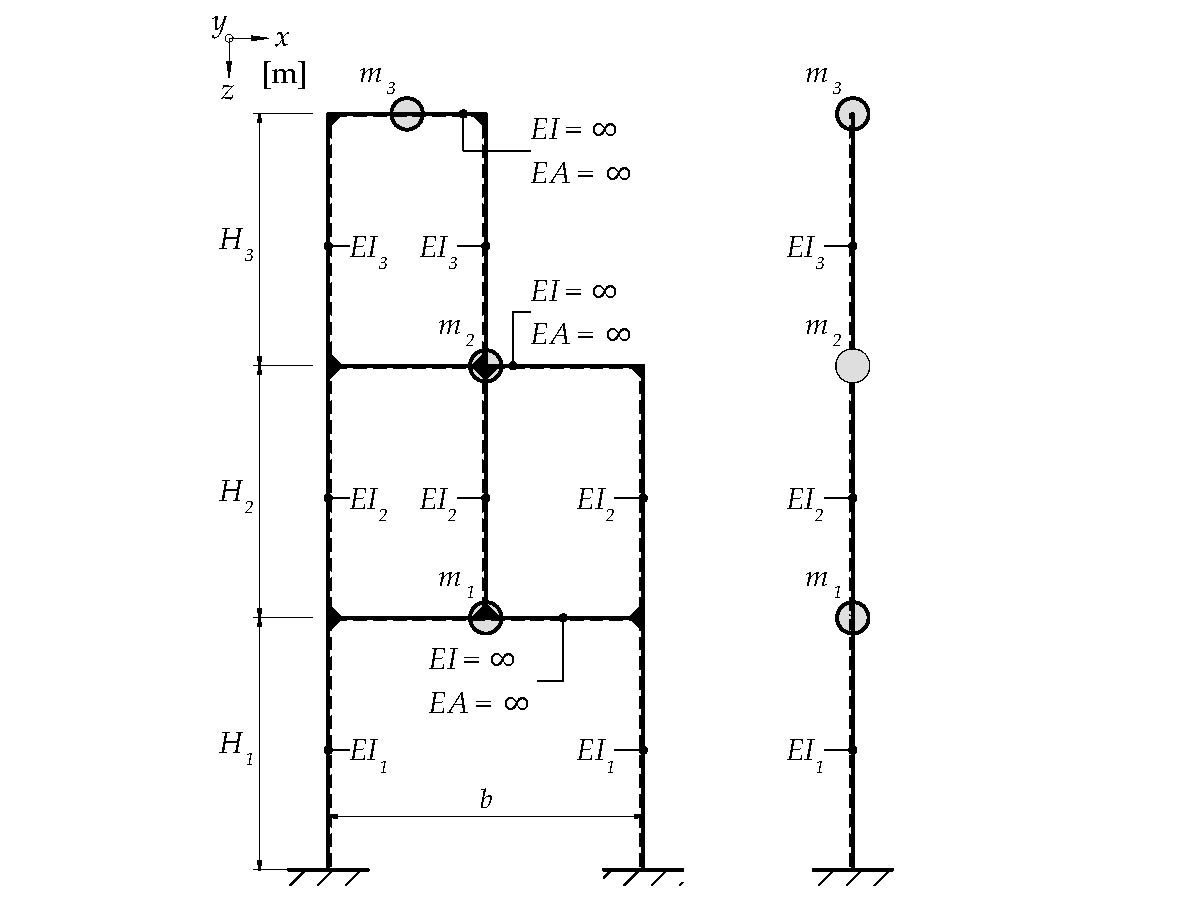
\includegraphics{index_files/mediabag/bilder/aufgabe_mms_3er_system.pdf}

}

\caption{\label{fig-mms_3er_system}Statisches System des
dreigeschossigen Gebäude}

\end{figure}

Gesucht:

\begin{itemize}
\tightlist
\item
  Bestimme die Steifigkeits- und Massenmatrix
\item
  Bestimme die Eigenkreisfrequenzen
\item
  Ermittle die daraus resultierenden Eigenvektoren
\item
  Führe eine modale Analyse durch

  \begin{itemize}
  \tightlist
  \item
    Kontrolliere die Orthogonalität der transformierten Matrizen
  \item
    Bestimme die Partizipationsfaktoren
  \end{itemize}
\item
  Ermittle die Pseudobeschleunigung anhand des Antwortspektrums der
  SIA261:2020
\item
  Ermittle die daraus resultierende Deformationen (Überlagere mittels
  SRSS-Regel)
\item
  Zeichne die maximalen Schnittkraftverläufe
\end{itemize}

Gegeben:

\begin{itemize}
\tightlist
\item
  Baugrundklasse \(E\)
\item
  Erdbebenzone \(Z2\)
\end{itemize}

\hypertarget{tbl-parameter_mms6}{}
\begin{longtable}[]{@{}
  >{\raggedright\arraybackslash}p{(\columnwidth - 2\tabcolsep) * \real{0.5000}}
  >{\raggedright\arraybackslash}p{(\columnwidth - 2\tabcolsep) * \real{0.5000}}@{}}
\caption{\label{tbl-parameter_mms6}Parameter der Aufgabe}\tabularnewline
\toprule\noalign{}
\endfirsthead
\endhead
\bottomrule\noalign{}
\endlastfoot
\(EI_{1} = 1150000.0 \text{m}^{2} \text{N}\) &
\(EI_{2} = 766666.0 \text{m}^{2} \text{N}\) \\
\(EI_{3} = 1150000.0 \text{m}^{2} \text{N}\) &
\(H_{1} = 4.5 \text{m}\) \\
\(H_{2} = 3.5 \text{m}\) & \(H_{3} = 3.5 \text{m}\) \\
\(m_{1} = \frac{5000 \text{N} \text{s}^{2}}{\text{m}}\) &
\(m_{2} = \frac{4000 \text{N} \text{s}^{2}}{\text{m}}\) \\
\(m_{3} = \frac{4000 \text{N} \text{s}^{2}}{\text{m}}\) & \\
\end{longtable}

\newpage{}

\hypertarget{musterluxf6sung-10}{%
\section{Musterlösung}\label{musterluxf6sung-10}}

\hypertarget{massenmatrix-m}{%
\subsection{\texorpdfstring{Massenmatrix
\(M\)}{Massenmatrix M}}\label{massenmatrix-m}}

\begin{figure}[H]

{\centering 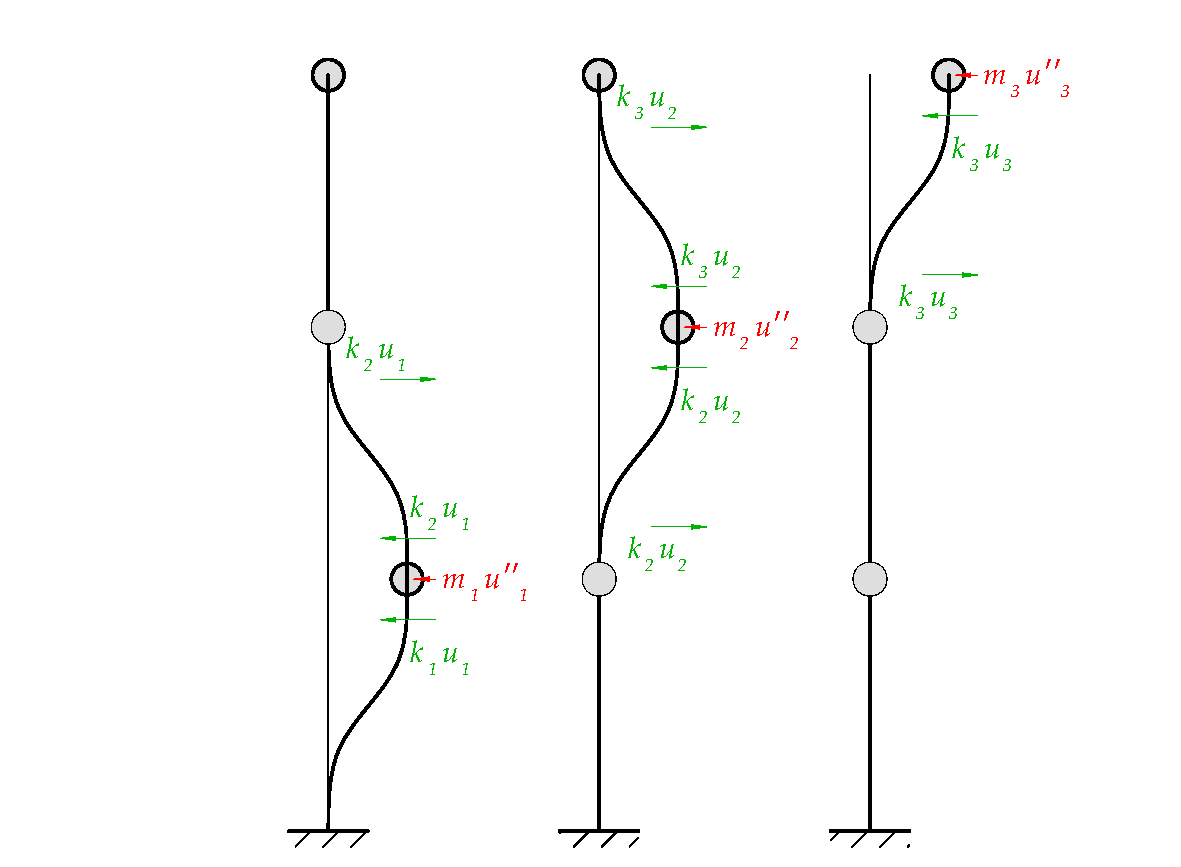
\includegraphics{index_files/mediabag/bilder/aufgabe_mms_3er_auslenk.pdf}

}

\caption{\label{fig-mms_3er_steifigkeit}Auslenkung der Massen zur
Ermittlung der Matrizen}

\end{figure}

\begin{equation}M = \left[\begin{matrix}m_{1} & 0 & 0\\0 & m_{2} & 0\\0 & 0 & m_{3}\end{matrix}\right]\end{equation}

\begin{equation}M = \left[\begin{matrix}\frac{5000 \text{N} \text{s}^{2}}{\text{m}} & 0 & 0\\0 & \frac{4000 \text{N} \text{s}^{2}}{\text{m}} & 0\\0 & 0 & \frac{4000 \text{N} \text{s}^{2}}{\text{m}}\end{matrix}\right]\end{equation}

\hypertarget{steifigkeitsmatrix-k}{%
\subsection{\texorpdfstring{Steifigkeitsmatrix
\(K\)}{Steifigkeitsmatrix K}}\label{steifigkeitsmatrix-k}}

\hypertarget{steifigkeit-der-stockwerke}{%
\subsubsection{Steifigkeit der
Stockwerke}\label{steifigkeit-der-stockwerke}}

\begin{equation}k_{1} = \frac{24 EI_{1}}{H_{1}^{3}}\end{equation}

\begin{equation}k_{1} = \frac{3.03 \cdot 10^{5} \text{N}}{\text{m}}\end{equation}

\begin{equation}k_{2} = \frac{36 EI_{2}}{H_{2}^{3}}\end{equation}

\begin{equation}k_{2} = \frac{6.44 \cdot 10^{5} \text{N}}{\text{m}}\end{equation}

\begin{equation}k_{3} = \frac{24 EI_{3}}{H_{3}^{3}}\end{equation}

\begin{equation}k_{3} = \frac{6.44 \cdot 10^{5} \text{N}}{\text{m}}\end{equation}

Abgefüllt in die Steifigkeitsmatrix

\begin{equation}K = \left[\begin{matrix}k_{1} + k_{2} & - k_{2} & 0\\- k_{2} & k_{2} + k_{3} & - k_{3}\\0 & - k_{3} & k_{3}\end{matrix}\right]\end{equation}

\begin{equation}K = \left[\begin{matrix}\frac{24 EI_{1}}{H_{1}^{3}} + \frac{36 EI_{2}}{H_{2}^{3}} & - \frac{36 EI_{2}}{H_{2}^{3}} & 0\\- \frac{36 EI_{2}}{H_{2}^{3}} & \frac{36 EI_{2}}{H_{2}^{3}} + \frac{24 EI_{3}}{H_{3}^{3}} & - \frac{24 EI_{3}}{H_{3}^{3}}\\0 & - \frac{24 EI_{3}}{H_{3}^{3}} & \frac{24 EI_{3}}{H_{3}^{3}}\end{matrix}\right]\end{equation}

\begin{equation}K = \left[\begin{matrix}\frac{9.47 \cdot 10^{5} \text{N}}{\text{m}} & - \frac{6.44 \cdot 10^{5} \text{N}}{\text{m}} & 0\\- \frac{6.44 \cdot 10^{5} \text{N}}{\text{m}} & \frac{1.29 \cdot 10^{6} \text{N}}{\text{m}} & - \frac{6.44 \cdot 10^{5} \text{N}}{\text{m}}\\0 & - \frac{6.44 \cdot 10^{5} \text{N}}{\text{m}} & \frac{6.44 \cdot 10^{5} \text{N}}{\text{m}}\end{matrix}\right]\end{equation}

\hypertarget{eigenvektoren-3}{%
\subsection{Eigenvektoren}\label{eigenvektoren-3}}

\hypertarget{eigenkreisfrequenzen-4}{%
\subsubsection{Eigenkreisfrequenzen}\label{eigenkreisfrequenzen-4}}

Bei einem Mehrmassenschwinger gibt es entsprechend den Freiheitsgraden
Eigenkreisfrequenzen \(\omega_n\). Diese lassen sich anhand folgender
Gleichung bestimmen:

\begin{equation}\protect\hypertarget{eq-mms_3er_eigenkreisfreqs}{}{
\det{[\mathbf{K}-\omega_n^2 \mathbf{M}]=0}
}\label{eq-mms_3er_eigenkreisfreqs}\end{equation}

\begin{equation}\omega_{1} = \frac{4.31}{\text{s}}\end{equation}

\begin{equation}\omega_{2} = \frac{13.3}{\text{s}}\end{equation}

\begin{equation}\omega_{3} = \frac{21.8}{\text{s}}\end{equation}

\begin{figure}[H]

{\centering 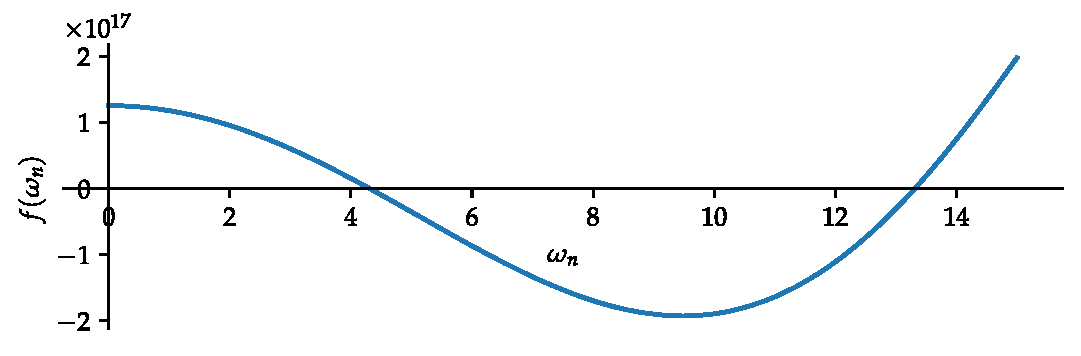
\includegraphics{index_files/mediabag/mms_04_files/figure-pdf/fig-loesung_eigenkreisfrequenzen-output-1.pdf}

}

\caption{\label{fig-loesung_eigenkreisfrequenzen}Nullstellen der
Gleichung~\ref{eq-mms_3er_eigenkreisfreqs}}

\end{figure}

\hypertarget{eigenvektoren-phi-2}{%
\subsubsection{\texorpdfstring{Eigenvektoren
\(\phi\)}{Eigenvektoren \textbackslash phi}}\label{eigenvektoren-phi-2}}

Durch das Einsetzen der bestimmten Eigenkreisfrequenzen lassen sich die
Eigenvektoren bestimmen. Die Einträge des Eigenvektors sind voneinander
abhängig und lassen sich dem entsprechen beliebig definieren.
Grundsätzlich wird der maximale Eigenwert zu \(1\) gesetzt.

\begin{equation}\protect\hypertarget{eq-mms_3er_mms_3_eigenvek}{}{
\mathbf{K} - \omega_n^2 \mathbf{M} \phi_n= 0
}\label{eq-mms_3er_mms_3_eigenvek}\end{equation}

\begin{equation}\phi_{1} = \left[\begin{matrix}0.667\\0.885\\1.0\end{matrix}\right]\end{equation}

\begin{equation}\phi_{2} = \left[\begin{matrix}1.0\\0.0933\\-0.916\end{matrix}\right]\end{equation}

\begin{equation}\phi_{3} = \left[\begin{matrix}0.449\\-1.0\\0.51\end{matrix}\right]\end{equation}

\hypertarget{modale-analyse-1}{%
\subsection{Modale Analyse}\label{modale-analyse-1}}

Die Modale Analyse zielt darauf ab, den Mehrmassenschwinger zu
entkoppeln. Dazu wird in einem ersten Schritt die
Orthogonalitätsbedingung kontrolliert. Diese muss erfüllt sein um eine
Entkoppelung durchzuführen. Siehe Kapitel~\ref{sec-mms_nach_ortho} für
eine ausführliche Erklärung.

\hypertarget{orthogonalituxe4tsbedingung-2}{%
\subsubsection{Orthogonalitätsbedingung}\label{orthogonalituxe4tsbedingung-2}}

Angewendet auf die Massenmatrix: Es zeigen sich kleine numerische
Unreinheiten, welche vernachlässigt werden können.

\begin{equation}\phi_{1}^{T} M \phi_{1} = \left[\begin{matrix}\frac{9.35 \cdot 10^{3} \text{N} \text{s}^{2}}{\text{m}}\end{matrix}\right]\end{equation}

\begin{equation}\phi_{2}^{T} M \phi_{1} = \left[\begin{matrix}- \frac{6.37 \cdot 10^{-12} \text{N} \text{s}^{2}}{\text{m}}\end{matrix}\right]\end{equation}

\begin{equation}\phi_{3}^{T} M \phi_{1} = \left[\begin{matrix}- \frac{3.18 \cdot 10^{-12} \text{N} \text{s}^{2}}{\text{m}}\end{matrix}\right]\end{equation}

\begin{equation}\phi_{1}^{T} M \phi_{2} = \left[\begin{matrix}- \frac{6.37 \cdot 10^{-12} \text{N} \text{s}^{2}}{\text{m}}\end{matrix}\right]\end{equation}

\begin{equation}\phi_{2}^{T} M \phi_{2} = \left[\begin{matrix}\frac{8.39 \cdot 10^{3} \text{N} \text{s}^{2}}{\text{m}}\end{matrix}\right]\end{equation}

\begin{equation}\phi_{3}^{T} M \phi_{2} = \left[\begin{matrix}\frac{1.8 \cdot 10^{-11} \text{N} \text{s}^{2}}{\text{m}}\end{matrix}\right]\end{equation}

\begin{equation}\phi_{1}^{T} M \phi_{3} = \left[\begin{matrix}- \frac{3.18 \cdot 10^{-12} \text{N} \text{s}^{2}}{\text{m}}\end{matrix}\right]\end{equation}

\begin{equation}\phi_{2}^{T} M \phi_{3} = \left[\begin{matrix}\frac{1.8 \cdot 10^{-11} \text{N} \text{s}^{2}}{\text{m}}\end{matrix}\right]\end{equation}

\begin{equation}\phi_{3}^{T} M \phi_{3} = \left[\begin{matrix}\frac{6.05 \cdot 10^{3} \text{N} \text{s}^{2}}{\text{m}}\end{matrix}\right]\end{equation}

Für die Steifigkeitsmatrix:

\begin{equation}\phi_{1}^{T} K \phi_{1} = \left[\begin{matrix}\frac{1.74 \cdot 10^{5} \text{N}}{\text{m}}\end{matrix}\right]\end{equation}

\begin{equation}\phi_{2}^{T} K \phi_{1} = \left[\begin{matrix}- \frac{6.4 \cdot 10^{-10} \text{N}}{\text{m}}\end{matrix}\right]\end{equation}

\begin{equation}\phi_{3}^{T} K \phi_{1} = \left[\begin{matrix}- \frac{6.55 \cdot 10^{-11} \text{N}}{\text{m}}\end{matrix}\right]\end{equation}

\begin{equation}\phi_{1}^{T} K \phi_{2} = \left[\begin{matrix}- \frac{6.4 \cdot 10^{-10} \text{N}}{\text{m}}\end{matrix}\right]\end{equation}

\begin{equation}\phi_{2}^{T} K \phi_{2} = \left[\begin{matrix}\frac{1.49 \cdot 10^{6} \text{N}}{\text{m}}\end{matrix}\right]\end{equation}

\begin{equation}\phi_{3}^{T} K \phi_{2} = \left[\begin{matrix}\frac{3.73 \cdot 10^{-9} \text{N}}{\text{m}}\end{matrix}\right]\end{equation}

\begin{equation}\phi_{1}^{T} K \phi_{3} = \left[\begin{matrix}- \frac{6.55 \cdot 10^{-11} \text{N}}{\text{m}}\end{matrix}\right]\end{equation}

\begin{equation}\phi_{2}^{T} K \phi_{3} = \left[\begin{matrix}\frac{3.73 \cdot 10^{-9} \text{N}}{\text{m}}\end{matrix}\right]\end{equation}

\begin{equation}\phi_{3}^{T} K \phi_{3} = \left[\begin{matrix}\frac{2.88 \cdot 10^{6} \text{N}}{\text{m}}\end{matrix}\right]\end{equation}

\hypertarget{modal--und-spektralmatrix-1}{%
\subsubsection{Modal- und
Spektralmatrix}\label{modal--und-spektralmatrix-1}}

Mittels der Modal- und Spektralmatrix lassen sich die generalisierten
Grössen effizient ermitteln.

\begin{equation}Modalmatrix = \Phi\end{equation}

\begin{equation}\Phi = \left[\begin{matrix}0.667 & 1.0 & 0.4487\\0.8846 & 0.09327 & -1.0\\1.0 & -0.9162 & 0.5104\end{matrix}\right]\end{equation}

\begin{equation}Spektralmatrix = \Omega^{2}\end{equation}

\begin{equation}\Omega^{2} = \left[\begin{matrix}\frac{18.58}{\text{s}^{2}} & 0 & 0\\0 & \frac{177.3}{\text{s}^{2}} & 0\\0 & 0 & \frac{476.2}{\text{s}^{2}}\end{matrix}\right]\end{equation}

\hypertarget{generalisierte-gruxf6ssen-1}{%
\subsubsection{Generalisierte
Grössen}\label{generalisierte-gruxf6ssen-1}}

Zur Reduktion des Rechenaufwands werden die numerischen Unreinheiten zu
Null gesetzt.

\begin{equation}M^{\star} = \left[\begin{matrix}\frac{9354.1 \text{N} \text{s}^{2}}{\text{m}} & 0 & 0\\0 & \frac{8392.7 \text{N} \text{s}^{2}}{\text{m}} & 0\\0 & 0 & \frac{6049.0 \text{N} \text{s}^{2}}{\text{m}}\end{matrix}\right]\end{equation}

\begin{equation}K^{\star} = \left[\begin{matrix}\frac{1.7379 \cdot 10^{5} \text{N}}{\text{m}} & 0 & 0\\0 & \frac{1.4881 \cdot 10^{6} \text{N}}{\text{m}} & 0\\0 & 0 & \frac{2.8807 \cdot 10^{6} \text{N}}{\text{m}}\end{matrix}\right]\end{equation}

\hypertarget{modale-huxf6hen-1}{%
\subsubsection{Modale Höhen}\label{modale-huxf6hen-1}}

Die modalen Höhen bestimmen sich aus
Gleichung~\ref{eq-mms_3er_modale_hoehe}:

\begin{equation}\protect\hypertarget{eq-mms_3er_modale_hoehe}{}{
H_n = \frac{L_n^\theta}{L_n}
}\label{eq-mms_3er_modale_hoehe}\end{equation}

\begin{equation}\protect\hypertarget{eq-mms_3er_L_n}{}{
L_n = \phi_n^T \cdot \mathbf{M 1}
}\label{eq-mms_3er_L_n}\end{equation}

\begin{equation}\protect\hypertarget{eq-mms_3er_L_n_theta}{}{
L_n^\theta = \sum_{j=1}^N H_j \cdot m_j \cdot \phi_{jn}
}\label{eq-mms_3er_L_n_theta}\end{equation}

Angewendet auf das Beispiel folgt:

\begin{equation}H = \left[\begin{matrix}H_{1}\\H_{2}\\H_{3}\end{matrix}\right]\end{equation}

\begin{equation}H = \left[\begin{matrix}\frac{H_{1} m_{1} \phi_{11} + H_{2} m_{2} \phi_{21} + H_{3} m_{3} \phi_{31}}{m_{1} \phi_{11} + m_{1} \phi_{21} + m_{1} \phi_{31}}\\\frac{H_{1} m_{1} \phi_{12} + H_{2} m_{2} \phi_{22} + H_{3} m_{3} \phi_{32}}{m_{2} \phi_{12} + m_{2} \phi_{22} + m_{2} \phi_{32}}\\\frac{H_{1} m_{1} \phi_{13} + H_{2} m_{2} \phi_{23} + H_{3} m_{3} \phi_{33}}{m_{3} \phi_{13} + m_{3} \phi_{23} + m_{3} \phi_{33}}\end{matrix}\right]\end{equation}

\begin{equation}H = \left[\begin{matrix}3.24 \text{m}\\15.5 \text{m}\\- 19.9 \text{m}\end{matrix}\right]\end{equation}

Modalen Höhen kleiner als null sind zu vernachlässigen.

\hypertarget{kontrolle-der-modalen-transformation-1}{%
\subsubsection{Kontrolle der modalen
Transformation}\label{kontrolle-der-modalen-transformation-1}}

Die Eigenkreisfrequenzen ändern sich durch die Transformation nicht.

\begin{equation}\omega_{1} = \frac{4.31}{\text{s}}\end{equation}

\begin{equation}\omega_{1 modal} = \frac{4.31}{\text{s}}\end{equation}

\begin{equation}\omega_{2} = \frac{13.32}{\text{s}}\end{equation}

\begin{equation}\omega_{2 modal} = \frac{13.32}{\text{s}}\end{equation}

\begin{equation}\omega_{3} = \frac{21.82}{\text{s}}\end{equation}

\begin{equation}\omega_{3 modal} = \frac{21.82}{\text{s}}\end{equation}

\hypertarget{partizipationsfaktor-gamma}{%
\subsubsection{\texorpdfstring{Partizipationsfaktor
\(\Gamma\)}{Partizipationsfaktor \textbackslash Gamma}}\label{partizipationsfaktor-gamma}}

Die Verteilung des Partizipationsfaktor gibt einen direkten Hinweis,
welcher Eigenmode an der Gesamtanwort den grössten Einfluss (beteiligt
bzw. partizipiert) hat.

\begin{equation}\protect\hypertarget{eq-mms_3er_part}{}{
\Gamma_n = \frac{\Phi_n^T \mathbf{M 1}}{\Phi_n^T \mathbf{M}\Phi_n}
}\label{eq-mms_3er_part}\end{equation}

In allgemeiner Form lautet der Partizipationsfaktor:

\begin{equation}\protect\hypertarget{eq-mms_3er_split_part}{}{
\Gamma_n = \frac{\Phi_n^T \mathbf{M r^\star}}{\Phi_n^T \mathbf{M}\Phi_n}
}\label{eq-mms_3er_split_part}\end{equation}

\(\mathbf{r^\star}\) beschreibt die Starrkörperverschiebung infolge der
Erdbebenanregung \(u_g\) am Fusspunkt des Gesamtsystems.

\begin{equation}\protect\hypertarget{eq-mms_3er_starrkoerperverschiebung}{}{
\mathbf{r^\star} = \begin{bmatrix}
FHG_1 \\
FHG_2 
\end{bmatrix}=
\begin{bmatrix}
\cos(0) \\
\cos(0) 
\end{bmatrix}=
\begin{bmatrix}
1 \\
1 
\end{bmatrix}= \mathbf{1}
}\label{eq-mms_3er_starrkoerperverschiebung}\end{equation}

Die Partizipationsmatrix lässt sich direkt durch folgende Gleichung
ermitteln:

\begin{equation}\protect\hypertarget{eq-mms_3er_matrix_part}{}{
\Gamma = M^{\star-1} \cdot \Phi^T \cdot M \cdot 1
}\label{eq-mms_3er_matrix_part}\end{equation}

Gelöst mit Gleichung~\ref{eq-mms_3er_matrix_part}:

\begin{equation}\Gamma = \left[\begin{matrix}1.16\\0.204\\0.0472\end{matrix}\right]\end{equation}

Gelöst mit Gleichung~\ref{eq-mms_3er_split_part}:

\begin{equation}\Gamma_{1} = \frac{m_{1} \phi_{11} + m_{2} \phi_{21} + m_{3} \phi_{31}}{m_{1} \phi_{11}^{2} + m_{2} \phi_{21}^{2} + m_{3} \phi_{31}^{2}}\end{equation}

\begin{equation}\Gamma_{1} = 1.16\end{equation}

\begin{equation}\Gamma_{2} = \frac{m_{1} \phi_{12} + m_{2} \phi_{22} + m_{3} \phi_{32}}{m_{1} \phi_{12}^{2} + m_{2} \phi_{22}^{2} + m_{3} \phi_{32}^{2}}\end{equation}

\begin{equation}\Gamma_{2} = 0.204\end{equation}

\begin{equation}\Gamma_{3} = \frac{m_{1} \phi_{13} + m_{2} \phi_{23} + m_{3} \phi_{33}}{m_{1} \phi_{13}^{2} + m_{2} \phi_{23}^{2} + m_{3} \phi_{33}^{2}}\end{equation}

\begin{equation}\Gamma_{3} = 0.0472\end{equation}

\begin{figure}[H]

{\centering \includegraphics{index_files/mediabag/mms_04_files/figure-pdf/fig-mms_3_modale_ems-output-1.pdf}

}

\caption{\label{fig-mms_3_modale_ems}Darstellung der entkoppelten
Einmassenschwinger}

\end{figure}

\hypertarget{elastisches-antwortspektrum}{%
\subsection{Elastisches
Antwortspektrum}\label{elastisches-antwortspektrum}}

Aus der Aufgabenstellung darf nach
(\protect\hyperlink{ref-SIA261_2020}{Schweizerischer Ingenieur- und
Architektenverein (SIA), 2020}) Abs. 16.2.3.1 Kurve \(E\) gewählt
werden.

\hypertarget{grundschwingzeit}{%
\subsubsection{Grundschwingzeit}\label{grundschwingzeit}}

Die Grundschwingzeit kann anhand der bereits ermittelten
Eigenkreisfrequenzen ermittelt werden.

\begin{equation}\protect\hypertarget{eq-mms_3er_eigenperiode}{}{
T = \frac{2 \pi}{\omega}
}\label{eq-mms_3er_eigenperiode}\end{equation}

\begin{equation}T_{1} = 1.46 \text{s}\end{equation}

\begin{equation}T_{2} = 0.472 \text{s}\end{equation}

\begin{equation}T_{3} = 0.288 \text{s}\end{equation}

\hypertarget{elastisches-antwortspektrum-1}{%
\subsubsection{Elastisches
Antwortspektrum}\label{elastisches-antwortspektrum-1}}

Es wird für sämtliche Eigenperioden die Pseudobeschleunigung bestimmt.
Siehe dazu Schweizerischer Ingenieur- und Architektenverein (SIA)
(\protect\hyperlink{ref-SIA261_2020}{2020}).

\begin{longtable}[]{@{}
  >{\raggedright\arraybackslash}p{(\columnwidth - 2\tabcolsep) * \real{0.5000}}
  >{\raggedright\arraybackslash}p{(\columnwidth - 2\tabcolsep) * \real{0.5000}}@{}}
\toprule\noalign{}
\endhead
\bottomrule\noalign{}
\endlastfoot
\(S = 1.7\) & \(T_{B} = 0.1 \text{s}\) \\
\(T_{C} = 0.5 \text{s}\) & \(T_{D} = 2.0 \text{s}\) \\
\(\eta = 1\) & \\
\end{longtable}

\begin{equation}S_{e} = \frac{2.5 S_{} T_{C} a_{gd} \eta}{T}\end{equation}

\begin{equation}S_{e 1} = \frac{1.46 \text{m}}{\text{s}^{2}}\end{equation}

\begin{longtable}[]{@{}
  >{\raggedright\arraybackslash}p{(\columnwidth - 2\tabcolsep) * \real{0.5000}}
  >{\raggedright\arraybackslash}p{(\columnwidth - 2\tabcolsep) * \real{0.5000}}@{}}
\toprule\noalign{}
\endhead
\bottomrule\noalign{}
\endlastfoot
\(S = 1.7\) & \(T_{B} = 0.1 \text{s}\) \\
\(T_{C} = 0.5 \text{s}\) & \(T_{D} = 2.0 \text{s}\) \\
\(\eta = 1\) & \\
\end{longtable}

\begin{equation}S_{e} = 2.5 S_{} a_{gd} \eta\end{equation}

\begin{equation}S_{e 2} = \frac{4.25 \text{m}}{\text{s}^{2}}\end{equation}

\begin{longtable}[]{@{}
  >{\raggedright\arraybackslash}p{(\columnwidth - 2\tabcolsep) * \real{0.5000}}
  >{\raggedright\arraybackslash}p{(\columnwidth - 2\tabcolsep) * \real{0.5000}}@{}}
\toprule\noalign{}
\endhead
\bottomrule\noalign{}
\endlastfoot
\(S = 1.7\) & \(T_{B} = 0.1 \text{s}\) \\
\(T_{C} = 0.5 \text{s}\) & \(T_{D} = 2.0 \text{s}\) \\
\(\eta = 1\) & \\
\end{longtable}

\begin{equation}S_{e} = 2.5 S_{} a_{gd} \eta\end{equation}

\begin{equation}S_{e 3} = \frac{4.25 \text{m}}{\text{s}^{2}}\end{equation}

\hypertarget{maximale-deformation}{%
\subsection{Maximale Deformation}\label{maximale-deformation}}

Die maximale Deformation resultiert aus der Beschleunigung \(S_e\) und
der Eigenkreisfrequenz \(\omega_n^2\). Für die Modalen EMS gilt es diese
anhand der Partizipationsfaktoren zu gewichten. Zur effektiven
Bestimmung der Auslenkung sind die Resultate der EMS mittels SRSS-Regel
zu überlagern.

\begin{equation}q_{1 max} = \frac{\Gamma_{1} S_{e 1}}{\omega_{1}^{2}}\end{equation}

\begin{equation}q_{1 max} = 0.0912 \text{m}\end{equation}

\begin{equation}q_{2 max} = \frac{\Gamma_{2} S_{e 2}}{\omega_{2}^{2}}\end{equation}

\begin{equation}q_{2 max} = 0.00488 \text{m}\end{equation}

\begin{equation}q_{3 max} = \frac{\Gamma_{3} S_{e 3}}{\omega_{3}^{2}}\end{equation}

\begin{equation}q_{3 max} = 0.000421 \text{m}\end{equation}

Um die Entkoppelung rückzuführen gilt es die erhaltenen Resultate zu
überlagern. Dabei gibt es unterschiedliche Ansätze. Bei weit auseinander
liegenden Eigenfrequenzen kann die SRSS-Überlagerung (Square-root of the
sum of squares) verwendet werden.

\begin{equation}\protect\hypertarget{eq-mms_3er_srss}{}{
u_{max} = \sqrt{\sum_{n=1}^2 (q_{n} \cdot \phi_n)^2}
}\label{eq-mms_3er_srss}\end{equation}

\begin{equation}u_{max} = \left[\begin{matrix}0.061 \text{m}\\0.0807 \text{m}\\0.0913 \text{m}\end{matrix}\right]\end{equation}

\ul{Stephan, wieso multiplizierst du die SRSS- Überlagerung nochmals
mit} \(phi_1\)

\begin{figure}[H]

{\centering \includegraphics{bilder/Frage_1.png}

}

\caption{Frage}

\end{figure}

\hypertarget{maximale-schnittkruxe4fte}{%
\subsection{Maximale Schnittkräfte}\label{maximale-schnittkruxe4fte}}

\hypertarget{querkruxe4fte}{%
\subsubsection{Querkräfte}\label{querkruxe4fte}}

Die Einwirkungen resultieren aus der Masse multipliziert mit der
Beschleunigung aus dem Antwortspektrum. Dazu sind in einem ersten
Schritt die beiden entkoppelten EMS von einander getrennt zu betrachten.
Die Überlagerung erfolgt erst bei den ermittelten Querkräften.

\begin{equation}\protect\hypertarget{eq-mms_3er_masse}{}{
m_1 = \Gamma \cdot M \cdot \phi_1
}\label{eq-mms_3er_masse}\end{equation}

\begin{equation}\protect\hypertarget{eq-mms_3er_kraft_aus_masse}{}{
F_{1max} = m_1 \cdot S_{e1}
}\label{eq-mms_3er_kraft_aus_masse}\end{equation}

Aus dem ersten EMS folgt:

\begin{equation}m_{1} = \left[\begin{matrix}\frac{3876.5 \text{N} \text{s}^{2}}{\text{m}}\\\frac{4112.8 \text{N} \text{s}^{2}}{\text{m}}\\\frac{4649.6 \text{N} \text{s}^{2}}{\text{m}}\end{matrix}\right]\end{equation}

\begin{equation}F_{1 max} = \left[\begin{matrix}5652.3 \text{N}\\5996.8 \text{N}\\6779.5 \text{N}\end{matrix}\right]\end{equation}

\begin{equation}V_{1} = \left[\begin{matrix}18429.0 \text{N}\\12776.0 \text{N}\\6779.5 \text{N}\end{matrix}\right]\end{equation}

Aus dem zweiten EMS folglich:

\begin{equation}m_{2} = \left[\begin{matrix}\frac{1017.6 \text{N} \text{s}^{2}}{\text{m}}\\\frac{75.929 \text{N} \text{s}^{2}}{\text{m}}\\- \frac{745.91 \text{N} \text{s}^{2}}{\text{m}}\end{matrix}\right]\end{equation}

\begin{equation}F_{2 max} = \left[\begin{matrix}4325.0 \text{N}\\322.7 \text{N}\\- 3170.1 \text{N}\end{matrix}\right]\end{equation}

\begin{equation}V_{2} = \left[\begin{matrix}1477.5 \text{N}\\- 2847.4 \text{N}\\- 3170.1 \text{N}\end{matrix}\right]\end{equation}

Aus dem dritten EMS folglich:

\begin{equation}m_{3} = \left[\begin{matrix}\frac{105.86 \text{N} \text{s}^{2}}{\text{m}}\\- \frac{188.73 \text{N} \text{s}^{2}}{\text{m}}\\\frac{96.33 \text{N} \text{s}^{2}}{\text{m}}\end{matrix}\right]\end{equation}

\begin{equation}F_{3 max} = \left[\begin{matrix}449.91 \text{N}\\- 802.09 \text{N}\\409.4 \text{N}\end{matrix}\right]\end{equation}

\begin{equation}V_{3} = \left[\begin{matrix}57.229 \text{N}\\- 392.69 \text{N}\\409.4 \text{N}\end{matrix}\right]\end{equation}

Maximale Querkraft aus Überlagerung beider EMS mittels SRSS-Regel.

\begin{equation}\protect\hypertarget{eq-mms_3er_max_querkraft}{}{
V_{max} = \sqrt{V_1^2 + V_2^2 + V_3^2}
}\label{eq-mms_3er_max_querkraft}\end{equation}

\begin{equation}V_{max} = \left[\begin{matrix}1.85 \cdot 10^{4} \text{N}\\1.31 \cdot 10^{4} \text{N}\\7.5 \cdot 10^{3} \text{N}\end{matrix}\right]\end{equation}

\hypertarget{biegemomente}{%
\subsubsection{Biegemomente}\label{biegemomente}}

Die Biegemomente lassen sich abschliessend anhand der Querkräfte
bestimmen.

\hypertarget{normalkruxe4fte}{%
\subsubsection{Normalkräfte}\label{normalkruxe4fte}}

Die Normalkräfte resultieren aus den Punktmassen.

\begin{figure}[H]

{\centering \includegraphics{index_files/mediabag/mms_04_files/figure-pdf/fig-schnittgroessen-output-1.pdf}

}

\caption{\label{fig-schnittgroessen}Maximale Schnittgrössen}

\end{figure}

\hypertarget{beispiel-antwortspektrenverfahren-an-einem-rahmen}{%
\chapter{Beispiel: Antwortspektrenverfahren an einem
Rahmen}\label{beispiel-antwortspektrenverfahren-an-einem-rahmen}}

\hypertarget{aufgabenstellung-13}{%
\section{Aufgabenstellung}\label{aufgabenstellung-13}}

Dies ist eine Weiterführung des bereits bekannten Rahmentragwerks aus
Kapitel~\ref{sec-mms_steif}.

\begin{figure}[H]

{\centering \includegraphics{index_files/mediabag/bilder/aufgabe_mms_steif_system.pdf}

}

\caption{\label{fig-mms_antwort_system_mms2}Statisches System des
Rahmentragwerks}

\end{figure}

Gesucht:

\begin{itemize}
\item
  Eigenkreisfrequenz \(\omega\)
\item
  Eigenformen - Normierung auf \[\phi_1^T = 
  \begin{bmatrix}
   &  1\\
  \end{bmatrix} \] \[\phi_2^T =
  \begin{bmatrix}
   &  1\\
  \end{bmatrix}\]
\item
  Skizze der Eigenformen
\item
  Statische Ersatzkräfte mit elastischem Antwortspektrum aus
  (\protect\hyperlink{ref-SIA261_2020}{Schweizerischer Ingenieur- und
  Architektenverein (SIA), 2020}) Abs. 16.2.3 auf Stockwerksebene.
  Überlagerung mit der SRSS-Methode.
\end{itemize}

Gegeben:

\begin{itemize}
\tightlist
\item
  Dehnsteifigkeit aller Stäbe \(E\cdot A = \infty\)
\item
  Baugrundklasse B
\item
  Erdbebenzone Z2
\end{itemize}

\hypertarget{tbl-parameter_mms5}{}
\begin{longtable}[]{@{}
  >{\raggedright\arraybackslash}p{(\columnwidth - 2\tabcolsep) * \real{0.5000}}
  >{\raggedright\arraybackslash}p{(\columnwidth - 2\tabcolsep) * \real{0.5000}}@{}}
\caption{\label{tbl-parameter_mms5}Verwendete Parameter}\tabularnewline
\toprule\noalign{}
\endfirsthead
\endhead
\bottomrule\noalign{}
\endlastfoot
\(E = \frac{30000 \text{N}}{\text{mm}^{2}}\) & \(H = 3.2 \text{m}\) \\
\(I = 2000000000 \text{mm}^{4}\) &
\(m_{1} = \frac{40000 \text{N} \text{s}^{2}}{\text{m}}\) \\
\(m_{2} = \frac{20000 \text{N} \text{s}^{2}}{\text{m}}\) & \\
\end{longtable}

\newpage{}

\hypertarget{musterluxf6sung-11}{%
\section{Musterlösung}\label{musterluxf6sung-11}}

Die Lösung deckt sich mit Kapitel~\ref{sec-mms_steif_ML} bis zu den
ermittelten Eigenformen.

\hypertarget{steifigkeitsmatrix-mathbfk-1}{%
\subsection{\texorpdfstring{Steifigkeitsmatrix
\(\mathbf{K}\)}{Steifigkeitsmatrix \textbackslash mathbf\{K\}}}\label{steifigkeitsmatrix-mathbfk-1}}

\hypertarget{horizontale-steifigkeit-3}{%
\subsubsection{Horizontale
Steifigkeit}\label{horizontale-steifigkeit-3}}

\begin{equation}K = \left[\begin{matrix}k_{1} + k_{2} & - k_{2}\\- k_{2} & k_{2}\end{matrix}\right]\end{equation}

\begin{equation}K = \left[\begin{matrix}\frac{1.31836 \cdot 10^{8} \text{N}}{\text{m}} & - \frac{4.39453 \cdot 10^{7} \text{N}}{\text{m}}\\- \frac{4.39453 \cdot 10^{7} \text{N}}{\text{m}} & \frac{4.39453 \cdot 10^{7} \text{N}}{\text{m}}\end{matrix}\right]\end{equation}

\hypertarget{eigenvektoren-4}{%
\subsection{Eigenvektoren}\label{eigenvektoren-4}}

\hypertarget{massenmatrix-mathbfm-3}{%
\subsubsection{\texorpdfstring{Massenmatrix
\(\mathbf{M}\)}{Massenmatrix \textbackslash mathbf\{M\}}}\label{massenmatrix-mathbfm-3}}

\begin{equation}M = \left[\begin{matrix}m_{1} & 0\\0 & m_{2}\end{matrix}\right]\end{equation}

\begin{equation}M = \left[\begin{matrix}\frac{40000 \text{N} \text{s}^{2}}{\text{m}} & 0\\0 & \frac{20000 \text{N} \text{s}^{2}}{\text{m}}\end{matrix}\right]\end{equation}

\hypertarget{eigenkreisfrequenzen-5}{%
\subsubsection{Eigenkreisfrequenzen}\label{eigenkreisfrequenzen-5}}

\begin{equation}\omega_{1} = \frac{33.1}{\text{s}}\end{equation}

\begin{equation}\omega_{2} = \frac{66.3}{\text{s}}\end{equation}

\hypertarget{eigenvektoren-phi-3}{%
\subsubsection{\texorpdfstring{Eigenvektoren
\(\phi\)}{Eigenvektoren \textbackslash phi}}\label{eigenvektoren-phi-3}}

\begin{equation}\left[\begin{matrix}\frac{- k_{2} m_{2} \phi_{21} + \frac{\phi_{11} \left(- k_{2} m_{1} + m_{2} \left(k_{1} + k_{2}\right) + \sqrt{k_{1}^{2} m_{2}^{2} - 2 k_{1} k_{2} m_{1} m_{2} + 2 k_{1} k_{2} m_{2}^{2} + k_{2}^{2} m_{1}^{2} + 2 k_{2}^{2} m_{1} m_{2} + k_{2}^{2} m_{2}^{2}}\right)}{2}}{m_{2}}\\\frac{- k_{2} m_{1} \phi_{11} + \frac{\phi_{21} \left(k_{2} m_{1} - m_{2} \left(k_{1} + k_{2}\right) + \sqrt{k_{1}^{2} m_{2}^{2} - 2 k_{1} k_{2} m_{1} m_{2} + 2 k_{1} k_{2} m_{2}^{2} + k_{2}^{2} m_{1}^{2} + 2 k_{2}^{2} m_{1} m_{2} + k_{2}^{2} m_{2}^{2}}\right)}{2}}{m_{1}}\end{matrix}\right] = \left[\begin{matrix}0\\0\end{matrix}\right]\end{equation}

\begin{equation}\phi_{1} = \left[\begin{matrix}0.5\\1.0\end{matrix}\right]\end{equation}

\begin{equation}\left[\begin{matrix}\frac{- k_{2} m_{2} \phi_{22} + \frac{\phi_{12} \left(- k_{2} m_{1} + m_{2} \left(k_{1} + k_{2}\right) - \sqrt{k_{1}^{2} m_{2}^{2} - 2 k_{1} k_{2} m_{1} m_{2} + 2 k_{1} k_{2} m_{2}^{2} + k_{2}^{2} m_{1}^{2} + 2 k_{2}^{2} m_{1} m_{2} + k_{2}^{2} m_{2}^{2}}\right)}{2}}{m_{2}}\\\frac{- k_{2} m_{1} \phi_{12} + \frac{\phi_{22} \left(k_{2} m_{1} - m_{2} \left(k_{1} + k_{2}\right) - \sqrt{k_{1}^{2} m_{2}^{2} - 2 k_{1} k_{2} m_{1} m_{2} + 2 k_{1} k_{2} m_{2}^{2} + k_{2}^{2} m_{1}^{2} + 2 k_{2}^{2} m_{1} m_{2} + k_{2}^{2} m_{2}^{2}}\right)}{2}}{m_{1}}\end{matrix}\right] = \left[\begin{matrix}0\\0\end{matrix}\right]\end{equation}

\begin{equation}\phi_{2} = \left[\begin{matrix}-1.0\\1.0\end{matrix}\right]\end{equation}

\hypertarget{orthogonalituxe4tsbedingung-3}{%
\subsubsection{Orthogonalitätsbedingung}\label{orthogonalituxe4tsbedingung-3}}

\begin{equation}\phi_{1}^{T} M \phi_{1} = \left[\begin{matrix}\frac{3.0 \cdot 10^{4} \text{N} \text{s}^{2}}{\text{m}}\end{matrix}\right]\end{equation}

\begin{equation}\phi_{2}^{T} M \phi_{2} = \left[\begin{matrix}\frac{6.0 \cdot 10^{4} \text{N} \text{s}^{2}}{\text{m}}\end{matrix}\right]\end{equation}

\begin{equation}\phi_{2}^{T} M \phi_{1} = \left[\begin{matrix}0\end{matrix}\right]\end{equation}

\begin{equation}\phi_{1}^{T} M \phi_{2} = \left[\begin{matrix}0\end{matrix}\right]\end{equation}

Für die Steifigkeitsmatrix:

\begin{equation}\phi_{1}^{T} K \phi_{1} = \left[\begin{matrix}\frac{3.3 \cdot 10^{7} \text{N}}{\text{m}}\end{matrix}\right]\end{equation}

\begin{equation}\phi_{2}^{T} K \phi_{2} = \left[\begin{matrix}\frac{2.64 \cdot 10^{8} \text{N}}{\text{m}}\end{matrix}\right]\end{equation}

\begin{equation}\phi_{2}^{T} K \phi_{1} = \left[\begin{matrix}0\end{matrix}\right]\end{equation}

\begin{equation}\phi_{1}^{T} K \phi_{2} = \left[\begin{matrix}0\end{matrix}\right]\end{equation}

\hypertarget{eigenformen-2}{%
\subsubsection{Eigenformen}\label{eigenformen-2}}

\begin{figure}[H]

{\centering \includegraphics{index_files/mediabag/bilder/aufgabe_mms_steif_eigenvektoren.pdf}

}

\caption{\label{fig-mms_antwort_eigenformen}Die beiden Eigenformen
skizziert}

\end{figure}

\hypertarget{modale-analyse-2}{%
\subsection{Modale Analyse}\label{modale-analyse-2}}

Die Bewegungsgleichung für einen ungedämpften, frei schwingenden
Mehrmassenschwinger lässt sich folgend beschreiben:

\begin{equation}\protect\hypertarget{eq-mms_antwort_bewegungsgleichung}{}{
\mathbf{M u''(t) + K u = 0}
}\label{eq-mms_antwort_bewegungsgleichung}\end{equation}

Die Matrix-Gleichung beschreibt ein System aus Differentialgleichungen.
Die Modale Analyse zielt darauf ab, diese zu entkoppeln. Bezogen auf den
Mehrmassenschwinger heisst eine Entkoppelung, dass diese in
Einmassenschwinger aufgeteilt werden. Dies wird nun schrittweise
durchgeführt.

\hypertarget{modal--und-spektralmatrix-2}{%
\subsubsection{Modal- und
Spektralmatrix}\label{modal--und-spektralmatrix-2}}

Mittels der Modal- und Spektralmatrix können die generalisierten Grössen
ermittelt werden. Diese sind die eigenschaften der einzelnen
Einmassenschwinger. Die generalisierten Werte besitzen keine
physikalische Bedeutung, sie sind abhängig von der Wahl der
Eigenvektoren, welche bekanntlich von der Normierung abhängen.

Anhand der Bewegungsgleichung können die generalisierten Grössen
bestimmt werden, es gilt:

\begin{equation}\protect\hypertarget{eq-mms_ant_beweg_generalisiert}{}{
\Phi^T\mathbf{ M} \Phi \mathbf{u''(t)} + \Phi^T \mathbf{K} \Phi \mathbf{u(t)} = 0
}\label{eq-mms_ant_beweg_generalisiert}\end{equation}

\begin{equation}\protect\hypertarget{eq-mms_ant_beweg_generalisiert_subs}{}{
\mathbf{M^*u''(t) + K^* u(t) = 0}
}\label{eq-mms_ant_beweg_generalisiert_subs}\end{equation}

Alle \(N\)-Eigenwerte und alle \(N\)-Eigenvektoren können kompakt mit
Matrizen ausgedrückt werden:

\begin{equation}Modalmatrix = \Phi\end{equation}

\begin{equation}\Phi = \left[\begin{matrix}0.5 & -1.0\\1.0 & 1.0\end{matrix}\right]\end{equation}

\begin{equation}Spektralmatrix = \Omega^{2}\end{equation}

\begin{equation}\Omega^{2} = \left[\begin{matrix}\frac{1099.0}{\text{s}^{2}} & 0\\0 & \frac{4395.0}{\text{s}^{2}}\end{matrix}\right]\end{equation}

\hypertarget{generalisierte-gruxf6ssen-2}{%
\subsubsection{Generalisierte
Grössen}\label{generalisierte-gruxf6ssen-2}}

\begin{equation}M^{\star} = \left[\begin{matrix}\frac{30000.0 \text{N} \text{s}^{2}}{\text{m}} & 0\\0 & \frac{60000.0 \text{N} \text{s}^{2}}{\text{m}}\end{matrix}\right]\end{equation}

\begin{equation}K^{\star} = \left[\begin{matrix}\frac{3.2959 \cdot 10^{7} \text{N}}{\text{m}} & 0\\0 & \frac{2.6367 \cdot 10^{8} \text{N}}{\text{m}}\end{matrix}\right]\end{equation}

\hypertarget{kontrolle-der-modalen-transformation-2}{%
\subsubsection{Kontrolle der modalen
Transformation}\label{kontrolle-der-modalen-transformation-2}}

Durch die Transformation in generalisierte Grössen dürfen sich die
Eigenkreisfrequenzen nicht ändern, da die entkoppelten EMS jeweils eine
dieser beschreibt.

Durch Einsetzen der modalen Grössen in
Gleichung~\ref{eq-mms_antwort_eigenkreisfrequenz} kann mit den
ermittelten Kreisfrequenzen kontrolliert werden.

\begin{equation}\protect\hypertarget{eq-mms_antwort_eigenkreisfrequenz}{}{
\omega_n = \sqrt{\frac{k}{m}}
}\label{eq-mms_antwort_eigenkreisfrequenz}\end{equation}

\begin{equation}\omega_{1} = \frac{33.1}{\text{s}}\end{equation}

\begin{equation}\omega_{1 modal} = \frac{33.1}{\text{s}}\end{equation}

\begin{equation}\omega_{2} = \frac{66.29}{\text{s}}\end{equation}

\begin{equation}\omega_{2 modal} = \frac{66.29}{\text{s}}\end{equation}

\hypertarget{partizipationsfaktor-gamma-1}{%
\subsubsection{\texorpdfstring{Partizipationsfaktor
\(\Gamma\)}{Partizipationsfaktor \textbackslash Gamma}}\label{partizipationsfaktor-gamma-1}}

Durch die modalen Grössen wissen wir wie die entkoppelten
Einmassenschwinger definiert sind, bzw. welche Eigenschaften diese
besitzen. Die Verteilung des Partizipationsfaktor gibt einen direkten
Hinweis, welcher Eigenmode an der Gesamtanwort den grössten Einfluss
(beteiligt bzw. partizipiert) hat.

\begin{equation}\protect\hypertarget{eq-mms_antwort_Gamma_n}{}{
\Gamma_n = \frac{\Phi_n^T \mathbf{M 1}}{\Phi_n^T \mathbf{M}\Phi_n}
}\label{eq-mms_antwort_Gamma_n}\end{equation}

In allgemeiner Form lautet der Partizipationsfaktor:

\begin{equation}\protect\hypertarget{eq-mms_antwort_split_part}{}{
\Gamma_n = \frac{\Phi_n^T \mathbf{M r^\star}}{\Phi_n^T \mathbf{M}\Phi_n}
}\label{eq-mms_antwort_split_part}\end{equation}

\(\mathbf{r^\star}\) beschreibt die Starrkörperverschiebung infolge der
Erdbebenanregung \(u_g\) am Fusspunkt des Gesamtsystems.

\begin{equation}\protect\hypertarget{eq-mms_antwort_rstar}{}{
\mathbf{r^\star} = \begin{bmatrix}
FHG_1 \\
FHG_2 
\end{bmatrix}=
\begin{bmatrix}
\cos(0) \\
\cos(0) 
\end{bmatrix}=
\begin{bmatrix}
1 \\
1 
\end{bmatrix}= \mathbf{1}
}\label{eq-mms_antwort_rstar}\end{equation}

Die Partizipationsmatrix lässt sich direkt durch folgende Gleichung
ermitteln:

\begin{equation}\protect\hypertarget{eq-mms_antwort_matrix_part}{}{
\Gamma = M^{\star-1} \cdot \Phi^T \cdot M \cdot 1
}\label{eq-mms_antwort_matrix_part}\end{equation}

Gelöst mit Gleichung~\ref{eq-mms_antwort_matrix_part}:

\begin{equation}\Gamma = \left[\begin{matrix}1.33\\-0.333\end{matrix}\right]\end{equation}

Gelöst mit Gleichung~\ref{eq-mms_antwort_split_part}:

\begin{equation}\Gamma_{1} = \frac{m_{1} \phi_{11} + m_{2} \phi_{21}}{m_{1} \phi_{11}^{2} + m_{2} \phi_{21}^{2}}\end{equation}

\begin{equation}\Gamma_{1} = 1.33\end{equation}

\begin{equation}\Gamma_{2} = \frac{m_{1} \phi_{12} + m_{2} \phi_{22}}{m_{1} \phi_{12}^{2} + m_{2} \phi_{22}^{2}}\end{equation}

\begin{equation}\Gamma_{2} = -0.333\end{equation}

\begin{equation}\Gamma^{2}_{n} = \left[\begin{matrix}1.78\\0.111\end{matrix}\right]\end{equation}

\hypertarget{effektive-modale-massen}{%
\subsubsection{Effektive Modale Massen}\label{effektive-modale-massen}}

Durch Multiplikation der Modalen Massen mit dem Partizipationsfaktor
resultieren die effektiven Modalen Massen.

\begin{equation}m_{1eff} = \frac{5.33 \cdot 10^{4} \text{N} \text{s}^{2}}{\text{m}}\end{equation}

\begin{equation}m_{2eff} = \frac{6.67 \cdot 10^{3} \text{N} \text{s}^{2}}{\text{m}}\end{equation}

\begin{equation}m_{tot} = \frac{6.0 \cdot 10^{4} \text{N} \text{s}^{2}}{\text{m}}\end{equation}

\hypertarget{modale-huxf6hen-2}{%
\subsubsection{Modale Höhen}\label{modale-huxf6hen-2}}

\begin{equation}H = \left[\begin{matrix}H\\H\end{matrix}\right]\end{equation}

\begin{equation}H = \left[\begin{matrix}\frac{H m_{1} \phi_{11} + H m_{2} \phi_{21}}{m_{1} \phi_{11} + m_{2} \phi_{21}}\\\frac{H m_{1} \phi_{12} + H m_{2} \phi_{22}}{m_{1} \phi_{12} + m_{2} \phi_{22}}\end{matrix}\right]\end{equation}

\begin{equation}H = \left[\begin{matrix}3.2 \text{m}\\3.2 \text{m}\end{matrix}\right]\end{equation}

\begin{figure}[H]

{\centering \includegraphics{index_files/mediabag/mms_05_files/figure-pdf/fig-mms_2_modale_ems-output-1.pdf}

}

\caption{\label{fig-mms_2_modale_ems}Darstellung der entkoppelten
Einmassenschwinger}

\end{figure}

\hypertarget{elastisches-antwortspektrum-2}{%
\subsection{Elastisches
Antwortspektrum}\label{elastisches-antwortspektrum-2}}

Dem Vorgehen nach (\protect\hyperlink{ref-SIA261_2020}{Schweizerischer
Ingenieur- und Architektenverein (SIA), 2020}) Abs. 16.2.3.1
entsprechend, werden folgende Parameter definiert:

\begin{itemize}
\tightlist
\item
  Baugrundklasse B
\item
  Erdbebenzone Z2
\item
  \(a_{gd} = 1.0 \text{ M}/\text{s}^2\)
\end{itemize}

\hypertarget{grundschwingzeit-1}{%
\subsubsection{Grundschwingzeit}\label{grundschwingzeit-1}}

Die Grundschwingzeit kann anhand der bereits ermittelten
Eigenkreisfrequenzen ermittelt werden.

\begin{equation}T_{1} = 0.19 \text{s}\end{equation}

\begin{equation}T_{2} = 0.0948 \text{s}\end{equation}

\hypertarget{elastisches-antwortspektrum-3}{%
\subsubsection{Elastisches
Antwortspektrum}\label{elastisches-antwortspektrum-3}}

\begin{longtable}[]{@{}
  >{\raggedright\arraybackslash}p{(\columnwidth - 2\tabcolsep) * \real{0.5000}}
  >{\raggedright\arraybackslash}p{(\columnwidth - 2\tabcolsep) * \real{0.5000}}@{}}
\toprule\noalign{}
\endhead
\bottomrule\noalign{}
\endlastfoot
\(S = 1.2\) & \(T_{B} = 0.08 \text{s}\) \\
\(T_{C} = 0.35 \text{s}\) & \(T_{D} = 2.0 \text{s}\) \\
\(\eta = 1\) & \\
\end{longtable}

\begin{equation}S_{e} = 2.5 S_{} a_{gd} \eta\end{equation}

\begin{equation}S_{e 1} = \frac{3.0 \text{m}}{\text{s}^{2}}\end{equation}

\begin{longtable}[]{@{}
  >{\raggedright\arraybackslash}p{(\columnwidth - 2\tabcolsep) * \real{0.5000}}
  >{\raggedright\arraybackslash}p{(\columnwidth - 2\tabcolsep) * \real{0.5000}}@{}}
\toprule\noalign{}
\endhead
\bottomrule\noalign{}
\endlastfoot
\(S = 1.2\) & \(T_{B} = 0.08 \text{s}\) \\
\(T_{C} = 0.35 \text{s}\) & \(T_{D} = 2.0 \text{s}\) \\
\(\eta = 1\) & \\
\end{longtable}

\begin{equation}S_{e} = 2.5 S_{} a_{gd} \eta\end{equation}

\begin{equation}S_{e 2} = \frac{3.0 \text{m}}{\text{s}^{2}}\end{equation}

\hypertarget{einwirkungen}{%
\subsubsection{Einwirkungen}\label{einwirkungen}}

\begin{equation}f_{11} = S_{e 1} \gamma_{1} m_{1 eff} \phi_{11}\end{equation}

\begin{equation}f_{21} = S_{e 1} \gamma_{1} m_{2 eff} \phi_{21}\end{equation}

\begin{equation}f_{12} = S_{e 2} \gamma_{2} m_{1 eff} \phi_{12}\end{equation}

\begin{equation}f_{22} = S_{e 2} \gamma_{2} m_{2 eff} \phi_{22}\end{equation}

\begin{equation}f_{jn} = \left[\begin{matrix}1.07 \cdot 10^{5} \text{N} & 5.33 \cdot 10^{4} \text{N}\\5.33 \cdot 10^{4} \text{N} & - 6.67 \cdot 10^{3} \text{N}\end{matrix}\right]\end{equation}

\hypertarget{deformation}{%
\subsubsection{Deformation}\label{deformation}}

\begin{equation}u_{11} = \frac{S_{e 1} \gamma_{1} \phi_{11}}{\omega_{1}^{2}}\end{equation}

\begin{equation}u_{21} = \frac{S_{e 1} \gamma_{1} \phi_{21}}{\omega_{1}^{2}}\end{equation}

\begin{equation}u_{12} = \frac{S_{e 2} \gamma_{2} \phi_{12}}{\omega_{2}^{2}}\end{equation}

\begin{equation}u_{22} = \frac{S_{e 2} \gamma_{2} \phi_{22}}{\omega_{2}^{2}}\end{equation}

\begin{equation}u_{jn} = \left[\begin{matrix}1.82 \text{mm} & 0.228 \text{mm}\\0.228 \text{mm} & - 0.228 \text{mm}\end{matrix}\right]\end{equation}

\hypertarget{uxfcberlagerung-der-ems}{%
\subsection{Überlagerung der EMS}\label{uxfcberlagerung-der-ems}}

Um die Entkoppelung rückzuführen gilt es die erhaltenen Resultate zu
überlagern. Dabei gibt es unterschiedliche Ansätze. Bei weit auseinander
liegenden Eigenfrequenzen kann die SRSS-Überlagerung verwendet werden.

\begin{equation}\protect\hypertarget{eq-mms_antwort_v_max}{}{
V_{b2max} = \sqrt{\sum_{n=1}^2 f_{j,n}^2}
}\label{eq-mms_antwort_v_max}\end{equation}

\begin{equation}V_{b1 max} = \sqrt{f_{11}^{2} + f_{12}^{2}}\end{equation}

\begin{equation}V_{b1max} = 1.19 \cdot 10^{5} \text{N}\end{equation}

\begin{equation}V_{b2 max} = \sqrt{f_{21}^{2} + f_{22}^{2}}\end{equation}

\begin{equation}V_{b2max} = 2.75 \cdot 10^{4} \text{N}\end{equation}

Deformationen:

\begin{equation}\protect\hypertarget{eq-mms_antwort_u_max}{}{
u_{bn} = \sqrt{\sum_{n=1}^2 u_{j,n}^2}
}\label{eq-mms_antwort_u_max}\end{equation}

\begin{equation}u_{b1} = \sqrt{u_{11}^{2} + u_{12}^{2}}\end{equation}

\begin{equation}u_{b1} = 1.83 \text{mm}\end{equation}

\begin{equation}u_{b2} = \sqrt{u_{21}^{2} + u_{22}^{2}}\end{equation}

\begin{equation}u_{b2} = 3.65 \text{mm}\end{equation}

\begin{figure}[H]

{\centering \includegraphics{index_files/mediabag/mms_05_files/figure-pdf/fig-schnittgroessen-output-1.pdf}

}

\caption{\label{fig-schnittgroessen}Maximale Schnittgrössen}

\end{figure}

\hypertarget{beispiel-antwortspektrenverfahren-an-einem-zweistuxf6ckigen-gebuxe4ude}{%
\chapter{Beispiel: Antwortspektrenverfahren an einem zweistöckigen
Gebäude}\label{beispiel-antwortspektrenverfahren-an-einem-zweistuxf6ckigen-gebuxe4ude}}

\hypertarget{aufgabenstellung-14}{%
\section{Aufgabenstellung}\label{aufgabenstellung-14}}

\begin{figure}[H]

{\centering \includegraphics{index_files/mediabag/bilder/aufgabe_mms_2er_system.pdf}

}

\caption{\label{fig-mms_2er_zweistock}Statisches System des
zweistöckigen Gebäudes}

\end{figure}

Gesucht:

\begin{itemize}
\tightlist
\item
  Eigenfrequenzen \(\omega_n\)
\item
  Darstellung der Eigenformen
\item
  Modal- und Spektralmatrix
\item
  Maximale Gesamtverformung mittels SRSS-Kombinationsregel aus dem
  Antwortspektrum der Pseudobeschleunigung.
\item
  Resultierende Schnittgrössen
\end{itemize}

Gegeben:

\begin{itemize}
\tightlist
\item
  Baugrundklasse \(E\)
\item
  Erdbebenzone \(Z2\)
\end{itemize}

\hypertarget{tbl-parameter_mms6}{}
\begin{longtable}[]{@{}
  >{\raggedright\arraybackslash}p{(\columnwidth - 2\tabcolsep) * \real{0.5000}}
  >{\raggedright\arraybackslash}p{(\columnwidth - 2\tabcolsep) * \real{0.5000}}@{}}
\caption{\label{tbl-parameter_mms6}Verwendete Parameter}\tabularnewline
\toprule\noalign{}
\endfirsthead
\endhead
\bottomrule\noalign{}
\endlastfoot
\(EI_{ac} = 550000.0 \text{m}^{2} \text{N}\) &
\(EI_{d} = 250000.0 \text{m}^{2} \text{N}\) \\
\(H_{1} = 3.81 \text{m}\) & \(H_{2} = 3 \text{m}\) \\
\(m_{1} = \frac{2100 \text{N} \text{s}^{2}}{\text{m}}\) &
\(m_{2} = \frac{4800 \text{N} \text{s}^{2}}{\text{m}}\) \\
\end{longtable}

\newpage{}

\hypertarget{musterluxf6sung-12}{%
\section{Musterlösung}\label{musterluxf6sung-12}}

\hypertarget{massenmatrix-m-1}{%
\subsection{\texorpdfstring{Massenmatrix
\(M\)}{Massenmatrix M}}\label{massenmatrix-m-1}}

\begin{figure}[H]

{\centering \includegraphics{index_files/mediabag/bilder/aufgabe_mms_2er_auslenk.pdf}

}

\caption{\label{fig-mms_2er_steifigkeit}Auslenkung der Massen zur
Ermittlung der Matrizen}

\end{figure}

\begin{equation}M = \left[\begin{matrix}m_{1} & 0\\0 & m_{2}\end{matrix}\right]\end{equation}

\begin{equation}M = \left[\begin{matrix}\frac{2100 \text{N} \text{s}^{2}}{\text{m}} & 0\\0 & \frac{4800 \text{N} \text{s}^{2}}{\text{m}}\end{matrix}\right]\end{equation}

\hypertarget{steifigkeitsmatrix-k-1}{%
\subsection{\texorpdfstring{Steifigkeitsmatrix
\(K\)}{Steifigkeitsmatrix K}}\label{steifigkeitsmatrix-k-1}}

\hypertarget{steifigkeit-der-stockwerke-1}{%
\subsubsection{Steifigkeit der
Stockwerke}\label{steifigkeit-der-stockwerke-1}}

Die Steifigkeit des Systems in Abbildung~\ref{fig-mms_2er_zweistock}
entspricht der Geschosssteifigkeit. Dazu sind die Steifigkeiten der
Stützen zu addieren.

\begin{equation}k_{1} = \frac{24 EI_{ac}}{H_{1}^{3}}\end{equation}

\begin{equation}k_{1} = \frac{2.39 \cdot 10^{5} \text{N}}{\text{m}}\end{equation}

\begin{equation}k_{2} = \frac{12 EI_{ac}}{H_{2}^{3}} + \frac{12 EI_{d}}{H_{2}^{3}}\end{equation}

\begin{equation}k_{2} = \frac{3.56 \cdot 10^{5} \text{N}}{\text{m}}\end{equation}

Abgefüllt in die Steifigkeitsmatrix

\begin{equation}K = \left[\begin{matrix}k_{1} + k_{2} & - k_{2}\\- k_{2} & k_{2}\end{matrix}\right]\end{equation}

\begin{equation}K = \left[\begin{matrix}\frac{12 EI_{ac}}{H_{2}^{3}} + \frac{24 EI_{ac}}{H_{1}^{3}} + \frac{12 EI_{d}}{H_{2}^{3}} & - \frac{12 EI_{ac}}{H_{2}^{3}} - \frac{12 EI_{d}}{H_{2}^{3}}\\- \frac{12 EI_{ac}}{H_{2}^{3}} - \frac{12 EI_{d}}{H_{2}^{3}} & \frac{12 EI_{ac}}{H_{2}^{3}} + \frac{12 EI_{d}}{H_{2}^{3}}\end{matrix}\right]\end{equation}

\begin{equation}K = \left[\begin{matrix}\frac{5.94 \cdot 10^{5} \text{N}}{\text{m}} & - \frac{3.56 \cdot 10^{5} \text{N}}{\text{m}}\\- \frac{3.56 \cdot 10^{5} \text{N}}{\text{m}} & \frac{3.56 \cdot 10^{5} \text{N}}{\text{m}}\end{matrix}\right]\end{equation}

\hypertarget{eigenvektoren-5}{%
\subsection{Eigenvektoren}\label{eigenvektoren-5}}

\hypertarget{eigenkreisfrequenzen-6}{%
\subsubsection{Eigenkreisfrequenzen}\label{eigenkreisfrequenzen-6}}

Bei einem Mehrmassenschwinger gibt es entsprechend den Freiheitsgraden
Eigenkreisfrequenzen \(\omega_n\). Diese lassen sich anhand folgender
Gleichung bestimmen:

\begin{equation}\protect\hypertarget{eq-mms_2er_eigenkreisfreqs}{}{
\det{[\mathbf{K}-\omega_n^2 \mathbf{M}]=0}
}\label{eq-mms_2er_eigenkreisfreqs}\end{equation}

\begin{equation}\omega_{1} = \frac{5.04}{\text{s}}\end{equation}

\begin{equation}\omega_{2} = \frac{18.2}{\text{s}}\end{equation}

\hypertarget{eigenvektoren-phi-4}{%
\subsubsection{\texorpdfstring{Eigenvektoren
\(\phi\)}{Eigenvektoren \textbackslash phi}}\label{eigenvektoren-phi-4}}

Durch das Einsetzen der bestimmten Eigenkreisfrequenzen lassen sich die
Eigenvektoren bestimmen. Die Einträge des Eigenvektors sind voneinander
abhängig und lassen sich dem entsprechen beliebig definieren.
Grundsätzlich wird der maximale Eigenwert zu \(1\) gesetzt.

\begin{equation}\protect\hypertarget{eq-mms_2er_mms_3_eigenvek}{}{
\mathbf{K} - \omega_n^2 \mathbf{M} \phi_n= 0
}\label{eq-mms_2er_mms_3_eigenvek}\end{equation}

\begin{equation}\phi_{1} = \left[\begin{matrix}0.657\\1.0\end{matrix}\right]\end{equation}

\begin{equation}\phi_{2} = \left[\begin{matrix}1.0\\-0.288\end{matrix}\right]\end{equation}

\hypertarget{darstellung-der-eigenvektoren}{%
\subsubsection{Darstellung der
Eigenvektoren}\label{darstellung-der-eigenvektoren}}

Die Darstellung der Eigenvektoren besteht aus der Biegedeformation mit
den Eigenvektoren entsprechenden Kopfauslenkungen. Für den Fall einer
beidseitigen Einspannung und einer Verschiebung an den Knoten,
entspricht die Deformation der
Gleichung~\ref{eq-mms_2er_deformation_geloest}.

\begin{equation}\protect\hypertarget{eq-mms_2er_deformation_geloest}{}{
w(x) = \Delta_A + (\Delta_B- \Delta_A)(3\xi^2 - 2 \xi^3)
}\label{eq-mms_2er_deformation_geloest}\end{equation}

mit \begin{equation}\protect\hypertarget{eq-mms_2er_subs}{}{
\xi = \frac{x}{l}
}\label{eq-mms_2er_subs}\end{equation}

wobei \(x\) die Laufvariable ist und \(l\) die Stablänge, oder in diesem
Fall die Stockwerkshöhe.

Für den ersten Eigenvektor

\begin{equation}w{\left(x \right)} = \Delta_{A} + \left(- \Delta_{A} + \Delta_{B}\right) \left(\frac{3 x^{2}}{l^{2}} - \frac{2 x^{3}}{l^{3}}\right)\end{equation}

\begin{equation}w{\left(x \right)} = \Delta_{A} + \left(- \Delta_{A} + \Delta_{B}\right) \left(\frac{44.0 \left(0.26 x - 1.0\right)^{2}}{l^{2}} - \frac{1.1 \cdot 10^{2} \left(0.26 x - 1.0\right)^{3}}{l^{3}}\right)\end{equation}

\begin{equation}w = \begin{cases} - 0.024 x^{3} + 0.14 x^{2} & \text{for}\: x \leq 3.81 \\- 1.4 \left(0.26 x - 1.0\right)^{3} + 1.7 \left(0.26 x - 1.0\right)^{2} + 0.66 & \text{for}\: x \geq 3.81 \end{cases}\end{equation}

Für den zweiten Eigenvektor. (Es bedingt eine Verschiebung der
Laufvariable \(x\) um die \(H_1\))

\begin{equation}w{\left(x \right)} = \Delta_{A} + \left(- \Delta_{A} + \Delta_{B}\right) \left(\frac{3 x^{2}}{l^{2}} - \frac{2 x^{3}}{l^{3}}\right)\end{equation}

\begin{equation}w{\left(x \right)} = \Delta_{A} + \left(- \Delta_{A} + \Delta_{B}\right) \left(\frac{44.0 \left(0.26 x - 1.0\right)^{2}}{l^{2}} - \frac{1.1 \cdot 10^{2} \left(0.26 x - 1.0\right)^{3}}{l^{3}}\right)\end{equation}

\begin{equation}w = \begin{cases} - 0.036 x^{3} + 0.21 x^{2} & \text{for}\: x \leq 3.81 \\5.3 \left(0.26 x - 1.0\right)^{3} - 6.2 \left(0.26 x - 1.0\right)^{2} + 1.0 & \text{for}\: x \geq 3.81 \end{cases}\end{equation}

\begin{figure}[H]

{\centering \includegraphics{index_files/mediabag/mms_06_files/figure-pdf/fig-mms_2er_eigenvektoren-output-1.pdf}

}

\caption{\label{fig-mms_2er_eigenvektoren}Deformation des
Mehrmassenschwingers anhand der Eigenvektoren}

\end{figure}

\hypertarget{modale-analyse-3}{%
\subsection{Modale Analyse}\label{modale-analyse-3}}

Die Modale Analyse zielt darauf ab, den Mehrmassenschwinger zu
entkoppeln. Dazu wird in einem ersten Schritt die
Orthogonalitätsbedingung kontrolliert. Diese muss erfüllt sein um eine
Entkoppelung durchzuführen. Siehe Kapitel~\ref{sec-mms_nach_ortho} für
eine ausführliche Erklärung.

\hypertarget{orthogonalituxe4tsbedingung-4}{%
\subsubsection{Orthogonalitätsbedingung}\label{orthogonalituxe4tsbedingung-4}}

Angewendet auf die Massenmatrix: Es zeigen sich kleine numerische
Unreinheiten, welche vernachlässigt werden können.

\begin{equation}\phi_{1}^{T} M \phi_{1} = \left[\begin{matrix}\frac{5.71 \cdot 10^{3} \text{N} \text{s}^{2}}{\text{m}}\end{matrix}\right]\end{equation}

\begin{equation}\phi_{2}^{T} M \phi_{2} = \left[\begin{matrix}\frac{2.5 \cdot 10^{3} \text{N} \text{s}^{2}}{\text{m}}\end{matrix}\right]\end{equation}

\begin{equation}\phi_{2}^{T} M \phi_{1} = \left[\begin{matrix}\frac{1.59 \cdot 10^{-12} \text{N} \text{s}^{2}}{\text{m}}\end{matrix}\right]\end{equation}

\begin{equation}\phi_{1}^{T} M \phi_{2} = \left[\begin{matrix}\frac{1.59 \cdot 10^{-12} \text{N} \text{s}^{2}}{\text{m}}\end{matrix}\right]\end{equation}

Für die Steifigkeitsmatrix:

\begin{equation}\phi_{1}^{T} K \phi_{1} = \left[\begin{matrix}\frac{1.45 \cdot 10^{5} \text{N}}{\text{m}}\end{matrix}\right]\end{equation}

\begin{equation}\phi_{2}^{T} K \phi_{2} = \left[\begin{matrix}\frac{8.28 \cdot 10^{5} \text{N}}{\text{m}}\end{matrix}\right]\end{equation}

\begin{equation}\phi_{2}^{T} K \phi_{1} = \left[\begin{matrix}\frac{9.459 \cdot 10^{-11} \text{N}}{\text{m}}\end{matrix}\right]\end{equation}

\begin{equation}\phi_{1}^{T} K \phi_{2} = \left[\begin{matrix}\frac{9.459 \cdot 10^{-11} \text{N}}{\text{m}}\end{matrix}\right]\end{equation}

\hypertarget{modal--und-spektralmatrix-3}{%
\subsubsection{Modal- und
Spektralmatrix}\label{modal--und-spektralmatrix-3}}

Mittels der Modal- und Spektralmatrix lassen sich die generalisierten
Grössen effizient ermitteln.

\begin{equation}Modalmatrix = \Phi\end{equation}

\begin{equation}\Phi = \left[\begin{matrix}0.6573 & 1.0\\1.0 & -0.2876\end{matrix}\right]\end{equation}

\begin{equation}Spektralmatrix = \Omega^{2}\end{equation}

\begin{equation}\Omega^{2} = \left[\begin{matrix}\frac{25.38}{\text{s}^{2}} & 0\\0 & \frac{331.7}{\text{s}^{2}}\end{matrix}\right]\end{equation}

\hypertarget{generalisierte-gruxf6ssen-3}{%
\subsubsection{Generalisierte
Grössen}\label{generalisierte-gruxf6ssen-3}}

\begin{equation}M^{\star} = \left[\begin{matrix}\frac{5707.3 \text{N} \text{s}^{2}}{\text{m}} & 0\\0 & \frac{2497.0 \text{N} \text{s}^{2}}{\text{m}}\end{matrix}\right]\end{equation}

\begin{equation}K^{\star} = \left[\begin{matrix}\frac{1.4487 \cdot 10^{5} \text{N}}{\text{m}} & 0\\0 & \frac{8.2813 \cdot 10^{5} \text{N}}{\text{m}}\end{matrix}\right]\end{equation}

\hypertarget{modale-huxf6hen-3}{%
\subsubsection{Modale Höhen}\label{modale-huxf6hen-3}}

Die modalen Höhen bestimmen sich aus
Gleichung~\ref{eq-mms_2er_modale_hoehe}:

\begin{equation}\protect\hypertarget{eq-mms_2er_modale_hoehe}{}{
H_n = \frac{L_n^\theta}{L_n}
}\label{eq-mms_2er_modale_hoehe}\end{equation}

\begin{equation}\protect\hypertarget{eq-mms_2er_L_n}{}{
L_n = \phi_n^T \cdot \mathbf{M 1}
}\label{eq-mms_2er_L_n}\end{equation}

\begin{equation}\protect\hypertarget{eq-mms_2er_L_n_theta}{}{
L_n^\theta = \sum_{j=1}^N H_j \cdot m_j \cdot \phi_{jn}
}\label{eq-mms_2er_L_n_theta}\end{equation}

Angewendet auf das Beispiel folgt:

\begin{equation}H = \left[\begin{matrix}H_{1}\\H_{2}\end{matrix}\right]\end{equation}

\begin{equation}H = \left[\begin{matrix}\frac{H_{1} m_{1} \phi_{11} + H_{2} m_{2} \phi_{21}}{m_{1} \phi_{11} + m_{1} \phi_{21}}\\\frac{H_{1} m_{1} \phi_{12} + H_{2} m_{2} \phi_{22}}{m_{2} \phi_{12} + m_{2} \phi_{22}}\end{matrix}\right]\end{equation}

\begin{equation}H = \left[\begin{matrix}5.65 \text{m}\\1.13 \text{m}\end{matrix}\right]\end{equation}

\hypertarget{kontrolle-der-modalen-transformation-3}{%
\subsubsection{Kontrolle der modalen
Transformation}\label{kontrolle-der-modalen-transformation-3}}

Die Eigenkreisfrequenzen ändern sich durch die Transformation nicht.

\begin{equation}\omega_{1} = \frac{5.04}{\text{s}}\end{equation}

\begin{equation}\omega_{1 modal} = \frac{5.04}{\text{s}}\end{equation}

\begin{equation}\omega_{2} = \frac{18.21}{\text{s}}\end{equation}

\begin{equation}\omega_{2 modal} = \frac{18.21}{\text{s}}\end{equation}

\hypertarget{partizipationsfaktor-gamma-2}{%
\subsubsection{\texorpdfstring{Partizipationsfaktor
\(\Gamma\)}{Partizipationsfaktor \textbackslash Gamma}}\label{partizipationsfaktor-gamma-2}}

Die Verteilung des Partizipationsfaktor gibt einen direkten Hinweis,
welcher Eigenmode an der Gesamtanwort den grössten Einfluss (beteiligt
bzw. partizipiert) hat.

\begin{equation}\protect\hypertarget{eq-mms_2er_part}{}{
\Gamma_n = \frac{\Phi_n^T \mathbf{M 1}}{\Phi_n^T \mathbf{M}\Phi_n}
}\label{eq-mms_2er_part}\end{equation}

In allgemeiner Form lautet der Partizipationsfaktor:

\begin{equation}\protect\hypertarget{eq-mms_2er_split_part}{}{
\Gamma_n = \frac{\Phi_n^T \mathbf{M r^\star}}{\Phi_n^T \mathbf{M}\Phi_n}
}\label{eq-mms_2er_split_part}\end{equation}

\(\mathbf{r^\star}\) beschreibt die Starrkörperverschiebung infolge der
Erdbebenanregung \(u_g\) am Fusspunkt des Gesamtsystems.

\begin{equation}\protect\hypertarget{eq-mms_2er_starrkoerperverschiebung}{}{
\mathbf{r^\star} = \begin{bmatrix}
FHG_1 \\
FHG_2 
\end{bmatrix}=
\begin{bmatrix}
\cos(0) \\
\cos(0) 
\end{bmatrix}=
\begin{bmatrix}
1 \\
1 
\end{bmatrix}= \mathbf{1}
}\label{eq-mms_2er_starrkoerperverschiebung}\end{equation}

Die Partizipationsmatrix lässt sich direkt durch folgende Gleichung
ermitteln:

\begin{equation}\protect\hypertarget{eq-mms_2er_matrix_part}{}{
\Gamma = M^{\star-1} \cdot \Phi^T \cdot M \cdot 1
}\label{eq-mms_2er_matrix_part}\end{equation}

Gelöst mit Gleichung~\ref{eq-mms_2er_matrix_part}:

\begin{equation}\Gamma = \left[\begin{matrix}1.08\\0.288\end{matrix}\right]\end{equation}

Gelöst mit Gleichung~\ref{eq-mms_2er_split_part}:

\begin{equation}\Gamma_{1} = \frac{m_{1} \phi_{11} + m_{2} \phi_{21}}{m_{1} \phi_{11}^{2} + m_{2} \phi_{21}^{2}}\end{equation}

\begin{equation}\Gamma_{1} = 1.08\end{equation}

\begin{equation}\Gamma_{2} = \frac{m_{1} \phi_{12} + m_{2} \phi_{22}}{m_{1} \phi_{12}^{2} + m_{2} \phi_{22}^{2}}\end{equation}

\begin{equation}\Gamma_{2} = 0.288\end{equation}

\begin{equation}\Gamma^{2}_{n} = \left[\begin{matrix}1.17\\0.0831\end{matrix}\right]\end{equation}

\begin{figure}[H]

{\centering \includegraphics{index_files/mediabag/mms_06_files/figure-pdf/fig-mms_2er_modale_ems-output-1.pdf}

}

\caption{\label{fig-mms_2er_modale_ems}Darstellung der entkoppelten
Einmassenschwinger}

\end{figure}

\hypertarget{elastisches-antwortspektrum-4}{%
\subsection{Elastisches
Antwortspektrum}\label{elastisches-antwortspektrum-4}}

Aus der Aufgabenstellung darf nach
(\protect\hyperlink{ref-SIA261_2020}{Schweizerischer Ingenieur- und
Architektenverein (SIA), 2020}) Abs. 16.2.3.1 Kurve \(E\) gewählt
werden.

\hypertarget{grundschwingzeit-2}{%
\subsubsection{Grundschwingzeit}\label{grundschwingzeit-2}}

Die Grundschwingzeit kann anhand der bereits ermittelten
Eigenkreisfrequenzen ermittelt werden.

\begin{equation}T_{1} = 1.25 \text{s}\end{equation}

\begin{equation}T_{2} = 0.345 \text{s}\end{equation}

\hypertarget{elastisches-antwortspektrum-5}{%
\subsubsection{Elastisches
Antwortspektrum}\label{elastisches-antwortspektrum-5}}

\begin{longtable}[]{@{}
  >{\raggedright\arraybackslash}p{(\columnwidth - 2\tabcolsep) * \real{0.5000}}
  >{\raggedright\arraybackslash}p{(\columnwidth - 2\tabcolsep) * \real{0.5000}}@{}}
\toprule\noalign{}
\endhead
\bottomrule\noalign{}
\endlastfoot
\(S = 1.7\) & \(T_{B} = 0.09 \text{s}\) \\
\(T_{C} = 0.25 \text{s}\) & \(T_{D} = 2.0 \text{s}\) \\
\(\eta = 1\) & \\
\end{longtable}

\begin{equation}S_{e} = \frac{2.5 S_{} T_{C} a_{gd} \eta}{T}\end{equation}

\begin{equation}S_{e 1} = \frac{0.852 \text{m}}{\text{s}^{2}}\end{equation}

\begin{longtable}[]{@{}
  >{\raggedright\arraybackslash}p{(\columnwidth - 2\tabcolsep) * \real{0.5000}}
  >{\raggedright\arraybackslash}p{(\columnwidth - 2\tabcolsep) * \real{0.5000}}@{}}
\toprule\noalign{}
\endhead
\bottomrule\noalign{}
\endlastfoot
\(S = 1.7\) & \(T_{B} = 0.09 \text{s}\) \\
\(T_{C} = 0.25 \text{s}\) & \(T_{D} = 2.0 \text{s}\) \\
\(\eta = 1\) & \\
\end{longtable}

\begin{equation}S_{e} = \frac{2.5 S_{} T_{C} a_{gd} \eta}{T}\end{equation}

\begin{equation}S_{e 2} = \frac{3.08 \text{m}}{\text{s}^{2}}\end{equation}

\hypertarget{maximale-deformation-1}{%
\subsection{Maximale Deformation}\label{maximale-deformation-1}}

Die maximale Deformation resultiert aus der Beschleunigung \(S_e\) und
der Eigenkreisfrequenz \(\omega_n^2\). Für die Modalen EMS gilt es diese
anhand der Partizipationsfaktoren zu gewichten. Zur effektiven
Bestimmung der Auslenkung sind die Resultate der EMS mittels SRSS-Regel
zu überlagern.

\begin{equation}q_{1 max} = \frac{\Gamma_{1} S_{e 1}}{\omega_{1}^{2}}\end{equation}

\begin{equation}q_{1 max} = 0.0364 \text{m}\end{equation}

\begin{equation}q_{2 max} = \frac{\Gamma_{2} S_{e 2}}{\omega_{2}^{2}}\end{equation}

\begin{equation}q_{2 max} = 0.00268 \text{m}\end{equation}

Um die Entkoppelung rückzuführen gilt es die erhaltenen Resultate zu
überlagern. Dabei gibt es unterschiedliche Ansätze. Bei weit auseinander
liegenden Eigenfrequenzen kann die SRSS-Überlagerung verwendet werden.

\begin{equation}\protect\hypertarget{eq-mms_2er_srss}{}{
u_{max} = \sqrt{\sum_{n=1}^2 (q_{n} \cdot \phi_n)^2}
}\label{eq-mms_2er_srss}\end{equation}

\begin{equation}u_{max} = \left[\begin{matrix}0.024 \text{m}\\0.0364 \text{m}\end{matrix}\right]\end{equation}

\begin{figure}[H]

{\centering \includegraphics{index_files/mediabag/mms_06_files/figure-pdf/fig-mms_2er_deformation-output-1.pdf}

}

\caption{\label{fig-mms_2er_deformation}Maximale Deformation des
Mehrmassenschwingers}

\end{figure}

\hypertarget{maximale-schnittkruxe4fte-1}{%
\subsection{Maximale Schnittkräfte}\label{maximale-schnittkruxe4fte-1}}

\hypertarget{querkruxe4fte-1}{%
\subsubsection{Querkräfte}\label{querkruxe4fte-1}}

Die Einwirkungen resultieren aus der Masse multipliziert mit der
Beschleunigung aus dem Antwortspektrum. Dazu sind in einem ersten
Schritt die beiden entkoppelten EMS von einander getrennt zu betrachten.
Die Überlagerung erfolgt erst bei den ermittelten Querkräften.

\begin{equation}\protect\hypertarget{eq-mms_2er_masse}{}{
m_1 = \Gamma \cdot M \cdot \phi_1
}\label{eq-mms_2er_masse}\end{equation}

\begin{equation}\protect\hypertarget{eq-mms_2er_kraft_aus_masse}{}{
F_{1max} = m_1 \cdot S_{e1}
}\label{eq-mms_2er_kraft_aus_masse}\end{equation}

Aus dem ersten EMS folgt:

\begin{equation}M_{1} = \left[\begin{matrix}\frac{1494.8 \text{N} \text{s}^{2}}{\text{m}}\\\frac{5197.8 \text{N} \text{s}^{2}}{\text{m}}\end{matrix}\right]\end{equation}

\begin{equation}F_{1 max} = \left[\begin{matrix}1273.7 \text{N}\\4429.2 \text{N}\end{matrix}\right]\end{equation}

\begin{equation}V_{1} = \left[\begin{matrix}5702.9 \text{N}\\4429.2 \text{N}\end{matrix}\right]\end{equation}

Aus dem zweiten EMS folglich:

\begin{equation}M_{2} = \left[\begin{matrix}\frac{605.23 \text{N} \text{s}^{2}}{\text{m}}\\- \frac{397.83 \text{N} \text{s}^{2}}{\text{m}}\end{matrix}\right]\end{equation}

\begin{equation}F_{2 max} = \left[\begin{matrix}1864.2 \text{N}\\- 1225.4 \text{N}\end{matrix}\right]\end{equation}

\begin{equation}V_{2} = \left[\begin{matrix}638.82 \text{N}\\- 1225.4 \text{N}\end{matrix}\right]\end{equation}

Maximale Querkraft aus Überlagerung beider EMS mittels SRSS-Regel.

\begin{equation}\protect\hypertarget{eq-mms_2er_max_querkraft}{}{
V_{max} = \sqrt{V_1^2 + V_2^2 }
}\label{eq-mms_2er_max_querkraft}\end{equation}

\begin{equation}V_{max} = \left[\begin{matrix}5.74 \cdot 10^{3} \text{N}\\4.6 \cdot 10^{3} \text{N}\end{matrix}\right]\end{equation}

\hypertarget{biegemomente-1}{%
\subsubsection{Biegemomente}\label{biegemomente-1}}

Die Biegemomente lassen sich abschliessend anhand der Querkräfte
bestimmen.

\hypertarget{normalkruxe4fte-1}{%
\subsubsection{Normalkräfte}\label{normalkruxe4fte-1}}

Die Normalkräfte resultieren aus den Punktmassen.

\begin{figure}[H]

{\centering \includegraphics{index_files/mediabag/mms_06_files/figure-pdf/fig-mms_2er_schnittgroessen-output-1.pdf}

}

\caption{\label{fig-mms_2er_schnittgroessen}Maximale Schnittgrössen}

\end{figure}

\part{Ersatzkraftverfahren}

\hypertarget{beispiel-unsymmetrisches-angeordnete-wandscheiben}{%
\chapter{Beispiel: Unsymmetrisches angeordnete
Wandscheiben}\label{beispiel-unsymmetrisches-angeordnete-wandscheiben}}

\hypertarget{aufgabenstellung-15}{%
\section{Aufgabenstellung}\label{aufgabenstellung-15}}

In Abbildung~\ref{fig-ekv_system} ist ein unsymmetrischer
Gebäudegrundriss dargestellt. Dieser wird durch vier
Stahlbeton-Wandscheiben ausgesteift.

\begin{figure}[H]

{\centering \includegraphics{index_files/mediabag/bilder/aufgabe_ekv_gebaeude_GR.pdf}

}

\caption{\label{fig-ekv_system}Grundriss des Gebäudes}

\end{figure}

Das Untergeschoss gilt als \emph{steifer Kasten}, folglich ist der
Einspannungshorizont der Wandscheiben Oberkante UG. Es findet eine
gewisse Einspannung der Wandscheiben in die Bodenplatte statt, je nach
Ausbildung der Fundation. Diese kann man z.B. mit einer elastischen
Einspannung (Drehfeder) modellieren. Die elastische Einspannung liegt im
Bereich von 20\% einer Volleinspannung. Im Beispiel wird diese als
gelenkige Lagerung angenommen.

\begin{figure}[H]

{\centering \includegraphics{index_files/mediabag/bilder/aufgabe_ekv_gebaude_ansicht.pdf}

}

\caption{\label{fig-ekv_ansicht}Ansicht der Wand 3 des Gebäudes}

\end{figure}

Die Modellierung in Abbildung~\ref{fig-ekv_modell} trifft folgende
Annahmen:

\begin{itemize}
\tightlist
\item
  Die Decken sind gelenkig an die Tragwände angeschlossn
\item
  Die Deckenscheiben wirken in ihrer Ebene als starre Scheiben
\item
  Die Wandscheiben bzw. Tragwände sind in den Kellerkasten eingespannt,
  so dass die Modellierung als Kragarm gerechtfertigt ist
\item
  Die Massen der Decken werden im Aufriss als Punktmassen am Kragarm
  abgebildet (Dabei werden die Massen der Wände pro Geschoss je zur
  Hälfte der Geschossmassen zugeordnet)
\item
  Die Stützen tragen lediglich zum vertikalen Lastabtrag bei. Deren
  Steifigkeit kann vernachlässigt werden
\end{itemize}

\begin{figure}[H]

{\centering \includegraphics{index_files/mediabag/bilder/aufgabe_ekv_3ms.pdf}

}

\caption{\label{fig-ekv_modell}Modellierung als Mehrmassenschwinger}

\end{figure}

Gesucht:

\begin{itemize}
\tightlist
\item
  Schubmittelpunkt
\item
  Erste Eigenperiode
\item
  Ersatzkräfte durch das Ersatzkraftverfahren auf charakteristischem
  Niveau
\end{itemize}

Gegeben:

\begin{itemize}
\tightlist
\item
  Baugrundklasse \(B\)
\item
  Erdbebenzone \(Z2\)
\item
  Die Punktmassen beinhalten sämtliche relevanten gravitative Lasten
\item
  Decken und Wände sind alle \(d\) stark
\item
  Sämtliche Decken gelten als Wohnflächen (Lastermittlung - vereinfacht
  auch die Dachfläche)
\item
  Reduktion der Biegesteifigkeit \(\gamma_{EI}\)
\end{itemize}

\hypertarget{tbl-parameter_ekv1}{}
\begin{longtable}[]{@{}
  >{\raggedright\arraybackslash}p{(\columnwidth - 2\tabcolsep) * \real{0.5000}}
  >{\raggedright\arraybackslash}p{(\columnwidth - 2\tabcolsep) * \real{0.5000}}@{}}
\caption{\label{tbl-parameter_ekv1}Verwendete Parameter der
Aufgabe}\tabularnewline
\toprule\noalign{}
\endfirsthead
\endhead
\bottomrule\noalign{}
\endlastfoot
\(E = \frac{30000 \text{N}}{\text{mm}^{2}}\) & \(H_{1} = 4 \text{m}\) \\
\(H_{2} = 4 \text{m}\) & \(H_{3} = 4 \text{m}\) \\
\(L_{w1} = 4 \text{m}\) & \(L_{w2} = 3 \text{m}\) \\
\(L_{w3} = 5 \text{m}\) & \(L_{w4} = 3 \text{m}\) \\
\(L_{x} = 4 \text{m}\) & \(L_{y} = 5 \text{m}\) \\
\(d = 0.3 \text{m}\) & \(g = \frac{10 \text{m}}{\text{s}^{2}}\) \\
\(\gamma_{EI} = 0.65\) & \(\gamma_{f} = 1.0\) \\
\(q = 2.0\) & \(q_{auflast k} = \frac{1000 \text{N}}{\text{m}^{2}}\) \\
\(q_{nutzlast k} = \frac{2000 \text{N}}{\text{m}^{2}}\) &
\(\rho_{c} = \frac{25000 \text{N}}{\text{m}^{3}}\) \\
\end{longtable}

\newpage{}

\hypertarget{musterluxf6sung-13}{%
\section{Musterlösung}\label{musterluxf6sung-13}}

\hypertarget{schubmittelpunkt}{%
\subsection{Schubmittelpunkt}\label{schubmittelpunkt}}

Für die Berechnung des Schubmittelpunktes C wird zunächst angenommen
dass sich die Wandscheiben \textbf{parallel} in y- bzw. z-Richtungen
verschieben. Es findet somit \textbf{keine Verdrehung} statt. Die
gleichen Verschiebung wird durch die starre Deckenscheibe gewährleistet.
Die Wandscheiben können als Biegestäbe (Kragarme) mit der
Biegesteifigkeit EI in die jeweilige y- bzw. z-Richtung betrachtet
werden. Jede Wandscheibe erfährt bei einer parallelen Verschiebung der
starren Deckenscheibe in die jeweilge Richtung die gleiche
Kopfverformung (parallel geschaltete Federn).

\hypertarget{abstand-vom-koordinatennullpunkt}{%
\subsubsection{Abstand vom
Koordinatennullpunkt}\label{abstand-vom-koordinatennullpunkt}}

\begin{longtable}[]{@{}
  >{\raggedright\arraybackslash}p{(\columnwidth - 2\tabcolsep) * \real{0.5000}}
  >{\raggedright\arraybackslash}p{(\columnwidth - 2\tabcolsep) * \real{0.5000}}@{}}
\toprule\noalign{}
\endhead
\bottomrule\noalign{}
\endlastfoot
\(x_{1} = - 4.0 \text{m}\) & \(x_{2} = 4.5 \text{m}\) \\
\(x_{3} = - 6.0 \text{m}\) & \(x_{4} = 10.0 \text{m}\) \\
\end{longtable}

\begin{longtable}[]{@{}
  >{\raggedright\arraybackslash}p{(\columnwidth - 2\tabcolsep) * \real{0.5000}}
  >{\raggedright\arraybackslash}p{(\columnwidth - 2\tabcolsep) * \real{0.5000}}@{}}
\toprule\noalign{}
\endhead
\bottomrule\noalign{}
\endlastfoot
\(y_{1} = 7.5 \text{m}\) & \(y_{2} = - 7.5 \text{m}\) \\
\(y_{3} = 0\) & \(y_{4} = 6.0 \text{m}\) \\
\end{longtable}

\hypertarget{wandluxe4ngen}{%
\subsubsection{Wandlängen}\label{wandluxe4ngen}}

Wandlängen in \(X\)-Richtung

\begin{longtable}[]{@{}
  >{\raggedright\arraybackslash}p{(\columnwidth - 2\tabcolsep) * \real{0.5000}}
  >{\raggedright\arraybackslash}p{(\columnwidth - 2\tabcolsep) * \real{0.5000}}@{}}
\toprule\noalign{}
\endhead
\bottomrule\noalign{}
\endlastfoot
\(L_{x1} = 4.0 \text{m}\) & \(L_{x2} = 3.0 \text{m}\) \\
\(L_{x3} = 0.3 \text{m}\) & \(L_{x4} = 0.3 \text{m}\) \\
\end{longtable}

Wandlängen in \(Y\)-Richtung

\begin{longtable}[]{@{}
  >{\raggedright\arraybackslash}p{(\columnwidth - 2\tabcolsep) * \real{0.5000}}
  >{\raggedright\arraybackslash}p{(\columnwidth - 2\tabcolsep) * \real{0.5000}}@{}}
\toprule\noalign{}
\endhead
\bottomrule\noalign{}
\endlastfoot
\(L_{y1} = 0.3 \text{m}\) & \(L_{y2} = 0.3 \text{m}\) \\
\(L_{y3} = 5.0 \text{m}\) & \(L_{y4} = 3.0 \text{m}\) \\
\end{longtable}

\hypertarget{truxe4gheitsmoment}{%
\subsubsection{Trägheitsmoment}\label{truxe4gheitsmoment}}

Lediglich die Eigenträgheitsmomente sind beschrieben.

\begin{equation}\protect\hypertarget{eq-ekv_eigentraegheit_x}{}{
I_{xi} = \frac{L_{yi}^3 \cdot L_{xi} }{12}
}\label{eq-ekv_eigentraegheit_x}\end{equation}

\begin{longtable}[]{@{}
  >{\raggedright\arraybackslash}p{(\columnwidth - 2\tabcolsep) * \real{0.5000}}
  >{\raggedright\arraybackslash}p{(\columnwidth - 2\tabcolsep) * \real{0.5000}}@{}}
\toprule\noalign{}
\endhead
\bottomrule\noalign{}
\endlastfoot
\(I_{x1} = 0.009 \text{m}^{4}\) & \(I_{x2} = 0.00675 \text{m}^{4}\) \\
\(I_{x3} = 3.13 \text{m}^{4}\) & \(I_{x4} = 0.675 \text{m}^{4}\) \\
\end{longtable}

\begin{equation}\protect\hypertarget{eq-ekv_eigentraegheit_y}{}{
I_{yi} = \frac{L_{xi}^3 \cdot L_{yi} }{12}
}\label{eq-ekv_eigentraegheit_y}\end{equation}

\begin{longtable}[]{@{}
  >{\raggedright\arraybackslash}p{(\columnwidth - 2\tabcolsep) * \real{0.5000}}
  >{\raggedright\arraybackslash}p{(\columnwidth - 2\tabcolsep) * \real{0.5000}}@{}}
\toprule\noalign{}
\endhead
\bottomrule\noalign{}
\endlastfoot
\(I_{y1} = 1.6 \text{m}^{4}\) & \(I_{y2} = 0.675 \text{m}^{4}\) \\
\(I_{y3} = 0.0112 \text{m}^{4}\) & \(I_{y4} = 0.00675 \text{m}^{4}\) \\
\end{longtable}

\begin{equation}\protect\hypertarget{eq-ekv_I_ersatz}{}{
I_{k,ersatz} = \sum_{i=1}^{N_{Waende}} I_{ki}
}\label{eq-ekv_I_ersatz}\end{equation}

Angewendet auf die Aufgabe:

\begin{equation}I_{x ersatz} = 3.81575 \text{m}^{4}\end{equation}

\begin{equation}I_{y ersatz} = 2.293 \text{m}^{4}\end{equation}

Multipliziert mit dem Elastizitätsmodul zur Bestimmung der
Biegesteifigkeit:

\begin{equation}EI_{x ersatz} = \frac{114472.5 \text{m}^{4} \text{N}}{\text{mm}^{2}}\end{equation}

\begin{equation}EI_{y ersatz} = \frac{68790.0 \text{m}^{4} \text{N}}{\text{mm}^{2}}\end{equation}

\hypertarget{abstuxe4nde-des-schubmittelpunkts-zum-massenschwerpunkt}{%
\subsubsection{Abstände des Schubmittelpunkts zum
Massenschwerpunkt}\label{abstuxe4nde-des-schubmittelpunkts-zum-massenschwerpunkt}}

\begin{equation}\protect\hypertarget{eq-ekv_y_schubmittelpunkt}{}{
y_c = \frac{\sum_{i=1}^n EI_{y,i}y_i}{\sum_{i=1}^n EI_{y,i}}
}\label{eq-ekv_y_schubmittelpunkt}\end{equation}

\begin{equation}\protect\hypertarget{eq-ekv_x_schubmittelpunkt}{}{
x_c = \frac{\sum_{i=1}^n EI_{x,i}x_i}{\sum_{i=1}^n EI_{x,i}}
}\label{eq-ekv_x_schubmittelpunkt}\end{equation}

Angewendet auf die Aufgabe:

\begin{equation}y_{c} = 3.04 \text{m}\end{equation}

\begin{equation}x_{c} = - 3.15 \text{m}\end{equation}

\begin{figure}[H]

{\centering \includegraphics{index_files/mediabag/ekv_01_files/figure-pdf/fig-ekv_darstellung_berechnung-output-1.pdf}

}

\caption{\label{fig-ekv_darstellung_berechnung}Grundriss mit
Schubmittelpunkt}

\end{figure}

\hypertarget{massenmatrix-m-2}{%
\subsection{\texorpdfstring{Massenmatrix
\(M\)}{Massenmatrix M}}\label{massenmatrix-m-2}}

\begin{figure}[H]

{\centering \includegraphics{index_files/mediabag/bilder/aufgabe_mms_3er_auslenk.pdf}

}

\caption{\label{fig-mms_ekv_steifigkeit}Auslenkung der Massen zur
Ermittlung der Matrizen}

\end{figure}

\hypertarget{lastermittlung}{%
\subsection{Lastermittlung}\label{lastermittlung}}

Gemäss Schweizerischer Ingenieur- und Architektenverein (SIA)
(\protect\hyperlink{ref-SIA261_2020}{2020}) Ziff. 16.5.2.3 sind ständige
und quasiständige Lasten anzusetzen. Bei der Lastermittlung werden die
Gewichtskräfte aus Eigenmassen und Auflasten ermittelt. Dazu werden pro
Stockwerk die Gewichtskräfte der Wände definiert. Eine Punktmasse erhält
jeweils die Hälfte der darunter- und darüber liegenden Wände. Für die
Decke über 2.OG bleibt folglich nur eine Hälfte der Wände.

\begin{equation}A_{Decke} = 240.0 \text{m}^{2}\end{equation}

\begin{equation}G_{Decke k} = 1.8 \cdot 10^{6} \text{N}\end{equation}

\begin{equation}G_{Waende k} = 4.5 \cdot 10^{5} \text{N}\end{equation}

\begin{equation}Q_{auflast k} = 2.4 \cdot 10^{5} \text{N}\end{equation}

\begin{equation}Q_{nutzlast k} = 4.8 \cdot 10^{5} \text{N}\end{equation}

\begin{equation}\psi_{2} = 0.3\end{equation}

Daraus lassen sich die Punktmassen bestimmen:

\begin{equation}m_{1} = \frac{G_{Waende k} + G_{decke} + Q_{auflast k} + Q_{nutzlast k} \psi_{2}}{g}\end{equation}

\begin{equation}m_{1} = \frac{2.63 \cdot 10^{5} \text{N} \text{s}^{2}}{\text{m}}\end{equation}

\begin{equation}m_{2} = \frac{G_{Waende k} + G_{decke} + Q_{auflast k} + Q_{nutzlast k} \psi_{2}}{g}\end{equation}

\begin{equation}m_{2} = \frac{2.63 \cdot 10^{5} \text{N} \text{s}^{2}}{\text{m}}\end{equation}

\begin{equation}m_{3} = \frac{\frac{G_{Waende k}}{2} + G_{decke} + Q_{auflast k} + Q_{nutzlast k} \psi_{2}}{g}\end{equation}

\begin{equation}m_{3} = \frac{2.41 \cdot 10^{5} \text{N} \text{s}^{2}}{\text{m}}\end{equation}

\hypertarget{x-richtung}{%
\subsubsection{X-Richtung}\label{x-richtung}}

\begin{equation}M_{x} = \left[\begin{matrix}m_{1} & 0 & 0\\0 & m_{2} & 0\\0 & 0 & m_{3}\end{matrix}\right]\end{equation}

\begin{equation}M_{x} = \left[\begin{matrix}\frac{263400.0 \text{N} \text{s}^{2}}{\text{m}} & 0 & 0\\0 & \frac{263400.0 \text{N} \text{s}^{2}}{\text{m}} & 0\\0 & 0 & \frac{240900.0 \text{N} \text{s}^{2}}{\text{m}}\end{matrix}\right]\end{equation}

\hypertarget{y-richtung}{%
\subsubsection{Y-Richtung}\label{y-richtung}}

\begin{equation}M_{y} = \left[\begin{matrix}m_{1} & 0 & 0\\0 & m_{2} & 0\\0 & 0 & m_{3}\end{matrix}\right]\end{equation}

\begin{equation}M_{y} = \left[\begin{matrix}\frac{263400.0 \text{N} \text{s}^{2}}{\text{m}} & 0 & 0\\0 & \frac{263400.0 \text{N} \text{s}^{2}}{\text{m}} & 0\\0 & 0 & \frac{240900.0 \text{N} \text{s}^{2}}{\text{m}}\end{matrix}\right]\end{equation}

\hypertarget{steifigkeitsmatrix-k-2}{%
\subsection{\texorpdfstring{Steifigkeitsmatrix
\(K\)}{Steifigkeitsmatrix K}}\label{steifigkeitsmatrix-k-2}}

\hypertarget{x-richtung-1}{%
\subsubsection{X-Richtung}\label{x-richtung-1}}

Aufgrund der gelenkigen Verbindung zwischen Platten und Wände gilt für
die Ersatzsteifigkeit:

\begin{equation}\protect\hypertarget{eq-ekv_ersatzsteifigkeit}{}{
k = \frac{3EI}{H^3}
}\label{eq-ekv_ersatzsteifigkeit}\end{equation}

Die Biegesteifigkeit \(EI\) wird um den Faktor \(\gamma_{EI}\)
reduziert. Zusätzlich gilt, die Ersatzsteifigkeit in X-Richtung
entspricht \(EI_y\).

\begin{equation}k_{1 x} = \frac{2.1 \cdot 10^{9} \text{N}}{\text{m}}\end{equation}

\begin{equation}k_{2 x} = \frac{2.1 \cdot 10^{9} \text{N}}{\text{m}}\end{equation}

\begin{equation}k_{3 x} = \frac{2.1 \cdot 10^{9} \text{N}}{\text{m}}\end{equation}

Abgefüllt in die Steifigkeitsmatrix

\begin{equation}K_{x} = \left[\begin{matrix}k_{1 x} + k_{2 x} & - k_{2 x} & 0\\- k_{2 x} & k_{2 x} + k_{3 x} & - k_{3 x}\\0 & - k_{3 x} & k_{3 x}\end{matrix}\right]\end{equation}

\begin{equation}K_{x} = \left[\begin{matrix}\frac{4.19 \cdot 10^{3} \text{m} \text{N}}{\text{mm}^{2}} & - \frac{2.1 \cdot 10^{3} \text{m} \text{N}}{\text{mm}^{2}} & 0\\- \frac{2.1 \cdot 10^{3} \text{m} \text{N}}{\text{mm}^{2}} & \frac{4.19 \cdot 10^{3} \text{m} \text{N}}{\text{mm}^{2}} & - \frac{2.1 \cdot 10^{3} \text{m} \text{N}}{\text{mm}^{2}}\\0 & - \frac{2.1 \cdot 10^{3} \text{m} \text{N}}{\text{mm}^{2}} & \frac{2.1 \cdot 10^{3} \text{m} \text{N}}{\text{mm}^{2}}\end{matrix}\right]\end{equation}

\hypertarget{y-richtung-1}{%
\subsubsection{Y-Richtung}\label{y-richtung-1}}

\begin{equation}k_{1 y} = \frac{3.49 \cdot 10^{9} \text{N}}{\text{m}}\end{equation}

\begin{equation}k_{2 y} = \frac{3.49 \cdot 10^{9} \text{N}}{\text{m}}\end{equation}

\begin{equation}k_{3 y} = \frac{3.49 \cdot 10^{9} \text{N}}{\text{m}}\end{equation}

Abgefüllt in die Steifigkeitsmatrix

\begin{equation}K_{y} = \left[\begin{matrix}k_{1 y} + k_{2 y} & - k_{2 y} & 0\\- k_{2 y} & k_{2 y} + k_{3 y} & - k_{3 y}\\0 & - k_{3 y} & k_{3 y}\end{matrix}\right]\end{equation}

\begin{equation}K_{y} = \left[\begin{matrix}\frac{6.98 \cdot 10^{3} \text{m} \text{N}}{\text{mm}^{2}} & - \frac{3.49 \cdot 10^{3} \text{m} \text{N}}{\text{mm}^{2}} & 0\\- \frac{3.49 \cdot 10^{3} \text{m} \text{N}}{\text{mm}^{2}} & \frac{6.98 \cdot 10^{3} \text{m} \text{N}}{\text{mm}^{2}} & - \frac{3.49 \cdot 10^{3} \text{m} \text{N}}{\text{mm}^{2}}\\0 & - \frac{3.49 \cdot 10^{3} \text{m} \text{N}}{\text{mm}^{2}} & \frac{3.49 \cdot 10^{3} \text{m} \text{N}}{\text{mm}^{2}}\end{matrix}\right]\end{equation}

\hypertarget{eigenkreisfrequenzen-7}{%
\subsection{Eigenkreisfrequenzen}\label{eigenkreisfrequenzen-7}}

Bei einem Mehrmassenschwinger gibt es entsprechend den Freiheitsgraden
Eigenkreisfrequenzen \(\omega_n\). Diese lassen sich anhand folgender
Gleichung bestimmen:

\begin{equation}\protect\hypertarget{eq-ekv_eigenkreisfreqs}{}{
\det{[\mathbf{K}-\omega_n^2 \mathbf{M}]=0}
}\label{eq-ekv_eigenkreisfreqs}\end{equation}

\hypertarget{x-richtung-2}{%
\subsubsection{X-Richtung}\label{x-richtung-2}}

\begin{equation}\omega_{1 x} = \frac{40.6}{\text{s}}\end{equation}

\begin{equation}\omega_{2 x} = \frac{113.0}{\text{s}}\end{equation}

\begin{equation}\omega_{3 x} = \frac{162.0}{\text{s}}\end{equation}

\begin{figure}[H]

{\centering \includegraphics{index_files/mediabag/ekv_01_files/figure-pdf/fig-loesung_eigenkreisfrequenzen_x-output-1.pdf}

}

\caption{\label{fig-loesung_eigenkreisfrequenzen_x}Nullstellen der
Gleichung~\ref{eq-ekv_eigenkreisfreqs} in X-Richtung}

\end{figure}

\hypertarget{y-richtung-2}{%
\subsubsection{Y-Richtung}\label{y-richtung-2}}

\begin{equation}\omega_{1 y} = \frac{52.4}{\text{s}}\end{equation}

\begin{equation}\omega_{2 y} = \frac{146.0}{\text{s}}\end{equation}

\begin{equation}\omega_{3 y} = \frac{208.0}{\text{s}}\end{equation}

\begin{figure}[H]

{\centering \includegraphics{index_files/mediabag/ekv_01_files/figure-pdf/fig-loesung_eigenkreisfrequenzen_y-output-1.pdf}

}

\caption{\label{fig-loesung_eigenkreisfrequenzen_y}Nullstellen der
Gleichung~\ref{eq-ekv_eigenkreisfreqs} in Y-Richtung}

\end{figure}

\hypertarget{eigenperioden}{%
\subsection{Eigenperioden}\label{eigenperioden}}

Die Eigenperioden lassen sich aus den Eigenkreisfrequenzen bestimmen.
Das Ersatzkraftverfahren betrachtet lediglich die Grundfrequenz. Weitere
Schwingformen werden vernachlässigt. Aus diesem Grund sind in
Schweizerischer Ingenieur- und Architektenverein (SIA)
(\protect\hyperlink{ref-SIA261_2020}{2020}) Abs. 16.5.2 Einschränkungen
bei der Anwendung des Ersatzkraftverfahrens aufgelistet. Ziel dieser
Einschränkungen ist es, dass lediglich Bauwerke untersucht werden,
welche massgeblich in der Grundfrequenz schwingen.

\begin{equation}\protect\hypertarget{eq-ekv_eigenperiode}{}{
T = \frac{2\pi}{\omega_1}
}\label{eq-ekv_eigenperiode}\end{equation}

\hypertarget{x-richtung-3}{%
\subsubsection{X-Richtung}\label{x-richtung-3}}

\begin{equation}T_{1 x} = 0.155 \text{s}\end{equation}

\hypertarget{y-richtung-3}{%
\subsubsection{Y-Richtung}\label{y-richtung-3}}

\begin{equation}T_{1 y} = 0.12 \text{s}\end{equation}

\hypertarget{pseudobeschleunigung}{%
\subsection{Pseudobeschleunigung}\label{pseudobeschleunigung}}

Es wird für die Eigenperioden die Pseudobeschleunigung bestimmt. Siehe
dazu Schweizerischer Ingenieur- und Architektenverein (SIA)
(\protect\hyperlink{ref-SIA261_2020}{2020}).

\begin{equation}a_{gd} = \frac{1.0 \text{m}}{\text{s}^{2}}\end{equation}

\hypertarget{x-richtung-4}{%
\subsubsection{X-Richtung}\label{x-richtung-4}}

\begin{longtable}[]{@{}
  >{\raggedright\arraybackslash}p{(\columnwidth - 2\tabcolsep) * \real{0.5000}}
  >{\raggedright\arraybackslash}p{(\columnwidth - 2\tabcolsep) * \real{0.5000}}@{}}
\toprule\noalign{}
\endhead
\bottomrule\noalign{}
\endlastfoot
\(S = 1.2\) & \(T_{B} = 0.08 \text{s}\) \\
\(T_{C} = 0.35 \text{s}\) & \(T_{D} = 2.0 \text{s}\) \\
\(\eta = 1\) & \\
\end{longtable}

\begin{equation}S_{e} = 2.5 S_{} a_{gd} \eta\end{equation}

\begin{equation}S_{e x} = \frac{3.0 \text{m}}{\text{s}^{2}}\end{equation}

\hypertarget{y-richtung-4}{%
\subsubsection{Y-Richtung}\label{y-richtung-4}}

\begin{longtable}[]{@{}
  >{\raggedright\arraybackslash}p{(\columnwidth - 2\tabcolsep) * \real{0.5000}}
  >{\raggedright\arraybackslash}p{(\columnwidth - 2\tabcolsep) * \real{0.5000}}@{}}
\toprule\noalign{}
\endhead
\bottomrule\noalign{}
\endlastfoot
\(S = 1.2\) & \(T_{B} = 0.08 \text{s}\) \\
\(T_{C} = 0.35 \text{s}\) & \(T_{D} = 2.0 \text{s}\) \\
\(\eta = 1\) & \\
\end{longtable}

\begin{equation}S_{e} = 2.5 S_{} a_{gd} \eta\end{equation}

\begin{equation}S_{e y} = \frac{3.0 \text{m}}{\text{s}^{2}}\end{equation}

\hypertarget{bemessungsspektrum}{%
\subsection{Bemessungsspektrum}\label{bemessungsspektrum}}

\hypertarget{x-richtung-5}{%
\subsubsection{X-Richtung}\label{x-richtung-5}}

\begin{longtable}[]{@{}
  >{\raggedright\arraybackslash}p{(\columnwidth - 2\tabcolsep) * \real{0.5000}}
  >{\raggedright\arraybackslash}p{(\columnwidth - 2\tabcolsep) * \real{0.5000}}@{}}
\toprule\noalign{}
\endhead
\bottomrule\noalign{}
\endlastfoot
\(S = 1.2\) & \(T_{B} = 0.08 \text{s}\) \\
\(T_{C} = 0.35 \text{s}\) & \(T_{D} = 2.0 \text{s}\) \\
\(g = \frac{10.0 \text{m}}{\text{s}^{2}}\) & \(\gamma_{f} = 1.0\) \\
\(q = 2.0\) & \\
\end{longtable}

\begin{equation}S_{d} = \frac{2.5 S_{} a_{gd} \gamma_{f}}{g q}\end{equation}

\begin{equation}S_{d x} = 0.15\end{equation}

\hypertarget{y-richtung-5}{%
\subsubsection{Y-Richtung}\label{y-richtung-5}}

\begin{longtable}[]{@{}
  >{\raggedright\arraybackslash}p{(\columnwidth - 2\tabcolsep) * \real{0.5000}}
  >{\raggedright\arraybackslash}p{(\columnwidth - 2\tabcolsep) * \real{0.5000}}@{}}
\toprule\noalign{}
\endhead
\bottomrule\noalign{}
\endlastfoot
\(S = 1.2\) & \(T_{B} = 0.08 \text{s}\) \\
\(T_{C} = 0.35 \text{s}\) & \(T_{D} = 2.0 \text{s}\) \\
\(g = \frac{10.0 \text{m}}{\text{s}^{2}}\) & \(\gamma_{f} = 1.0\) \\
\(q = 2.0\) & \\
\end{longtable}

\begin{equation}S_{d} = \frac{2.5 S_{} a_{gd} \gamma_{f}}{g q}\end{equation}

\begin{equation}S_{d y} = 0.15\end{equation}

\hypertarget{stockwerkquerkraft}{%
\subsection{Stockwerkquerkraft}\label{stockwerkquerkraft}}

Die Stockwerksquerkraft resultiert nach Norm aus
Gleichung~\ref{eq-ekv_v_stock}. Es wird lediglich die Nutzlast
berücksichtigt. Zusätzlich ist zwischen beiden Richtungen zu
unterscheiden.

\begin{equation}\protect\hypertarget{eq-ekv_v_stock}{}{
F_d = S_d \cdot \sum_{j=1} (G_k + \psi_2 \cdot Q_k)_j
}\label{eq-ekv_v_stock}\end{equation}

Aufgeteilt auf die Geschosse wird diese nach
Gleichung~\ref{eq-ekv_aufteilung}.

\begin{equation}\protect\hypertarget{eq-ekv_aufteilung}{}{
F_{d,i} = \frac{z_i \sum_{i=1} (G_k + \psi_2 \cdot Q_k)_i}{\sum_{j=1} z_j\cdot(G_k + \psi_2 \cdot Q_k)_j} \cdot F_d
}\label{eq-ekv_aufteilung}\end{equation}

Der Term der Gleichung~\ref{eq-ekv_term_massen} entspricht den
Punktmassen.

\begin{equation}\protect\hypertarget{eq-ekv_term_massen}{}{
G_k + \psi_2 \cdot Q_k
}\label{eq-ekv_term_massen}\end{equation}

Die Ersatzkraft greift am Massenschwerpunkt der Decke an. Diese gilt es
ins Steifigkeitszentrum zu verschieben. Darus resultiert ein
Torsionsmoment.

\hypertarget{x-richtung-6}{%
\subsubsection{X-Richtung}\label{x-richtung-6}}

\begin{equation}F_{d x} = 1.15 \cdot 10^{6} \text{N}\end{equation}

\begin{longtable}[]{@{}
  >{\raggedright\arraybackslash}p{(\columnwidth - 2\tabcolsep) * \real{0.5000}}
  >{\raggedright\arraybackslash}p{(\columnwidth - 2\tabcolsep) * \real{0.5000}}@{}}
\toprule\noalign{}
\endhead
\bottomrule\noalign{}
\endlastfoot
\(V_{x1} = 2.0 \cdot 10^{5} \text{N}\) &
\(V_{x2} = 4.01 \cdot 10^{5} \text{N}\) \\
\(V_{x3} = 5.5 \cdot 10^{5} \text{N}\) & \\
\end{longtable}

\hypertarget{y-richtung-6}{%
\subsubsection{Y-Richtung}\label{y-richtung-6}}

\begin{equation}F_{d y} = 1.15 \cdot 10^{6} \text{N}\end{equation}

\begin{longtable}[]{@{}
  >{\raggedright\arraybackslash}p{(\columnwidth - 2\tabcolsep) * \real{0.5000}}
  >{\raggedright\arraybackslash}p{(\columnwidth - 2\tabcolsep) * \real{0.5000}}@{}}
\toprule\noalign{}
\endhead
\bottomrule\noalign{}
\endlastfoot
\(V_{y1} = 2.0 \cdot 10^{5} \text{N}\) &
\(V_{y2} = 4.01 \cdot 10^{5} \text{N}\) \\
\(V_{y3} = 5.5 \cdot 10^{5} \text{N}\) & \\
\end{longtable}

\hypertarget{wandkoordinaten-zum-schubmittelpunkt}{%
\subsection{Wandkoordinaten zum
Schubmittelpunkt}\label{wandkoordinaten-zum-schubmittelpunkt}}

Der Ursprung des Koordinatensystems wird in das Steifigkeitszentrum
gelegt.

\begin{longtable}[]{@{}
  >{\raggedright\arraybackslash}p{(\columnwidth - 2\tabcolsep) * \real{0.5000}}
  >{\raggedright\arraybackslash}p{(\columnwidth - 2\tabcolsep) * \real{0.5000}}@{}}
\toprule\noalign{}
\endhead
\bottomrule\noalign{}
\endlastfoot
\(x_{1} = - 0.854 \text{m}\) & \(x_{2} = 7.65 \text{m}\) \\
\(x_{3} = - 2.85 \text{m}\) & \(x_{4} = 13.1 \text{m}\) \\
\end{longtable}

\begin{longtable}[]{@{}
  >{\raggedright\arraybackslash}p{(\columnwidth - 2\tabcolsep) * \real{0.5000}}
  >{\raggedright\arraybackslash}p{(\columnwidth - 2\tabcolsep) * \real{0.5000}}@{}}
\toprule\noalign{}
\endhead
\bottomrule\noalign{}
\endlastfoot
\(y_{1} = 4.46 \text{m}\) & \(y_{2} = - 10.5 \text{m}\) \\
\(y_{3} = - 3.04 \text{m}\) & \(y_{4} = 2.96 \text{m}\) \\
\end{longtable}

\hypertarget{stockwerkstorsion}{%
\subsection{Stockwerkstorsion}\label{stockwerkstorsion}}

Beachte die Vorzeichenkonvention: Das Torsionsmoment ist positiv im
Gegenuhrzeigersinn.

Nach Norm (\protect\hyperlink{ref-SIA261_2020}{Schweizerischer
Ingenieur- und Architektenverein (SIA), 2020}) 16.5.3.4 ist die
Exzentrizität (Schubmittelpunkt zu Massenschwerpunkt) anhand der
Gebäudeabmessungen zu erhöhen.

\begin{equation}\protect\hypertarget{eq-ekv_exzentr_sup}{}{
e_{d,sup} = 1.5\cdot e+0.05\cdot b
}\label{eq-ekv_exzentr_sup}\end{equation}

\begin{equation}\protect\hypertarget{eq-ekv_exzentr_inf}{}{
e_{d,inf} = 0.5\cdot e-0.05\cdot b
}\label{eq-ekv_exzentr_inf}\end{equation}

\(b\) Gebäudebreite in der entsprechenden Kraftrichtung

\(e\) Exzentrizität

Aus den entstehenden 4 Lastfällen ist der ungünstigste massgebend. Es
wird lediglich \(e_{d,sup}\) betrachtet.

\hypertarget{x-richtung-7}{%
\subsubsection{X-Richtung}\label{x-richtung-7}}

\begin{equation}e_{dysup} = 5.31 \text{m}\end{equation}

\begin{longtable}[]{@{}
  >{\raggedright\arraybackslash}p{(\columnwidth - 2\tabcolsep) * \real{0.5000}}
  >{\raggedright\arraybackslash}p{(\columnwidth - 2\tabcolsep) * \real{0.5000}}@{}}
\toprule\noalign{}
\endhead
\bottomrule\noalign{}
\endlastfoot
\(T_{x1} = 1.07 \cdot 10^{6} \text{m} \text{N}\) &
\(T_{x2} = 2.13 \cdot 10^{6} \text{m} \text{N}\) \\
\(T_{x3} = 2.92 \cdot 10^{6} \text{m} \text{N}\) & \\
\end{longtable}

\hypertarget{y-richtung-7}{%
\subsubsection{Y-Richtung}\label{y-richtung-7}}

\begin{equation}e_{dxsup} = 5.72 \text{m}\end{equation}

\begin{longtable}[]{@{}
  >{\raggedright\arraybackslash}p{(\columnwidth - 2\tabcolsep) * \real{0.5000}}
  >{\raggedright\arraybackslash}p{(\columnwidth - 2\tabcolsep) * \real{0.5000}}@{}}
\toprule\noalign{}
\endhead
\bottomrule\noalign{}
\endlastfoot
\(T_{y1} = 1.15 \cdot 10^{6} \text{m} \text{N}\) &
\(T_{y2} = 2.29 \cdot 10^{6} \text{m} \text{N}\) \\
\(T_{y3} = 3.15 \cdot 10^{6} \text{m} \text{N}\) & \\
\end{longtable}

\hypertarget{wandquerkraft}{%
\subsection{Wandquerkraft}\label{wandquerkraft}}

Die Kräfte wirken jeweils parallel zur Wandebene. Die Beanspruchung der
einzelnen Wandscheiben durch die Stockwerkquerkraft \(V_{xi}\) oder
\(V_{yi}\) setzt sich aus einem Translationsanteil (Querkraft) und einem
Rotationsanteil (Torsion) zusammen. Diese können sich im Grundriss
günstig oder ungünstig überlagern.

Der Kraftanteil wird durch Gleichung~\ref{eq-ekv_kraftanteil_x} und
Gleichung~\ref{eq-ekv_kraftanteil_y} bestimmt.

\begin{equation}\protect\hypertarget{eq-ekv_kraftanteil_x}{}{
F_{x,i} = \frac{V_{x} \cdot I_{yi}}{\sum_{i=1}^n I_{y,i}} - T_{x} \cdot \frac{I_{y,i} \cdot y_i^\star}{\sum (I_{x,i} \cdot x_i^{\star 2}) + ( I_{y,i} \cdot y_i^{\star 2})}
}\label{eq-ekv_kraftanteil_x}\end{equation}

\begin{equation}\protect\hypertarget{eq-ekv_kraftanteil_y}{}{
F_{y,i} = \frac{V_{y} \cdot I_{xi}}{\sum_{i=1}^n I_{x,i}} + T_{y} \cdot \frac{I_{x,i} \cdot x_i^\star}{\sum (I_{x,i} \cdot x_i^{\star 2}) + ( I_{y,i} \cdot y_i^{\star 2})}
}\label{eq-ekv_kraftanteil_y}\end{equation}

Dabei kann Gleichung~\ref{eq-ekv_woelbmoment} als Wölbmoment
interpretiert werden.

\begin{equation}\protect\hypertarget{eq-ekv_woelbmoment}{}{
\sum (I_{x,i} \cdot x_i^{\star 2}) + ( I_{y,i} \cdot y_i^{\star 2})
}\label{eq-ekv_woelbmoment}\end{equation}

Wichtig ist dabei die Unterscheidung anhand der Ausrichtung der Wand.
Als Beispiel wird für eine Einwirkung in X-Richtung für Wand 1 und Wand
2 die Gleichung~\ref{eq-ekv_kraftanteil_x} verwendet und für die Wand 3
und Wand 4 Gleichung~\ref{eq-ekv_kraftanteil_y} mit Einwirkung
\(V_y = 0\) und für \(T_y\) wird \(T_x\) eingesetzt.

Die dargestellten Resultate entsprechen den Einwirkungen auf die
Wandscheiben pro Stockwerk. Zur Ermittlung der Wandquerkraft im EG sind
sämtliche Stockwerkquerkrafte zu addieren.

\hypertarget{x-richtung-8}{%
\subsubsection{X-Richtung}\label{x-richtung-8}}

\begin{longtable}[]{@{}
  >{\raggedright\arraybackslash}p{(\columnwidth - 2\tabcolsep) * \real{0.5000}}
  >{\raggedright\arraybackslash}p{(\columnwidth - 2\tabcolsep) * \real{0.5000}}@{}}
\toprule\noalign{}
\endhead
\bottomrule\noalign{}
\endlastfoot
\(F_{x 11} = 1.09 \cdot 10^{5} \text{N}\) &
\(F_{x 12} = 8.94 \cdot 10^{4} \text{N}\) \\
\(F_{x 13} = - 3.81 \cdot 10^{4} \text{N}\) &
\(F_{x 14} = 3.79 \cdot 10^{4} \text{N}\) \\
\end{longtable}

\begin{figure}[H]

{\centering \includegraphics{index_files/mediabag/ekv_01_files/figure-pdf/fig-ekv_vx_erster_stock-output-1.pdf}

}

\caption{\label{fig-ekv_vx_erster_stock}Scheibenkräfte im EG durch die
Kraft in X-Richtung}

\end{figure}

\newpage{}

\begin{longtable}[]{@{}
  >{\raggedright\arraybackslash}p{(\columnwidth - 2\tabcolsep) * \real{0.5000}}
  >{\raggedright\arraybackslash}p{(\columnwidth - 2\tabcolsep) * \real{0.5000}}@{}}
\toprule\noalign{}
\endhead
\bottomrule\noalign{}
\endlastfoot
\(F_{x 21} = 2.19 \cdot 10^{5} \text{N}\) &
\(F_{x 22} = 1.79 \cdot 10^{5} \text{N}\) \\
\(F_{x 23} = - 7.62 \cdot 10^{4} \text{N}\) &
\(F_{x 24} = 7.58 \cdot 10^{4} \text{N}\) \\
\end{longtable}

\begin{figure}[H]

{\centering \includegraphics{index_files/mediabag/ekv_01_files/figure-pdf/fig-ekv_vx_1og-output-1.pdf}

}

\caption{\label{fig-ekv_vx_1og}Scheibenkräfte im 1.OG durch die Kraft in
X-Richtung}

\end{figure}

\newpage{}

\begin{longtable}[]{@{}
  >{\raggedright\arraybackslash}p{(\columnwidth - 2\tabcolsep) * \real{0.5000}}
  >{\raggedright\arraybackslash}p{(\columnwidth - 2\tabcolsep) * \real{0.5000}}@{}}
\toprule\noalign{}
\endhead
\bottomrule\noalign{}
\endlastfoot
\(F_{x 31} = 3.0 \cdot 10^{5} \text{N}\) &
\(F_{x 32} = 2.45 \cdot 10^{5} \text{N}\) \\
\(F_{x 33} = - 1.04 \cdot 10^{5} \text{N}\) &
\(F_{x 34} = 1.04 \cdot 10^{5} \text{N}\) \\
\end{longtable}

\begin{figure}[H]

{\centering \includegraphics{index_files/mediabag/ekv_01_files/figure-pdf/fig-ekv_vx_2og-output-1.pdf}

}

\caption{\label{fig-ekv_vx_2og}Scheibenkräfte im 2.OG durch die Kraft in
X-Richtung}

\end{figure}

\newpage{}

\hypertarget{y-richtung-8}{%
\subsubsection{Y-Richtung}\label{y-richtung-8}}

\begin{longtable}[]{@{}
  >{\raggedright\arraybackslash}p{(\columnwidth - 2\tabcolsep) * \real{0.5000}}
  >{\raggedright\arraybackslash}p{(\columnwidth - 2\tabcolsep) * \real{0.5000}}@{}}
\toprule\noalign{}
\endhead
\bottomrule\noalign{}
\endlastfoot
\(F_{y 11} = - 3.28 \cdot 10^{4} \text{N}\) &
\(F_{y 12} = 3.27 \cdot 10^{4} \text{N}\) \\
\(F_{y 13} = 1.23 \cdot 10^{5} \text{N}\) &
\(F_{y 14} = 7.63 \cdot 10^{4} \text{N}\) \\
\end{longtable}

\begin{figure}[H]

{\centering \includegraphics{index_files/mediabag/ekv_01_files/figure-pdf/fig-ekv_vy_eg-output-1.pdf}

}

\caption{\label{fig-ekv_vy_eg}Scheibenkräfte im EG durch die Kraft in
Y-Richtung}

\end{figure}

\newpage{}

\begin{longtable}[]{@{}
  >{\raggedright\arraybackslash}p{(\columnwidth - 2\tabcolsep) * \real{0.5000}}
  >{\raggedright\arraybackslash}p{(\columnwidth - 2\tabcolsep) * \real{0.5000}}@{}}
\toprule\noalign{}
\endhead
\bottomrule\noalign{}
\endlastfoot
\(F_{y 21} = - 6.56 \cdot 10^{4} \text{N}\) &
\(F_{y 22} = 6.54 \cdot 10^{4} \text{N}\) \\
\(F_{y 23} = 2.46 \cdot 10^{5} \text{N}\) &
\(F_{y 24} = 1.53 \cdot 10^{5} \text{N}\) \\
\end{longtable}

\begin{figure}[H]

{\centering \includegraphics{index_files/mediabag/ekv_01_files/figure-pdf/fig-ekv_vy_1og-output-1.pdf}

}

\caption{\label{fig-ekv_vy_1og}Scheibenkräfte im 1.OG durch die Kraft in
Y-Richtung}

\end{figure}

\newpage{}

\begin{longtable}[]{@{}
  >{\raggedright\arraybackslash}p{(\columnwidth - 2\tabcolsep) * \real{0.5000}}
  >{\raggedright\arraybackslash}p{(\columnwidth - 2\tabcolsep) * \real{0.5000}}@{}}
\toprule\noalign{}
\endhead
\bottomrule\noalign{}
\endlastfoot
\(F_{y 31} = - 8.99 \cdot 10^{4} \text{N}\) &
\(F_{y 32} = 8.97 \cdot 10^{4} \text{N}\) \\
\(F_{y 33} = 3.38 \cdot 10^{5} \text{N}\) &
\(F_{y 34} = 2.09 \cdot 10^{5} \text{N}\) \\
\end{longtable}

\begin{figure}[H]

{\centering \includegraphics{index_files/mediabag/ekv_01_files/figure-pdf/fig-ekv_vy_2og-output-1.pdf}

}

\caption{\label{fig-ekv_vy_2og}Scheibenkräfte im 2.OG durch die Kraft in
Y-Richtung}

\end{figure}

\bookmarksetup{startatroot}

\hypertarget{literatur}{%
\chapter*{Literatur}\label{literatur}}
\addcontentsline{toc}{chapter}{Literatur}

\markboth{Literatur}{Literatur}

\hypertarget{refs}{}
\begin{CSLReferences}{1}{0}
\leavevmode\vadjust pre{\hypertarget{ref-SIA261_2020}{}}%
Schweizerischer Ingenieur- und Architektenverein (SIA). (2020).
\emph{{Norm SIA 261:2020 Einwirkungen auf Tragwerke }} (136. S.).

\end{CSLReferences}



\end{document}
